Este capítulo abarca todo el desarrollo de los diferentes prototipos a realizar sobre las dos aplicaciones móviles con SO Android, contempladas en el sistema, siendo la primera, enfocada al uso de los clientes de las tiendas departamentales y la segunda dirigida a los vendedores dentro de dichos negocios.

%--------------------------------------------------
\section{Aplicación Interactiva Difusora de Productos (AIDP)}
La Aplicación Interactiva Difusora de Productos, tiene como objetivo brindar un apoyo en la toma de decisiones de los clientes respecto a la compra de los diferentes tipos de productos que se puedan encontrar en un centro comercial y que resulten ser de su interés.

A continuación se presenta en la figura \ref{image:arquitecturaAIDP}, la arquitectura de este módulo y posteriormente en la parte inferior, una pequeña explicación sobre los módulos que componen a dicha arquitectura.
\FloatBarrier
\begin{figure}[htbp!]
		\centering
			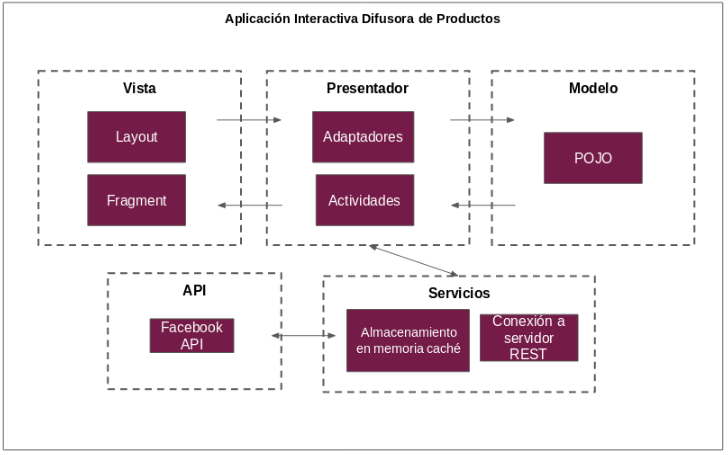
\includegraphics[width=.9 \textwidth]{imagenes/Arquitecturas/arquiCliente}
		\caption{Arquitectura del módulo AIDP.}
		\label{image:arquitecturaAIDP}
\end{figure}
\FloatBarrier

En la imagen mostrada anteriormente (Figura \ref{image:arquitecturaAIDP}) se pueden observar las 3 áreas principales que componen a dicha arquitectura, mismas que corresponden a una arquitectura MVP.
\begin{itemize}
\item Vista: Corresponde a los archivos .xml los cuales corresponden a los layouts y fragmentos que desplegarán la información visual a los clientes y usuarios de la aplicación.
\item Presentador: Correspondiente a las interfaces de los adaptadores y actividades, los cuales se encargan de interconectar las clases simples JAVA con los layouts y así mismo, del envío y recepción de peticiones al servidor REST y a la memoria caché del celular.
\item Modelo: Corresponde a los POJO, mismos que se refieren a clases simples JAVA.
\item  Servicios: Son tanto la conexión al servidor REST como el almacenamiento en memoria caché del dispositivo móvil.
\item API: Dentro de esta sección se encuentra la API de Facebook, utilizadas para obtener los datos e información del usuario.
\end{itemize}
%--------------------------------------------------
\subsection{Prototipo 1: Diseño inicial de la aplicación}
\hypertarget{Prototipo1}{}
%--------------------------------------------------
\subsubsection{Análisis}
Se ha definido previamente la problemática a resolver, identificando los componentes principales que deberán ser integrados al sistema, \cite{Etapas} para ello, se utilizan ciertas herramientas tales como la definición de requerimientos funcionales, que ha sido presentada previamente en el capítulo de ``Bosquejo general de la aplicación'' con el título de \hyperlink{RFAIDP}{``Requerimientos Funcionales de Aplicación Interactiva Difusora de Productos''}. En la sección de análisis se planifica la integración de dichos requerimientos con el fin de saber cuales son las funciones que se requieren para que la aplicación móvil funcione adecuadamente. 
\\ \par 
La figura \ref{image:casosdeusoAIDPP1} presenta los casos de uso del módulo de Aplicación Interactiva Difusora de Productos. En ella se observan 8 casos de uso de los cuales se extienden y se incluyen otros casos de uso a su vez. También es importante destacar que hay una dependencia para el caso de uso 6\_7.1 ``Añadir productos a favoritos''.
\\ \par


%CASOS USO
\title{\textbf{Casos de uso de AIDP}\\ \par}

\FloatBarrier
\begin{figure}[htbp!]
		\centering
			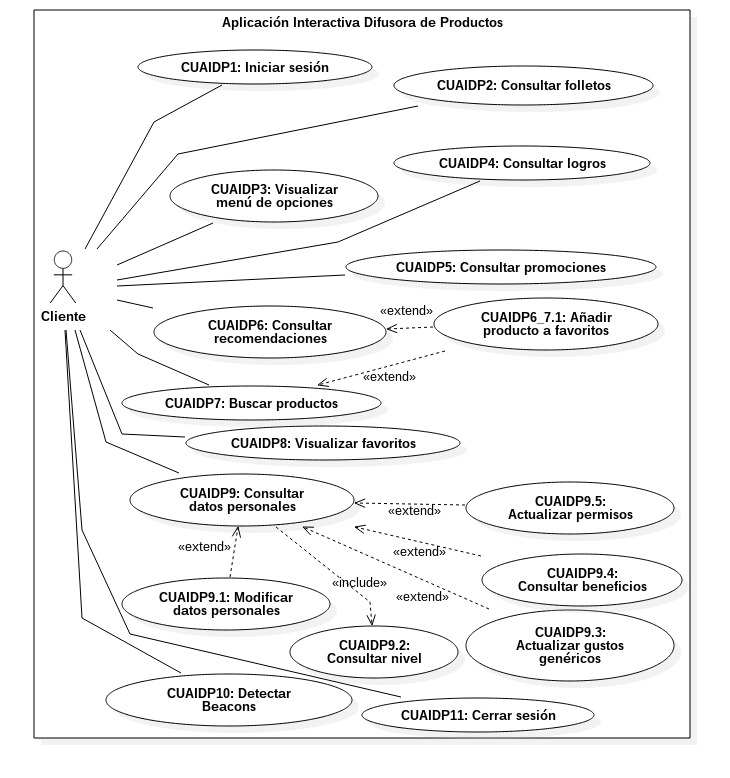
\includegraphics[width=.9 \textwidth]{imagenes/Diagramas_UserApp/casosDeUso_prototipo1}
		\caption{Casos de uso de la Aplicación Interactiva Difusora de Productos.}
		\label{image:casosdeusoAIDPP1}
\end{figure}
\FloatBarrier
\newpage
%--------------------------------------------------
\subsubsection{Diseño}
Posteriormente en esta etapa y a partir de los requerimientos definidos anteriormente, se muestran tanto el diagrama de casos de uso de la aplicación, como los diagramas de secuencia que permiten una mejor comprensión del funcionamiento que cada clase tendrá en el módulo. Así mismo, se muestra el flujo de navegación de la aplicación.
\\ \par
\title{\textbf{Diagrama de clases}\\ \par}
El diagrama de la figura \ref{image:clases} se dividió en 3 secciones para obtener una mejor visualización, dichas secciones corresponden a la figura \ref{image:clases1}, \ref{image:clases2} y \ref{image:clases3}.\\ \par 
\textit{Nota: Las clases mostradas en este prototipo muestran únicamente los métodos y atributos básicos de cada una de ellas debido a que estas no contemplan correctamente el funcionamiento que proveerá cada una de esas clases. Por dicha razón, en los prototipos posteriores se describirán  los elementos tanto de las clases que se han plasmado como de las que aún no han sido desarrolladas.}
\FloatBarrier
\begin{figure}[htbp!]
		\centering
			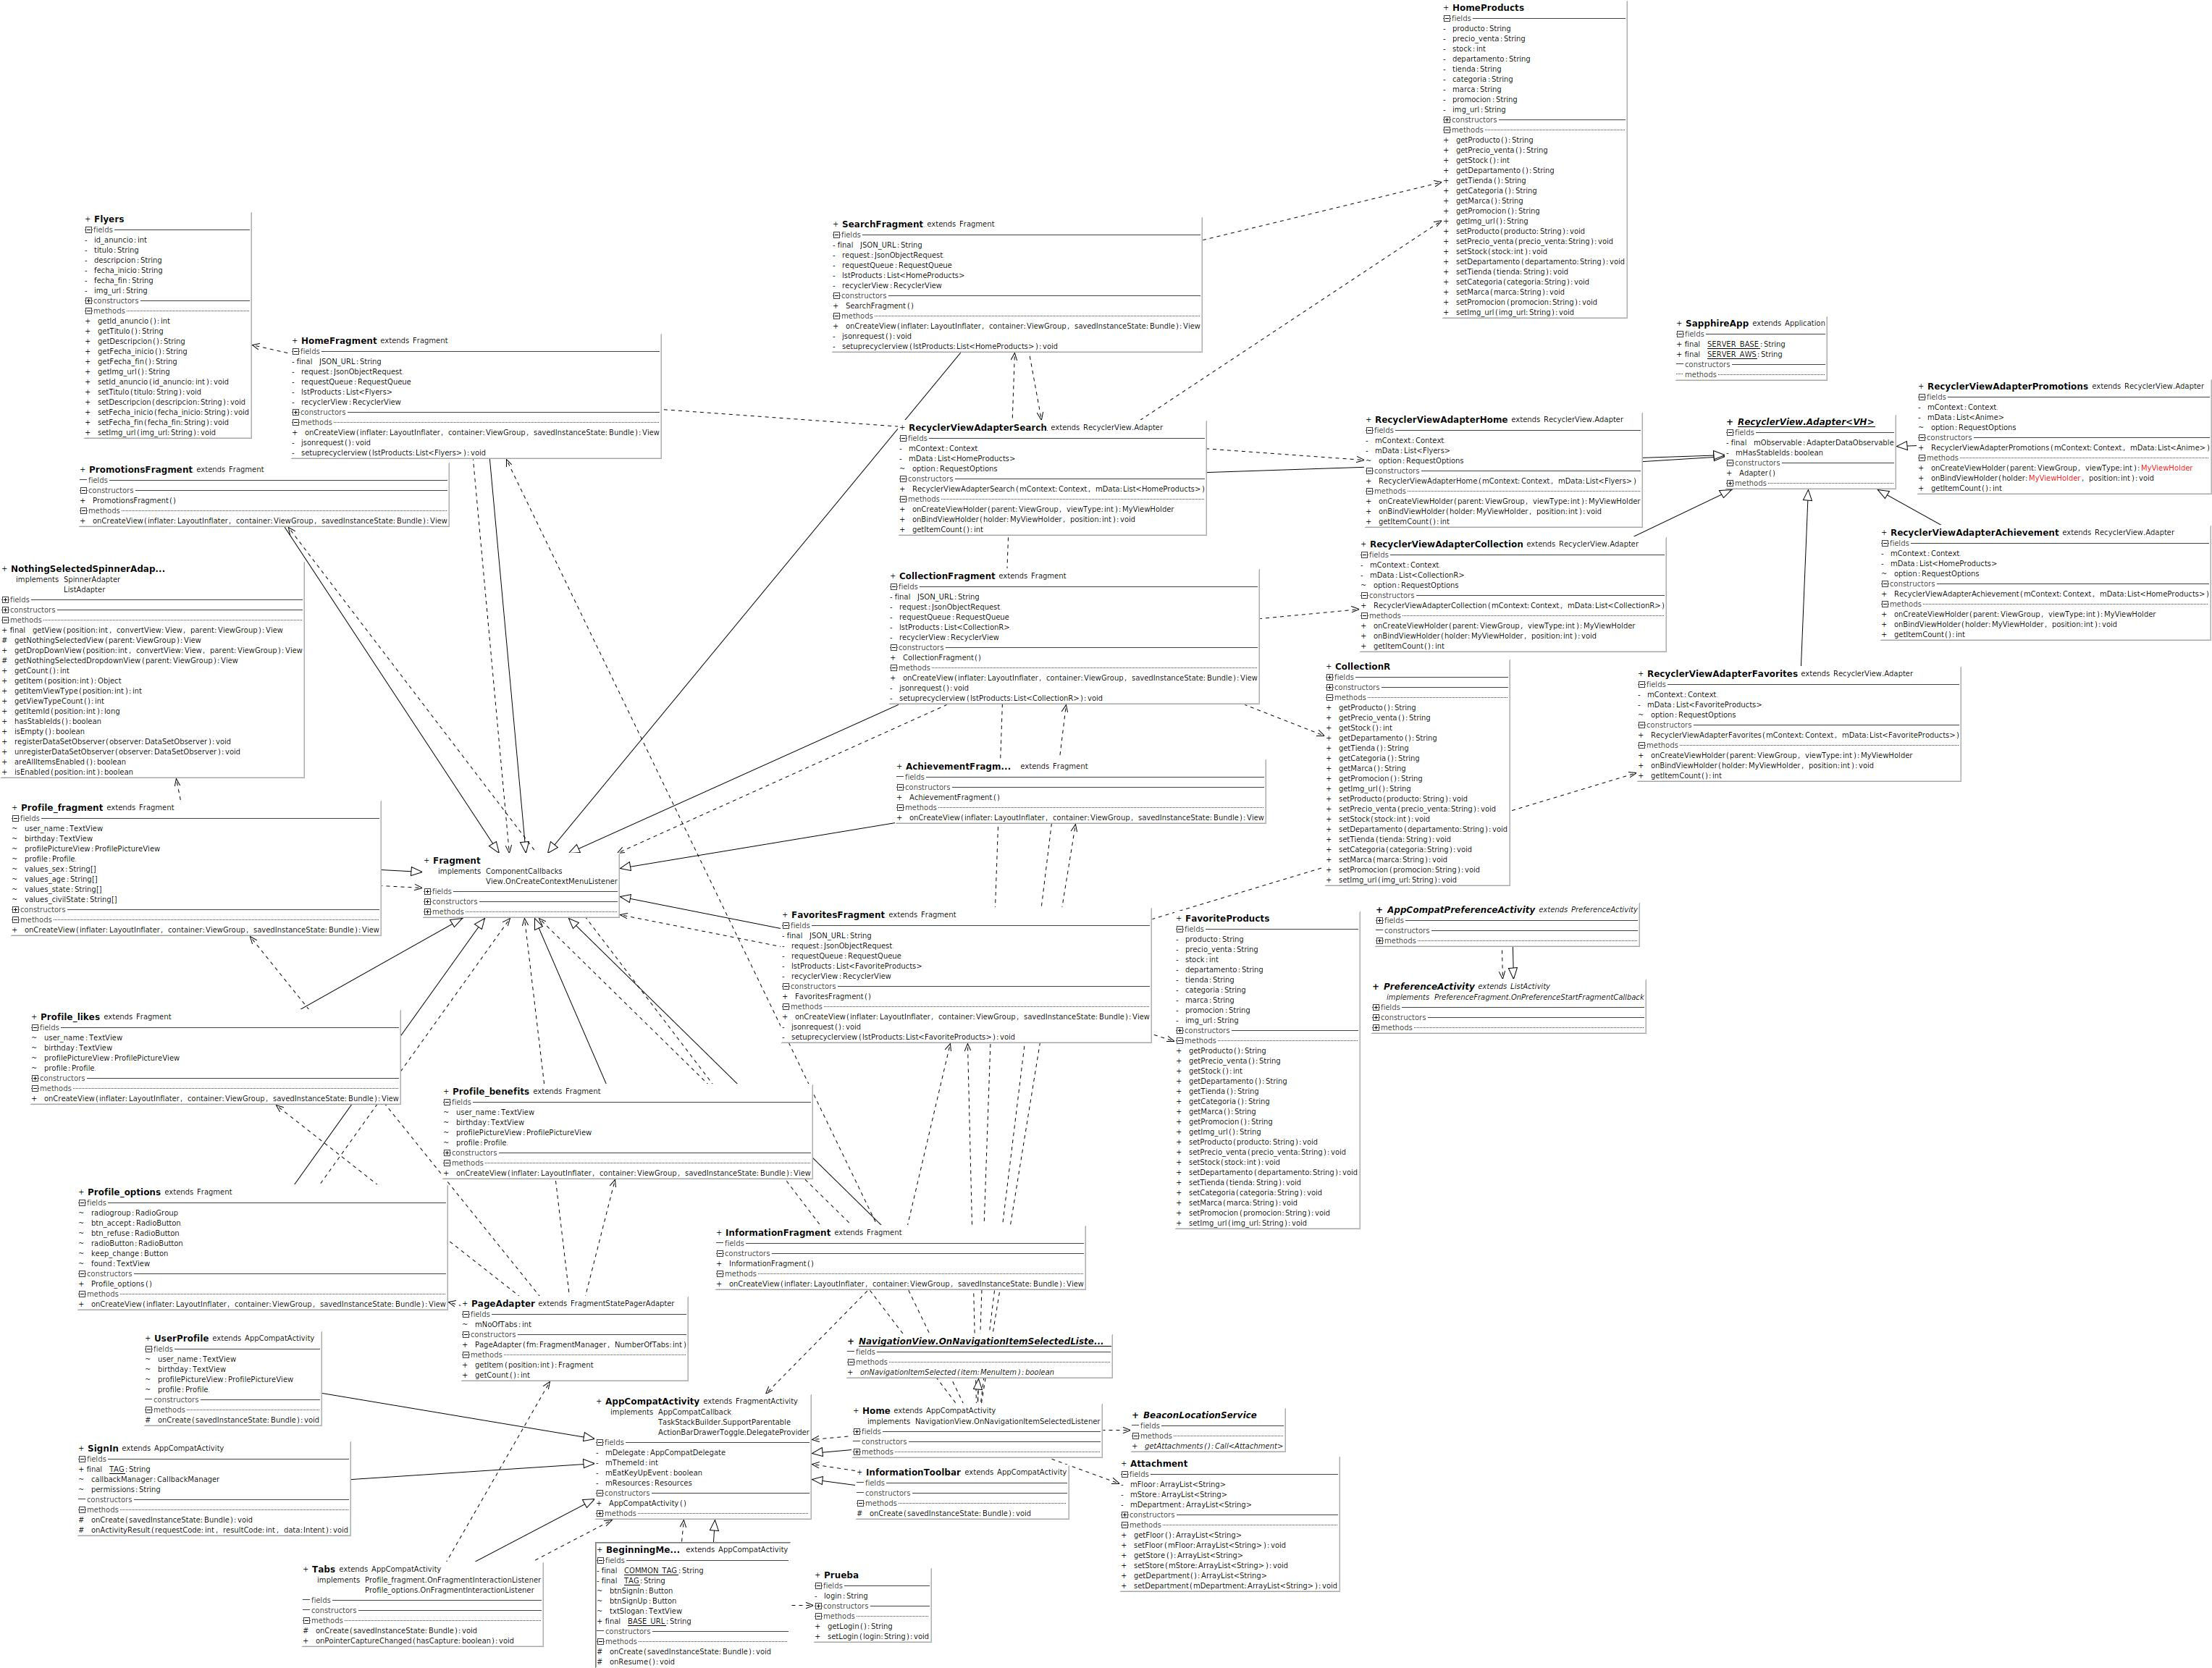
\includegraphics[width=1.1 \textwidth]{imagenes/Diagramas_UserApp/Nuevos_diagramas/diagrama2}
		\caption{Diagrama de clases (Visualización completa).}
		\label{image:clases}
\end{figure}
\FloatBarrier

\FloatBarrier
\begin{figure}[htbp!]
		\centering
			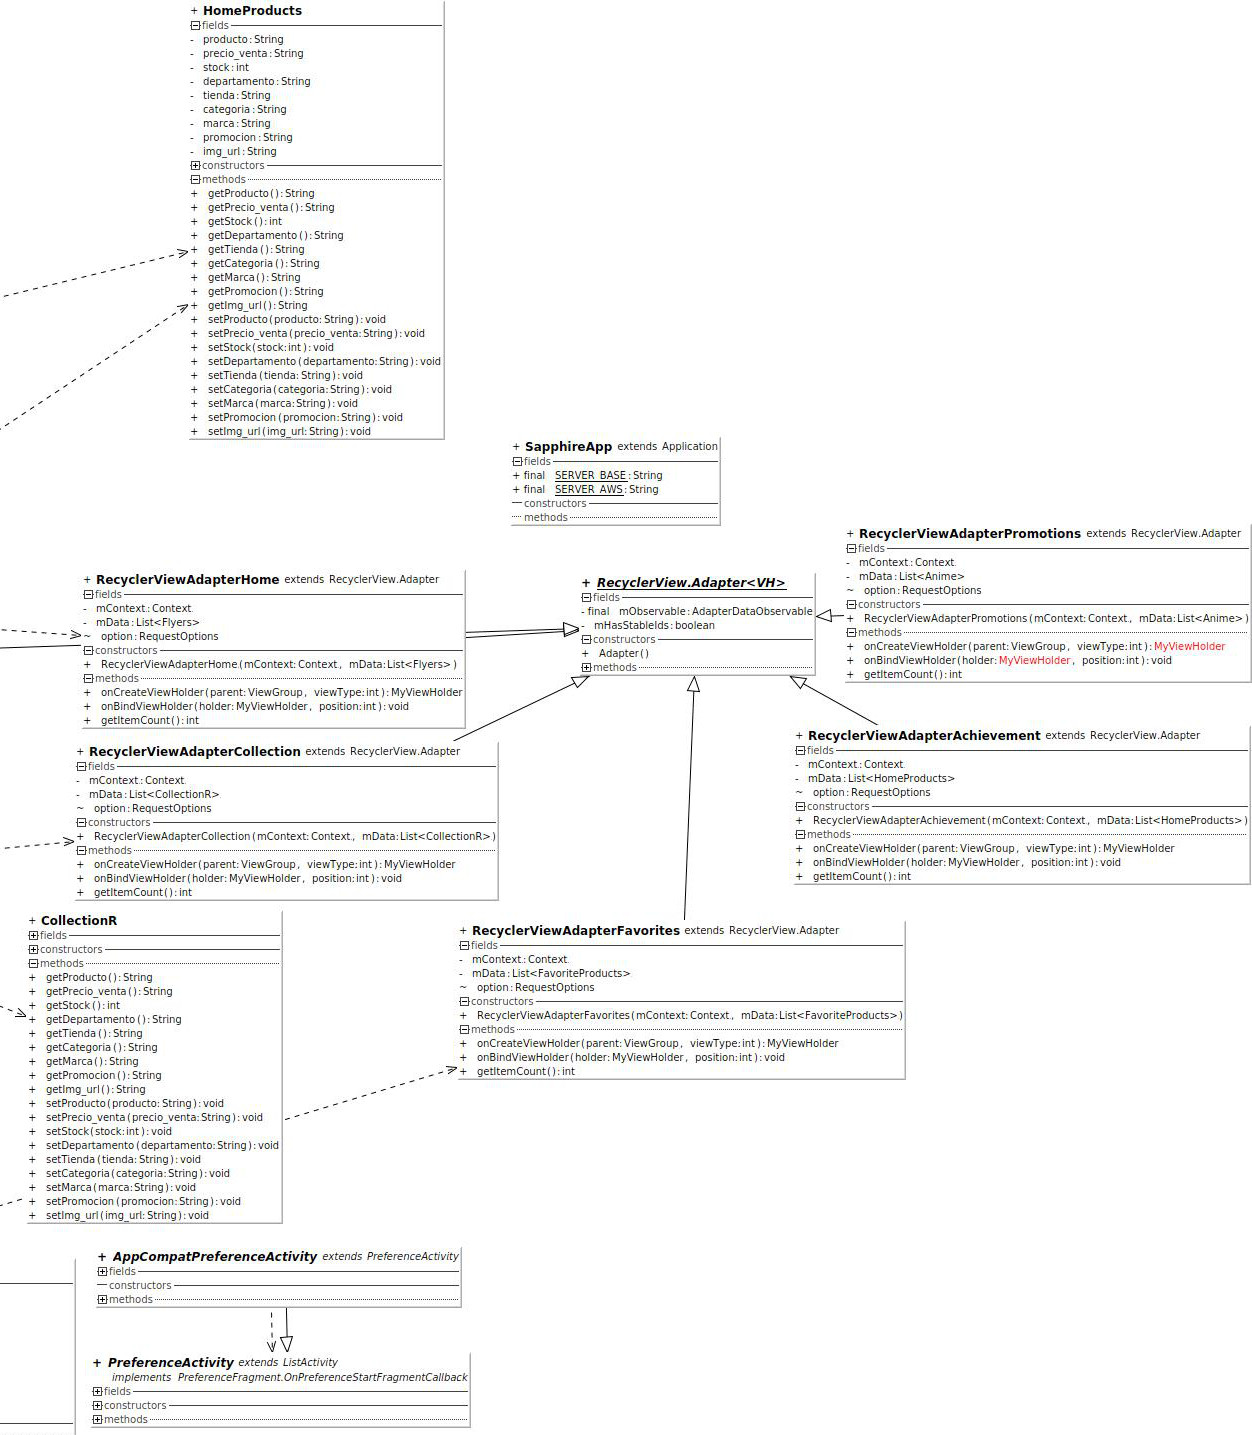
\includegraphics[width=1.1 \textwidth]{imagenes/Diagramas_UserApp/Nuevos_diagramas/diagrama2_1}
		\caption{Diagrama de clases (Parte 1).}
		\label{image:clases1}
\end{figure}
\FloatBarrier

\FloatBarrier
\begin{figure}[htbp!]
		\centering
			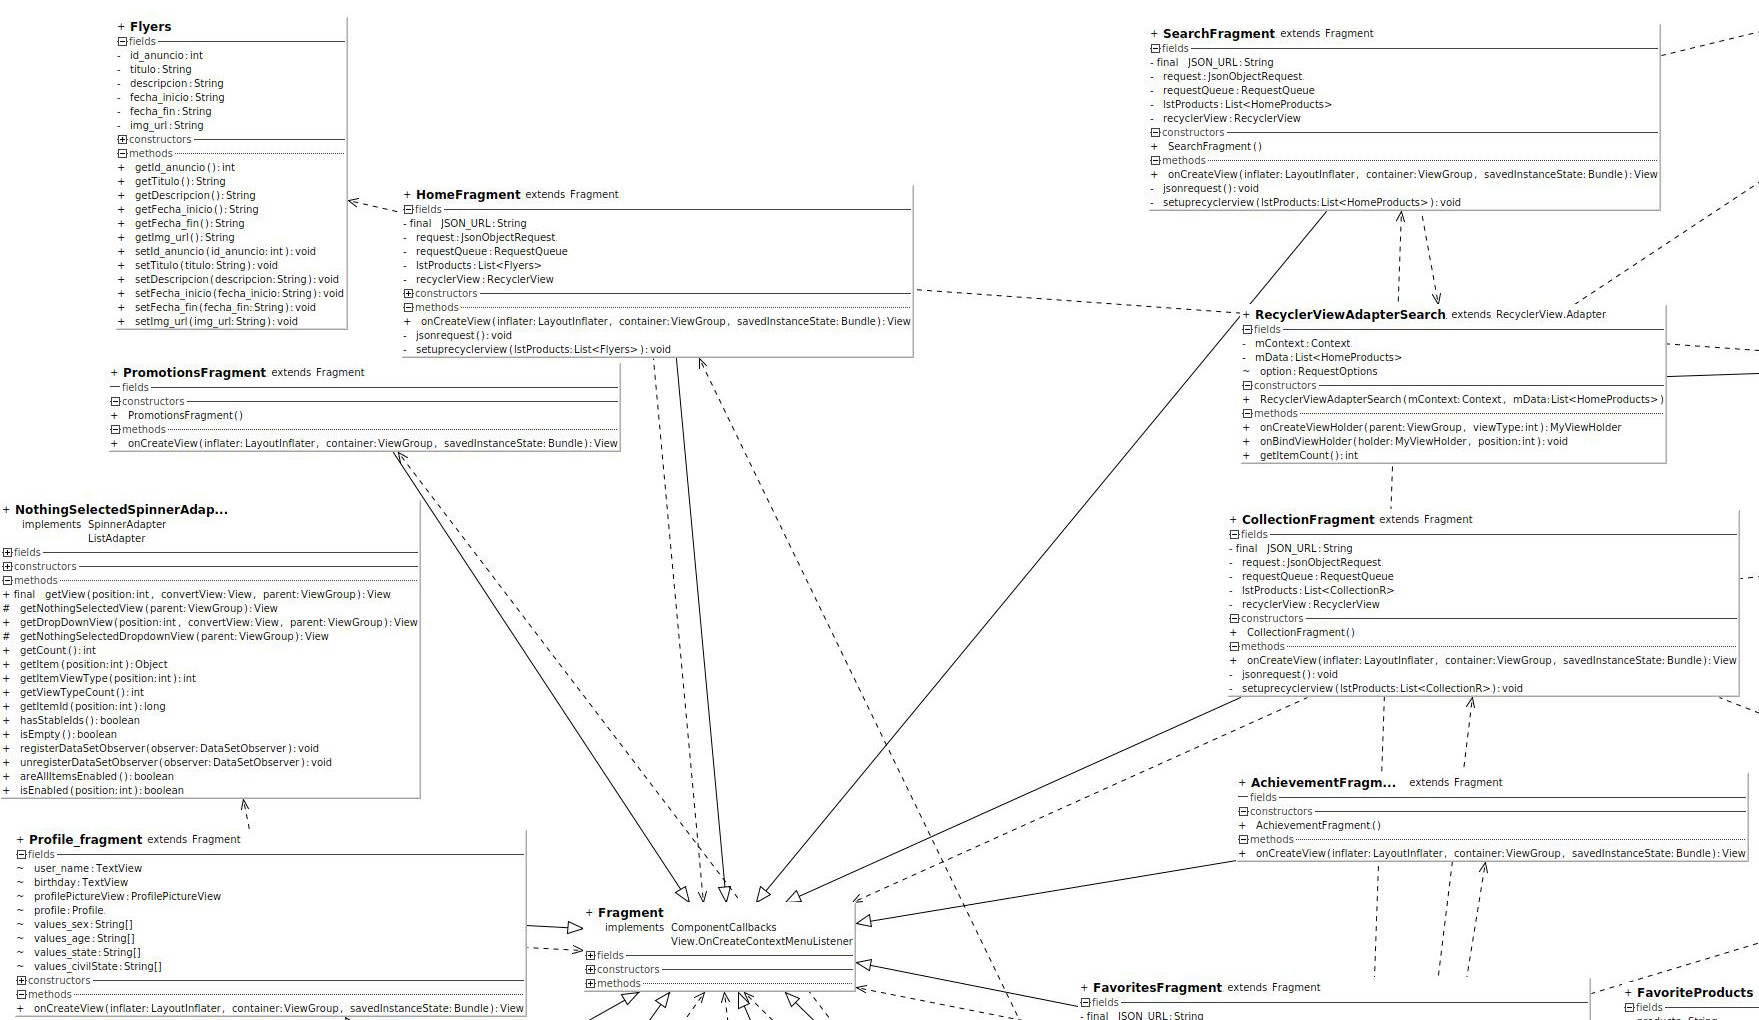
\includegraphics[width=1.1 \textwidth]{imagenes/Diagramas_UserApp/Nuevos_diagramas/diagrama2_2}
		\caption{Diagrama de clases (Parte 2).}
		\label{image:clases2}
\end{figure}
\FloatBarrier

\FloatBarrier
\begin{figure}[htbp!]
		\centering
			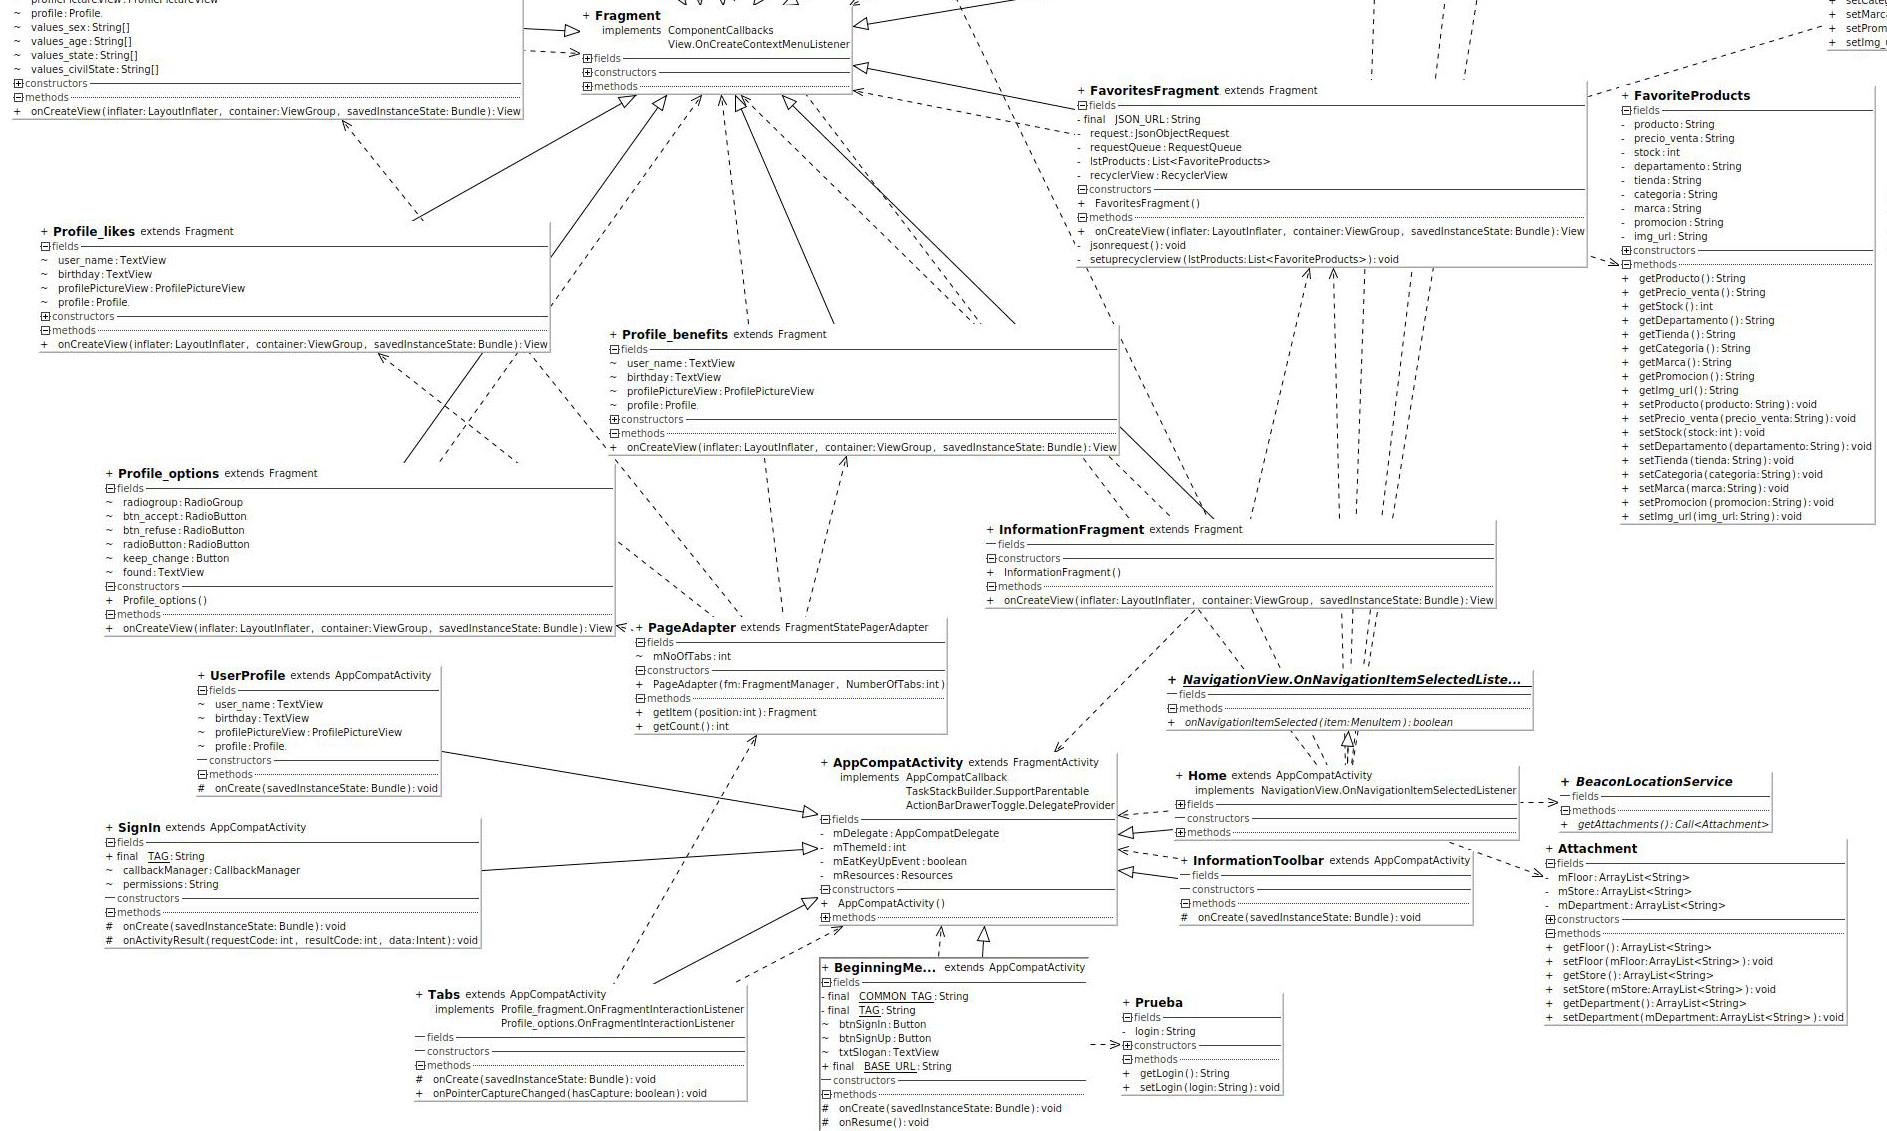
\includegraphics[width=1 \textwidth]{imagenes/Diagramas_UserApp/Nuevos_diagramas/diagrama2_3}
		\caption{Diagrama de clases (Parte 3).}
		\label{image:clases3}
\end{figure}
\FloatBarrier

\title{\textbf{Flujo de navegación de la Aplicación Interactiva Difusora de Productos}\\ \par}

En la figura \ref{Image:FlujoNavegacion1} se muestra el diagrama de como es el flujo de navegación de la aplicación del cliente, se ha divido en dos partes debido al tamaño de este, la figura \ref{Image:FlujoNavegacion2} y \ref{Image:FlujoNavegacion3}.
\FloatBarrier
\begin{figure}[htbp!]
		\centering
			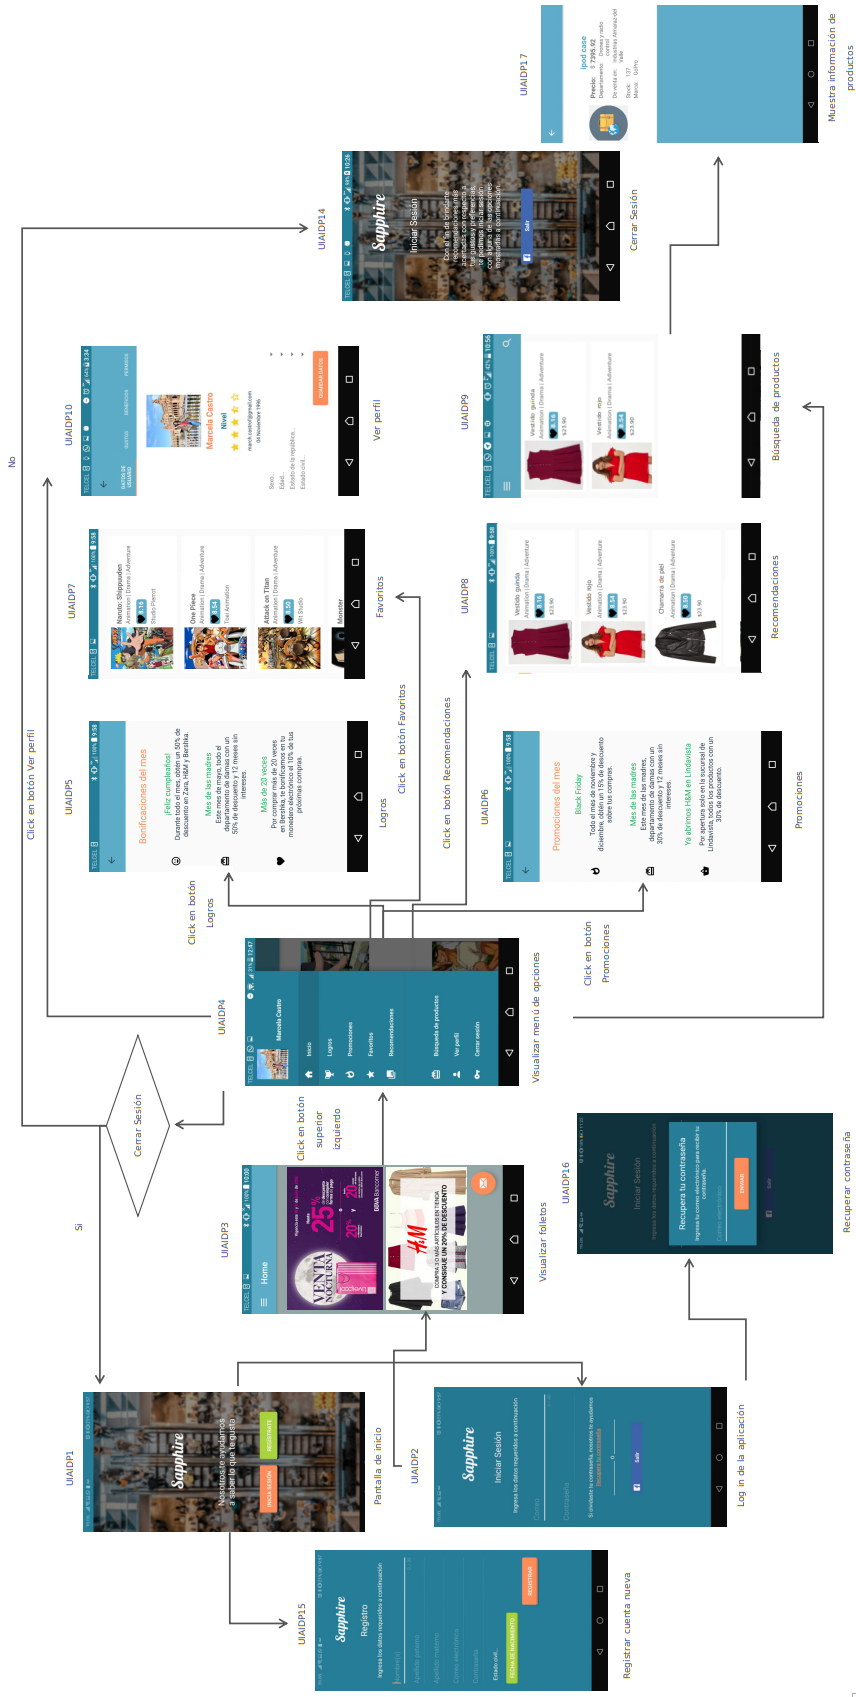
\includegraphics[width=.66 \textwidth]{imagenes/UI_userapp/mapaNav1H}
		\caption{Flujo de navegación de la Aplicación Interactiva Difusora de Productos (Visualización completa).}
		\label{Image:FlujoNavegacion1}
\end{figure}
\FloatBarrier

\FloatBarrier
\begin{figure}[htbp!]
		\centering
			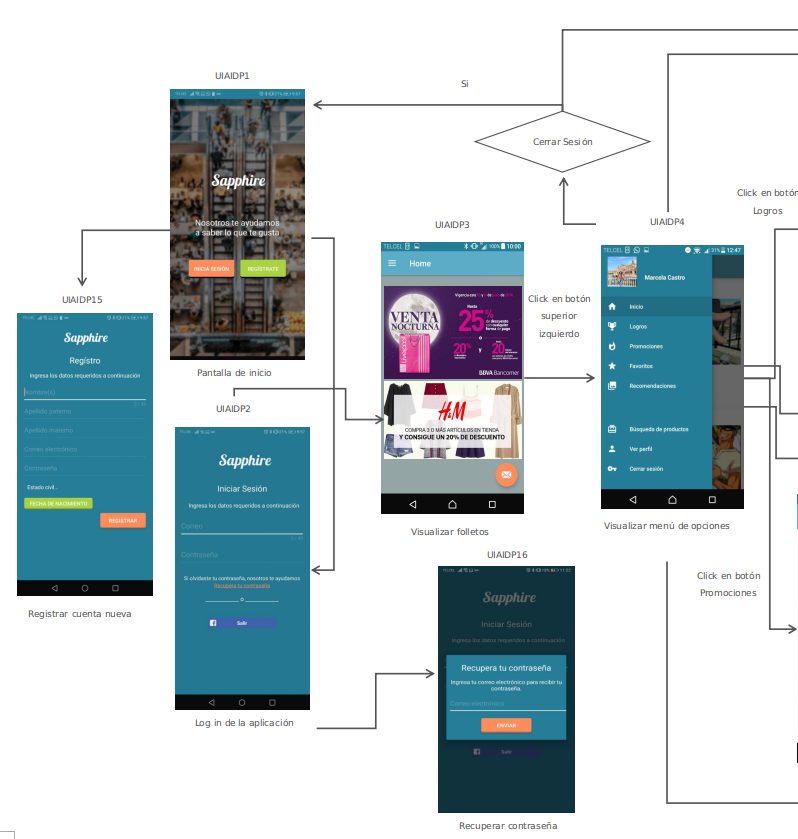
\includegraphics[width=1 \textwidth]{imagenes/UI_userapp/mapaNavP1}
		\caption{Flujo de navegación de la Aplicación Interactiva Difusora de Productos (Parte 1).}
		\label{Image:FlujoNavegacion2}
\end{figure}
\FloatBarrier

\FloatBarrier
\begin{figure}[htbp!]
		\centering
			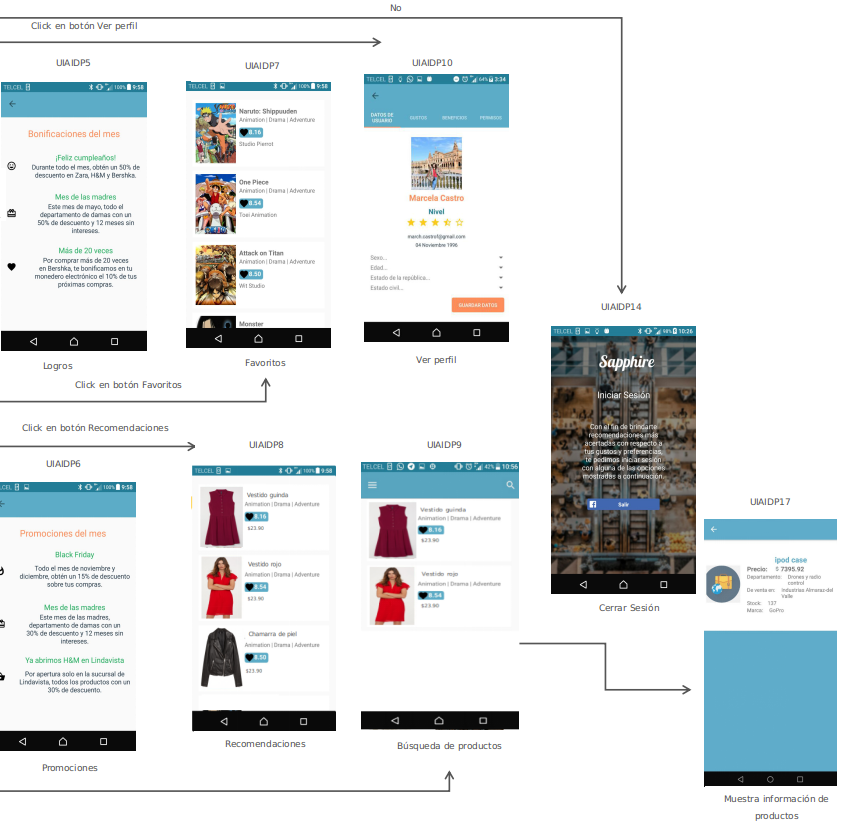
\includegraphics[width=1 \textwidth]{imagenes/UI_userapp/mapaNavP2}
		\caption{Flujo de navegación de la Aplicación Interactiva Difusora de Productos (Parte 2).}
		\label{Image:FlujoNavegacion3}
\end{figure}
\FloatBarrier

La figura \ref{image:flujoInicio} muestra 3 pantallas que son las vías alternativas para iniciar sesión por primera vez en la aplicación. El usuario puede elegir la opción de ingresar con su cuenta previa de Facebook, mediante el ingreso de otra cuenta diferente o por medio de la creación de una cuenta completamente nueva.
\FloatBarrier
\begin{figure}[htbp!]
		\centering
			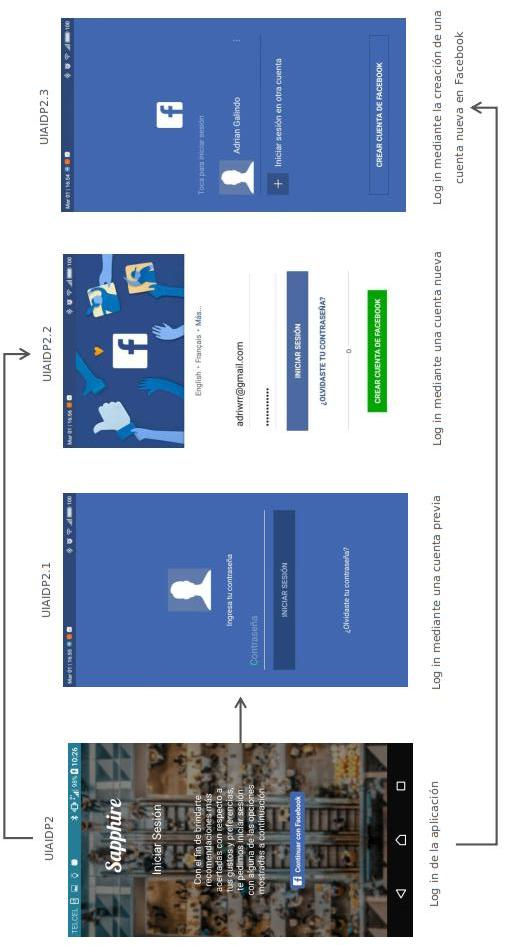
\includegraphics[width=.5 \textwidth]{imagenes/UI_userapp/mapaInicioH}
		\caption{Flujo de navegación de los métodos para iniciar sesión (Visualización completa).}
		\label{image:flujoInicio}		
\end{figure}
\FloatBarrier

La figura \ref{image:flujoNavegacionDifusoraDerivada1} muestra 4 pantallas que se derivan de una de las opciones del menú lateral principal ``Ver perfil'' mostrado en la figura \ref{Image:FlujoNavegacion1}, esta figura de igual manera fue divida en dos secciones (figura \ref{image:flujoNavegacionDifusoraDerivada2} y figura \ref{image:flujoNavegacionDifusoraDerivada3}) para una mejor visualización de su contenido.
\FloatBarrier
\begin{figure}[htbp!]
		\centering
			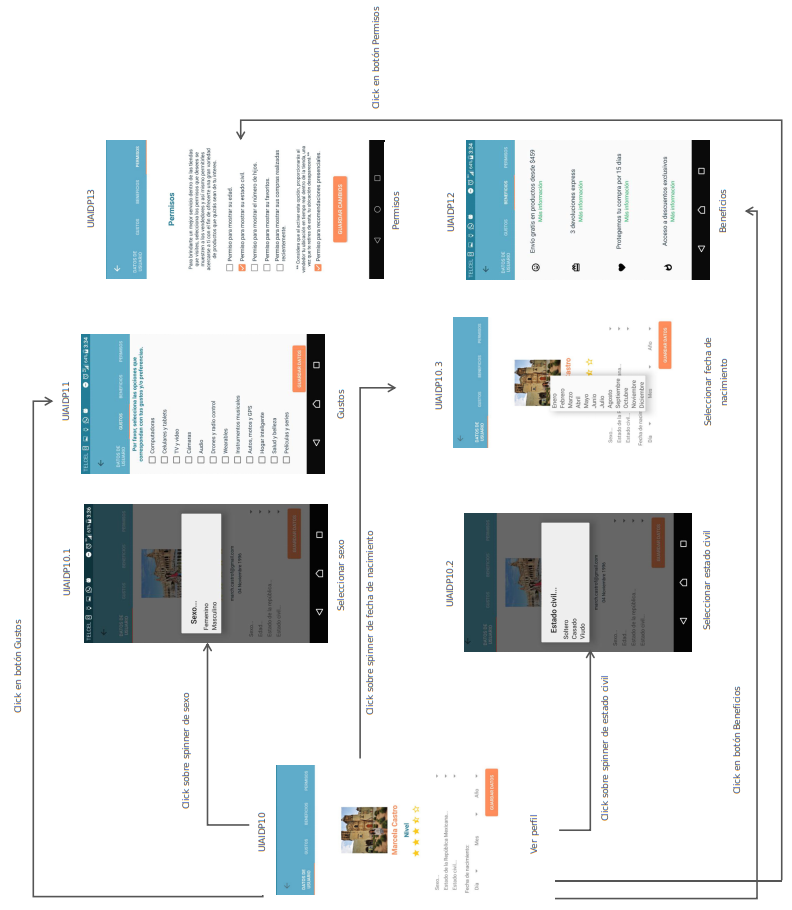
\includegraphics[width=1 \textwidth]{imagenes/UI_userapp/mapaNav2H}
		\caption{Flujo de navegación de la Aplicación Interactiva Difusora de Productos (Visualización completa).}
		\label{image:flujoNavegacionDifusoraDerivada1}		
\end{figure}
\FloatBarrier

\FloatBarrier
\begin{figure}[htbp!]
		\centering
			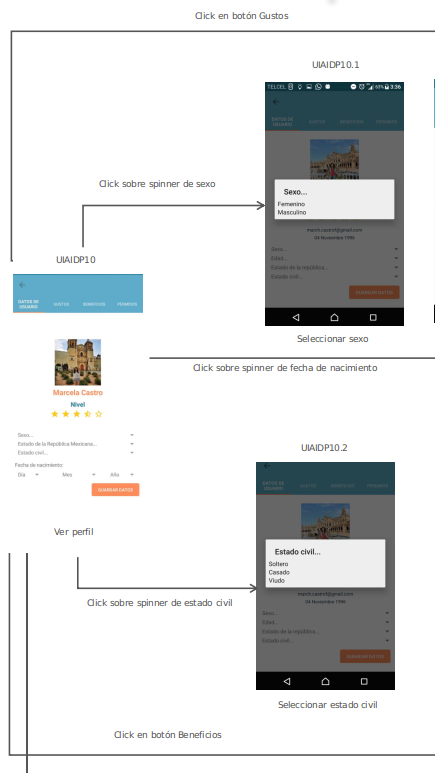
\includegraphics[width=.7 \textwidth]{imagenes/UI_userapp/mapNav2P1}
		\caption{Flujo de navegación de la Aplicación Interactiva Difusora de Productos (Parte 1).}
		\label{image:flujoNavegacionDifusoraDerivada2}
\end{figure}
\FloatBarrier

\FloatBarrier
\begin{figure}[htbp!]
		\centering
			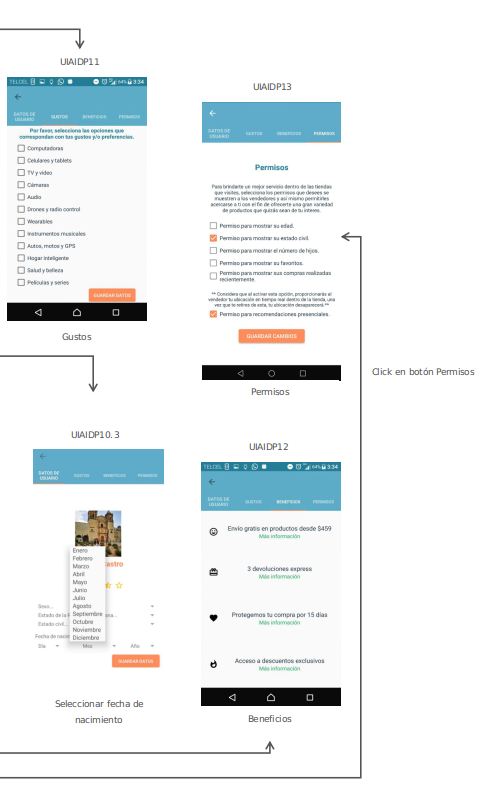
\includegraphics[width=.75 \textwidth]{imagenes/UI_userapp/mapaNav2P2}
		\caption{Flujo de navegación de la Aplicación Interactiva Difusora de Productos (Parte 2).}
		\label{image:flujoNavegacionDifusoraDerivada3}
\end{figure}
\FloatBarrier

%NAVEGACION PANTALLAS
\hypertarget{Pantallas}{}
\subparagraph{UIAIDP1 - Pantalla de inicio} ~\\
\FloatBarrier
\IUDescripcion
[.35] % Width
{UI_userapp/Begin} % Imagen sin la ruta 'imagen/'
{UIAIDP1} % Identificador
{Pantalla de inicio.}  % Etiqueta/nombre de la imagen
{Mostrar la pantalla inicial de la aplicación.} %Objetivo
{Esta pantalla (figura \ref{UIAIDP1}), aparece al iniciar la aplicación. Muestra el logo y slogan del proyecto y de igual manera proporciona la opción para iniciar sesión.} %Intro/Breve descripción de la pantalla
{Ninguna.} %Salidas
{Ninguna.} %Entradas
\FloatBarrier

\subparagraph{UIAIDP2 - Log in de la aplicación} ~\\
\FloatBarrier
\IUDescripcion
[.35] % Width
{UI_userapp/SignIn} % Imagen sin la ruta 'imagen/'
{UIAIDP2} % Identificador
{Log in de la aplicación.}  % Etiqueta/nombre de la imagen
{Mostrar las opciones de inicio de sesión.} %Objetivo
{La figura \ref{UIAIDP2}, es la pantalla que se muestra al usuario con el fin de informarles la opción que estos tienen para iniciar sesión e ingresar al sistema.} %Intro/Breve descripgción de la pantalla
{Ninguna.} %Salidas
{Correo electrónico y contraseña del usuario.} %Entradas
\FloatBarrier

\subparagraph{UIAIDP2.1 - Log in mediante una cuenta previa} ~\\
\FloatBarrier
\IUDescripcion
[.4] % Width
{UI_userapp/2} % Imagen sin la ruta 'imagen/'
{UIAIDP2.1} % Identificador
{Log in mediante una cuenta previa.}  % Etiqueta/nombre de la imagen
{Mostrar una opción para el inicio de sesión.} %Objetivo
{La figura \ref{UIAIDP2.1}, es la pantalla que se muestra al usuario para que este ingrese su contraseña y agilizar de esta forma el inicio de sesión a la aplicación.} %Intro/Breve descripgción de la pantalla
{Ninguna.} %Salidas
{Contraseña del usuario.} %Entradas
\FloatBarrier

\subparagraph{UIAIDP2.2 - Log in mediante una cuenta nueva} ~\\
\FloatBarrier
\IUDescripcion
[.4] % Width
{UI_userapp/1} % Imagen sin la ruta 'imagen/'
{UIAIDP2.2} % Identificador
{Log in mediante una cuenta nueva.}  % Etiqueta/nombre de la imagen
{Mostrar una opción para el inicio de sesión.} %Objetivo
{La figura \ref{UIAIDP2.2}, es la pantalla que se muestra al usuario para que este ingrese una cuenta diferente a la que ya tenga registrada en la aplicación móvil.} %Intro/Breve descripgción de la pantalla
{Ninguna.} %Salidas
{Correo electrónico y contraseña del usuario.} %Entradas
\FloatBarrier

\subparagraph{UIAIDP2.3 - Log in mediante la creación de una cuenta nueva en Facebook} ~\\
\FloatBarrier
\IUDescripcion
[.4] % Width
{UI_userapp/3} % Imagen sin la ruta 'imagen/'
{UIAIDP2.3} % Identificador
{Log in mediante la creación de una cuenta nueva en Facebook.}  % Etiqueta/nombre de la imagen
{Mostrar las opciones de inicio de sesión.} %Objetivo
{La figura \ref{UIAIDP2.3}, es la pantalla que se muestra al usuario en la cual puede seleccionar la opción de creación de una cuenta completamente nueva.} %Intro/Breve descripgción de la pantalla
{Ninguna.} %Salidas
{Correo electrónico, contraseña y nombre de perfil.} %Entradas
\FloatBarrier

\subparagraph{UIAIDP2.4 - Log in solicitado por la API de Facebook} ~\\
\FloatBarrier
\IUDescripcion
[.35] % Width
{UI_userapp/4} % Imagen sin la ruta 'imagen/'
{UIAIDP2.4} % Identificador
{Log in solicitado por la API de Facebook.}  % Etiqueta/nombre de la imagen
{Realizar el inicio de sesión en la aplicación Sapphire utilizando la API de Facebook.} %Objetivo
{La figura \ref{UIAIDP2.4}, muestra la pantalla en la cual el usuario deberá ingresar su correo electrónico y contraseña de Facebook con el fin de iniciar sesión en la aplicación de Sapphire por medio de su cuenta de Facebook.} %Intro/Breve descripgción de la pantalla
{Ninguna.} %Salidas
{Correo electrónico y contraseña.} %Entradas
\FloatBarrier

\subparagraph{UIAIDP3 - Visualizar folletos} ~\\
\FloatBarrier
\IUDescripcion
[.4] % Width
{UI_userapp/Home} % Imagen sin la ruta 'imagen/'
{UIAIDP3} % Identificador
{Visualizar folletos.}  % Etiqueta/nombre de la imagen
{Mostrar las promociones y productos con descuento.} %Objetivo
{La figura \ref{UIAIDP3}, muestra la pantalla de los diferentes productos que se encuentran en las diferentes tiendas y que cuentan con algún descuento o promoción en particular. Cumple la función de un folleto o propaganda proporcionado al ingresar a una tienda.} %Intro/Breve descripción de la pantalla
{Ninguna.} %Salidas
{Ninguna.} %Entradas
\FloatBarrier

\subparagraph{UIAIDP3.1 - Detectar Beacons} ~\\
\FloatBarrier
\IUDescripcion
[.4] % Width
{UI_userapp/beacon} % Imagen sin la ruta 'imagen/'
{UIAIDP3.1} % Identificador
{Detectar Beacons.}  % Etiqueta/nombre de la imagen
{Mostrar alerta al usuario al detectar un Beacon.} %Objetivo
{La figura \ref{UIAIDP3.1}, muestra la pantalla anterior ``UIAIDP3 - Visualizar folletos'' en la cual se despliega una pequeña alerta en la parte inferior con la cuál se le notifica al cliente que ha ingresado a un nuevo piso o departamento.} %Intro/Breve descripción de la pantalla
{Ninguna.} %Salidas
{Ninguna.} %Entradas
\FloatBarrier

\subparagraph{UIAIDP4 - Visualizar menú de opciones} ~\\
\FloatBarrier
\IUDescripcion
[.4] % Width
{UI_userapp/Menu2} % Imagen sin la ruta 'imagen/'
{UIAIDP4} % Identificador
{Visualizar menú de opciones.}  % Etiqueta/nombre de la imagen
{Mostrar las opciones de navegación con las que el usuario cuenta.} %Objetivo
{La pantalla inferior (figura \ref{UIAIDP4}),  muestra un menú en la parte superior izquierda el cual despliega las diferentes opciones en las que el usuario puede encontrar ofertas o productos de su agrado.} %Intro/Breve descripción de la pantalla
{Ninguna.} %Salidas
{Ninguna.} %Entradas
\FloatBarrier

\subparagraph{UIAIDP5 - Logros} ~\\
\FloatBarrier
\IUDescripcion
[.4] % Width
{UI_userapp/Bonificaciones} % Imagen sin la ruta 'imagen/'
{UIAIDP5} % Identificador
{Logros.}  % Etiqueta/nombre de la imagen
{Mostrar las bonificaciones que las tiendas tienen con motivo de una fecha especial.} %Objetivo
{En la figura \ref{UIAIDP5}, el usuario visualiza las bonificaciones que se realizan al usuario con motivo de una fecha especial en el mes como su cumpleaños o navidad, por ejemplo.} %Intro/Breve descripción de la pantalla
{Ninguna.} %Salidas
{Ninguna.} %Entradas
\FloatBarrier

\subparagraph{UIAIDP6 - Promociones} ~\\
\FloatBarrier
\IUDescripcion
[.4] % Width
{UI_userapp/Promociones} % Imagen sin la ruta 'imagen/'
{UIAIDP6} % Identificador
{Promociones.}  % Etiqueta/nombre de la imagen
{Mostrar las promociones que las tiendas ofrecen al cliente.} %Objetivo
{Las diferentes promociones que se realizan en un mes en específico por ejemplo en diciembre, el ``Black Friday'' o descuentos por el día de las madres, son mostradas en esta pantalla (figura \ref{UIAIDP6}).} %Intro/Breve descripción de la pantalla
{Ninguna.} %Salidas
{Ninguna.} %Entradas
\FloatBarrier

\subparagraph{UIAIDP7 - Favoritos} ~\\
\FloatBarrier
\IUDescripcion
[.4] % Width
{UI_userapp/Favoritos} % Imagen sin la ruta 'imagen/'
{UIAIDP7} % Identificador
{Favoritos.}  % Etiqueta/nombre de la imagen
{Mostrar los productos que el cliente ha marcado como favoritos.} %Objetivo
{La figura \ref{UIAIDP7} muestra la  pantalla en la que el cliente puede visualizar los productos que previamente ha marcado como favoritos.} %Intro/Breve descripción de la pantalla
{Ninguna.} %Salidas
{Ninguna.} %Entradas
\FloatBarrier

\subparagraph{UIAIDP8 - Recomendaciones} ~\\
\FloatBarrier
\IUDescripcion
[.4] % Width
{UI_userapp/Recomendaciones} % Imagen sin la ruta 'imagen/'
{UIAIDP8} % Identificador
{Recomendaciones.}  % Etiqueta/nombre de la imagen
{Mostrar las recomendaciones generadas por el módulo de recomendaciones FC.} %Objetivo
{La imagen de la figura \ref{UIAIDP8} presenta la pantalla donde se muestran todos los productos que han sido recomendados por parte del módulo de recomendaciones, mismos que han sido seleccionados con base a los gustos del cliente.} %Intro/Breve descripción de la pantalla
{Ninguna.} %Salidas
{Ninguna.} %Entradas
\FloatBarrier

\subparagraph{UIAIDP9 - Búsqueda de productos} ~\\
\FloatBarrier
\IUDescripcion
[.4] % Width
{UI_userapp/Busqueda} % Imagen sin la ruta 'imagen/'
{UIAIDP9} % Identificador
{Búsqueda de productos.}  % Etiqueta/nombre de la imagen
{Desplegar los productos que busque el cliente.} %Objetivo
{En la figura \ref{UIAIDP9} que muestra la pantalla  de búsqueda de productos, el usuario tiene la opción de buscar los productos que sean de su interés por ejemplo un vestido y visualizarlos según sean localizados.} %Intro/Breve descripción de la pantalla
{Ninguna.} %Salidas
{Ninguna.} %Entradas
\FloatBarrier

\subparagraph{UIAIDP10 - Ver perfil} ~\\
\FloatBarrier
\IUDescripcion
[.35] % Width
{UI_userapp/Perfil1} % Imagen sin la ruta 'imagen/'
{UIAIDP10} % Identificador
{Ver perfil.}  % Etiqueta/nombre de la imagen
{Visualizar los datos del usuario.} %Objetivo
{Esta pantalla (figura \ref{UIAIDP10}), despliega los datos y la imagen del usuario y de igual manera, proporciona al usuario la posibilidad de modificar ciertos datos específicos tales como su edad y estado civil.} %Intro/Breve descripción de la pantalla
{Ninguna.} %Salidas
{Sexo, edad y estado civil.} %Entradas
\FloatBarrier

\subparagraph{UIAIDP10.1 - Seleccionar sexo} ~\\
\FloatBarrier
\IUDescripcion
[.4] % Width
{UI_userapp/sexo} % Imagen sin la ruta 'imagen/'
{UIAIDP10.1} % Identificador
{Seleccionar sexo.}  % Etiqueta/nombre de la imagen
{Seleccionar el sexo del usuario.} %Objetivo
{La figura \ref{UIAIDP10.1} se muestra el despliegue de las dos diferentes opciones para que el usuario elija el sexo que corresponde.} %Intro/Breve descripción de la pantalla
{Ninguna.} %Salidas
{Sexo.} %Entradas
\FloatBarrier

\subparagraph{UIAIDP10.2 - Seleccionar estado civil} ~\\
\FloatBarrier
\IUDescripcion
[.4] % Width
{UI_userapp/edoCivil} % Imagen sin la ruta 'imagen/'
{UIAIDP10.4} % Identificador
{Seleccionar estado civil.}  % Etiqueta/nombre de la imagen
{Seleccionar su estado civil actual.} %Objetivo
{La figura \ref{UIAIDP10.4} se muestra el despliegue de los estados civiles de los que el usuario seleccionará su opción.} %Intro/Breve descripción de la pantalla
{Ninguna.} %Salidas
{Estado civil.} %Entradas
\FloatBarrier


\subparagraph{UIAIDP10.3 - Seleccionar fecha de nacimiento} ~\\
\FloatBarrier
\IUDescripcion
[.35] % Width
{UI_userapp/edad} % Imagen sin la ruta 'imagen/'
{UIAIDP10.2} % Identificador
{Seleccionar fecha de nacimiento.}  % Etiqueta/nombre de la imagen
{Seleccionar la fecha de nacimiento del usuario.} %Objetivo
{La figura \ref{UIAIDP10.2} se muestra el despliegue de los 3 datos que conforman la fecha de nacimiento.} %Intro/Breve descripción de la pantalla
{Ninguna.} %Salidas
{Día, mes y año de nacimiento.} %Entradas
\FloatBarrier

\subparagraph{UIAIDP11 - Gustos} ~\\
\FloatBarrier
\IUDescripcion
[.4] % Width
{UI_userapp/gustos} % Imagen sin la ruta 'imagen/'
{UIAIDP11} % Identificador
{Gustos.}  % Etiqueta/nombre de la imagen
{Elegir los gustos que se asemejen más a los del usuario.} %Objetivo
{Esta pantalla (figura \ref{UIAIDP11}), muestra una serie de categorías diferentes que el usuario puede o no seleccionar según correspondan con sus gustos.} %Intro/Breve descripción de la pantalla
{Ninguna.} %Salidas
{Gustos.} %Entradas
\FloatBarrier

\subparagraph{UIAIDP12 - Beneficios} ~\\
\FloatBarrier
\IUDescripcion
[.4] % Width
{UI_userapp/beneficios} % Imagen sin la ruta 'imagen/'
{UIAIDP12} % Identificador
{Beneficios.}  % Etiqueta/nombre de la imagen
{Consultar los beneficios que ofrece el nivel.} %Objetivo
{La figura \ref{UIAIDP12} muestra la sección de Beneficios en la que dependiendo el nivel en el que se encuentre el cliente, este obtendrá diferentes beneficios que serán más atractivos para el usuario entre más alto sea su nivel.} %Intro/Breve descripción de la pantalla
{Ninguna.} %Salidas
{Ninguna.} %Entradas
\FloatBarrier

\subparagraph{UIAIDP13 - Permisos} ~\\
\FloatBarrier
\IUDescripcion
[.33] % Width
{UI_userapp/permisos} % Imagen sin la ruta 'imagen/'
{UIAIDP13} % Identificador
{Proporcionar permisos.}  % Etiqueta/nombre de la imagen
{Solicitar al cliente permiso para mostrar en la aplicación de vendedor los diferentes permisos.} %Objetivo
{La figura \ref{UIAIDP13} muestra los permisos de los cuales el cliente decidirá si va a permitir a los vendedores tanto aproximarse a él para ofrecerle diferentes productos que pueden resultar de su interés, como visualizar su información básica personal.} %Intro/Breve descripción de la pantalla
{Ninguna.} %Salidas
{Permisos.} %Entradas
\FloatBarrier

\subparagraph{UIAIDP14 - Cerrar sesión} ~\\
\FloatBarrier
\IUDescripcion
[.4] % Width
{UI_userapp/SignOut} % Imagen sin la ruta 'imagen/'
{UIAIDP14} % Identificador
{Cerrar sesión.}  % Etiqueta/nombre de la imagen
{Cerrar la sesión activa.} %Objetivo
{Esta pantalla (figura \ref{UIAIDP14}), muestra una de las opciones que el usuario tiene para cerrar su sesión dentro de la aplicación, también puede hacer dicha acción desde el menú de opciones, presionando el último botón ``Cerrar sesión''.} %Intro/Breve descripción de la pantalla
{Ninguna.} %Salidas
{Ninguna.} %Entradas
\FloatBarrier

\subsection{Prototipo 2: Conexión de la AIDP con Beacon}
\subsubsection{Análisis}
Dentro de este prototipo se satisface el requerimiento funcional \hyperlink{RFAIDP}{Detectar Beacons}, definido previamente en el capítulo del ``Bosquejo general de la aplicación''  con el título de ``Requerimientos funcionales de la Aplicación Interactiva Difusora de Productos (RFAIDP)'' y mismo que ya ha sido contemplado en los casos de uso mostrados en la figura \ref{image:casosdeusoAIDP} en el prototipo 1. \\ \par
\subsubsection{Diseño}
En el prototipo siguiente, se añadió a la AIDP la conexión con los Beacon, se muestra a continuación el diagrama de secuencia que muestra el funcionamiento que realiza la aplicación al detectar dicho dispositivo cerca. \\ \par
\title{\textbf{Diagramas de secuencia}\\ \par}
\title{\textbf{Detectar Beacons}}
\\ \par
El diagrama de la figura \ref{image:detecta} muestra la secuencia desarrollada con el fin de obtener las zonas de proximidad de los Beacons y así poder mostrar en el dispositivo del cliente una alerta cuando este ingrese a dicha zona.
\FloatBarrier
\begin{figure}[htbp!]
		\centering
			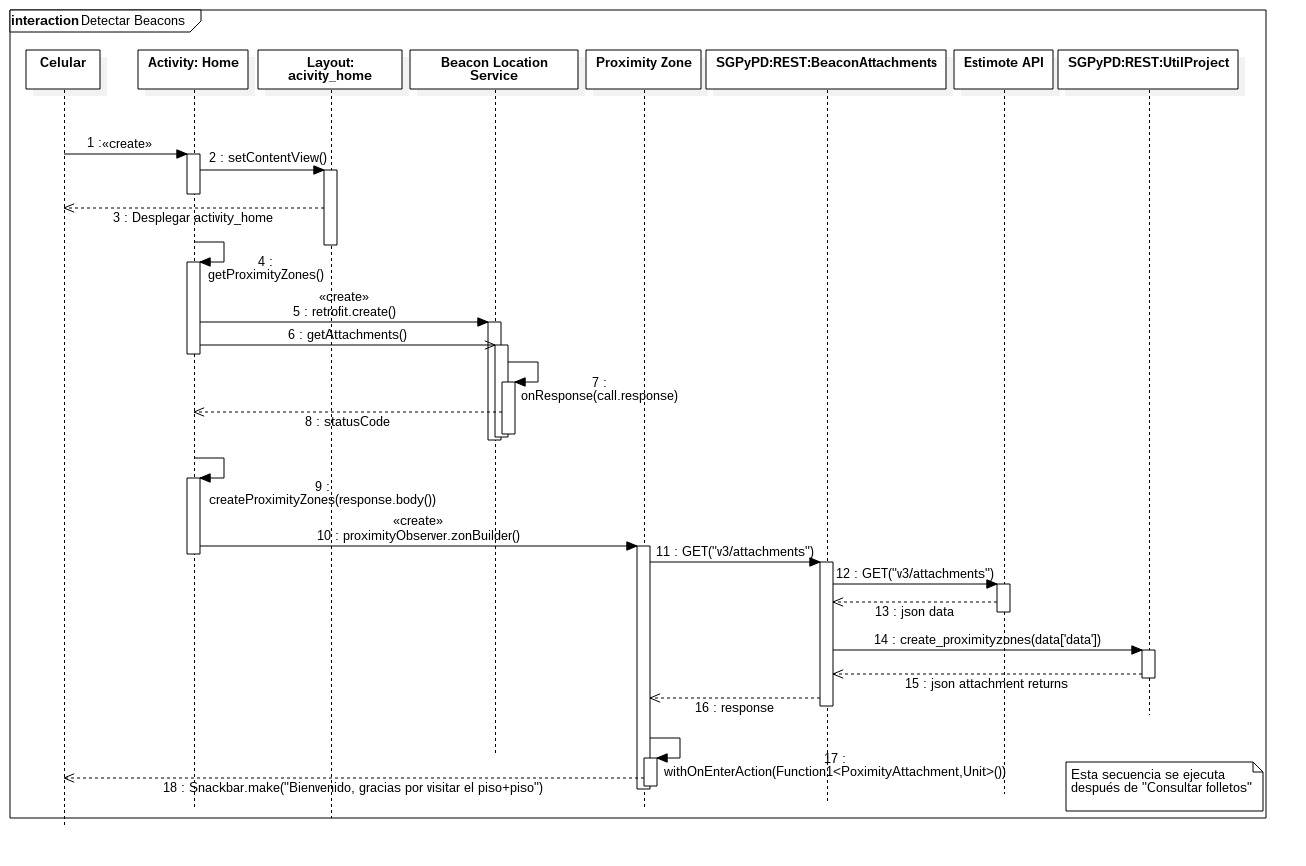
\includegraphics[width=1.1 \textwidth]{imagenes/Diagramas_UserApp/Nuevos_diagramas/detectarBeacons}
		\caption{Diagrama de secuencia para detectar Beacons (Visualización completa).}
		\label{image:detecta}
\end{figure}
\FloatBarrier


El diagrama de la figura \ref{image:detecta2} se dividió en dos secciones con el fin de mostrar una mejor visualización. Dicho diagrama muestra la secuencia desarrollada con el fin de obtener las zonas de proximidad de los Beacons, sin embargo a este se le añade también la funcionalidad de publicar la ubicación del cliente en Kafka.
\FloatBarrier
\begin{figure}[htbp!]
		\centering
			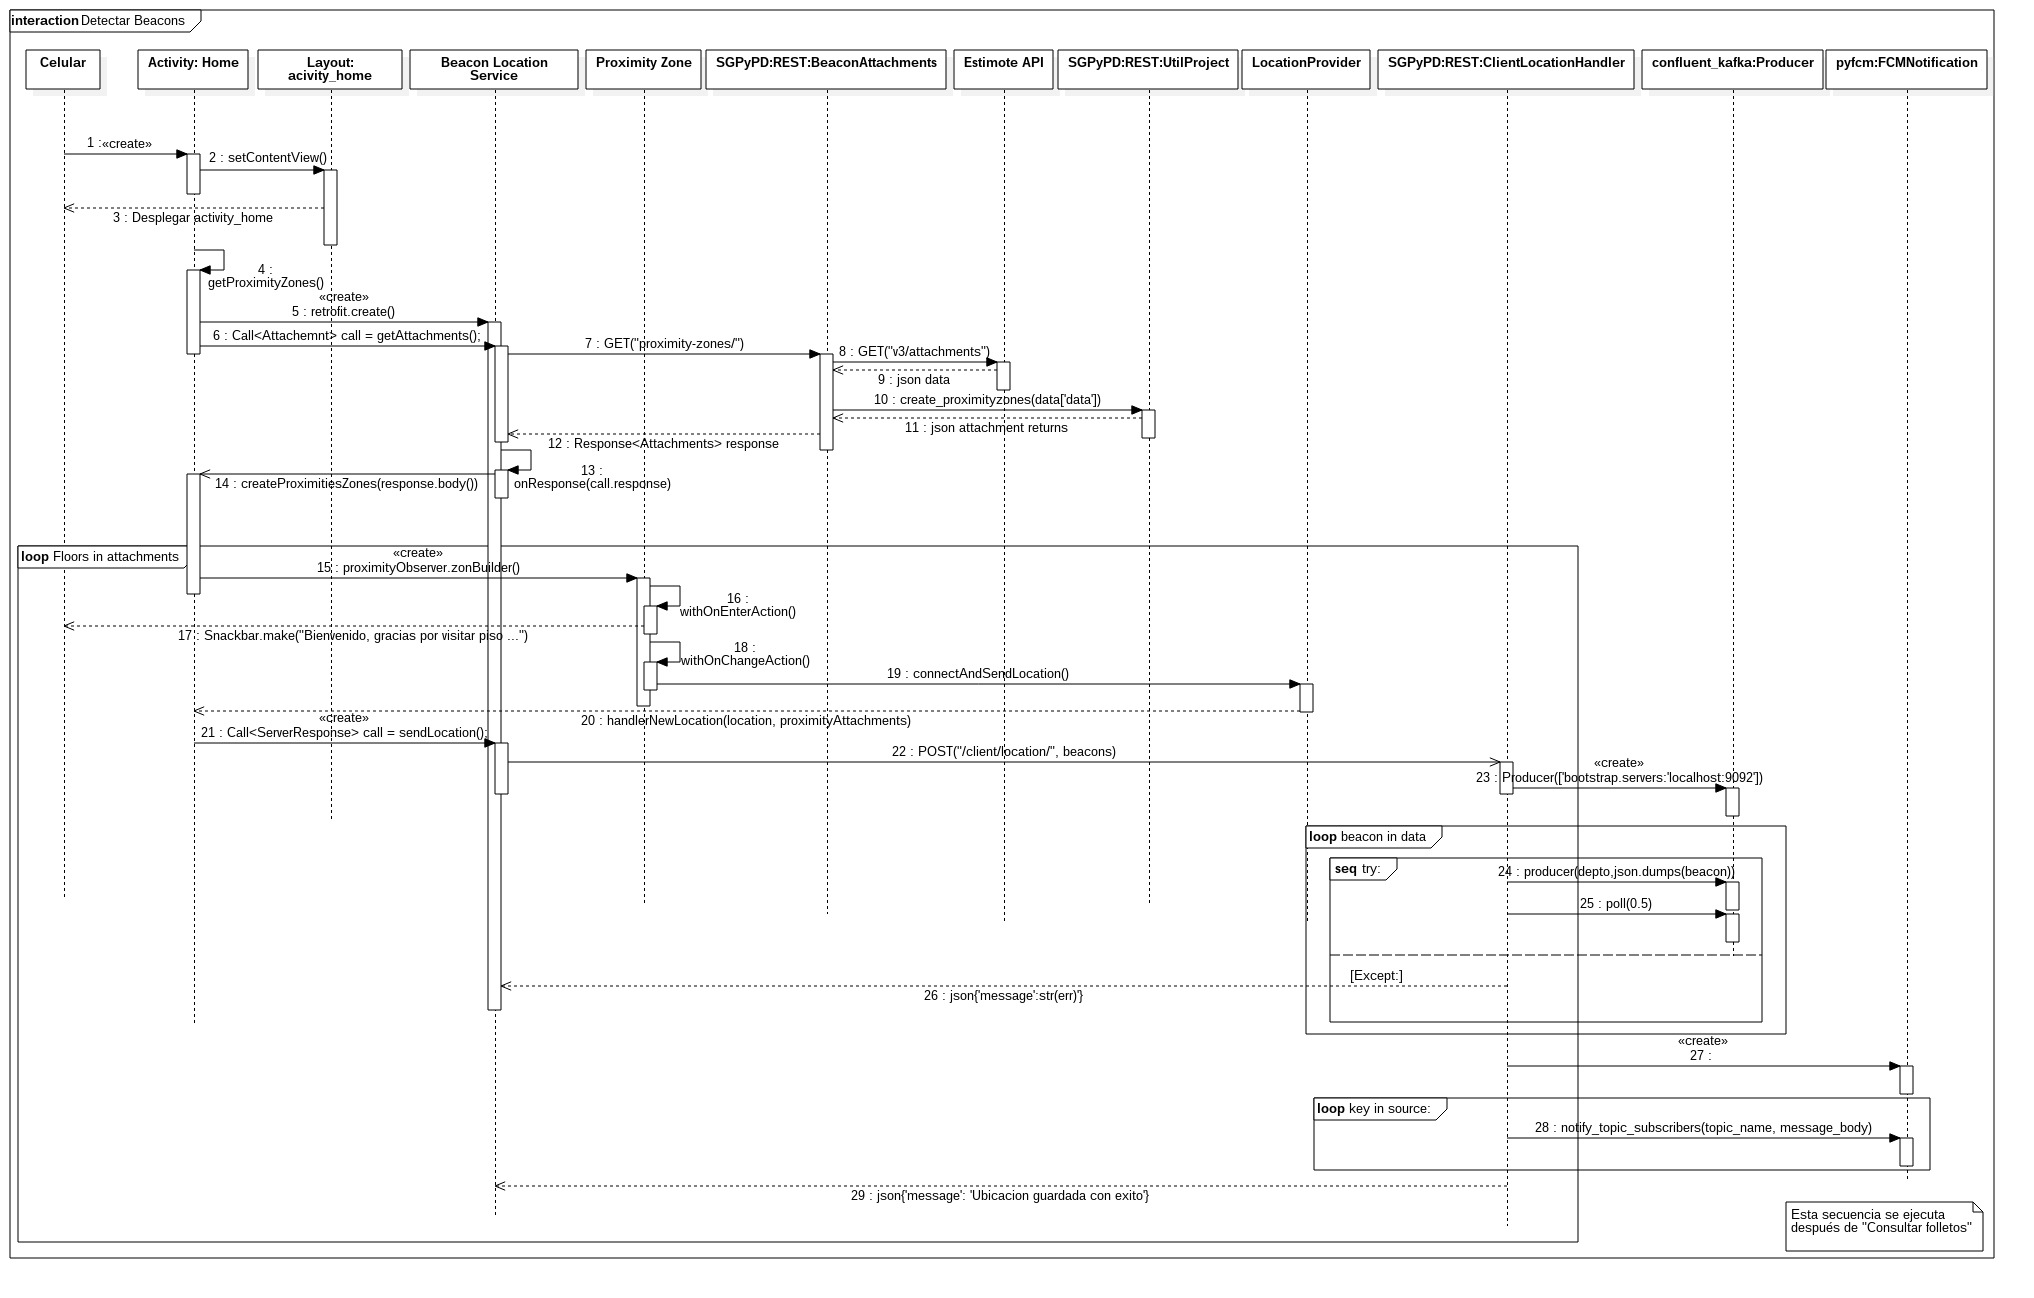
\includegraphics[width=1.1 \textwidth]{imagenes/Diagramas_UserApp/Nuevos_diagramas/detectarBeacons2}
		\caption{Diagrama de secuencia para detectar Beacons (Visualización completa).}
		\label{image:detecta2}
\end{figure}
\FloatBarrier

\FloatBarrier
\begin{figure}[htbp!]
		\centering
			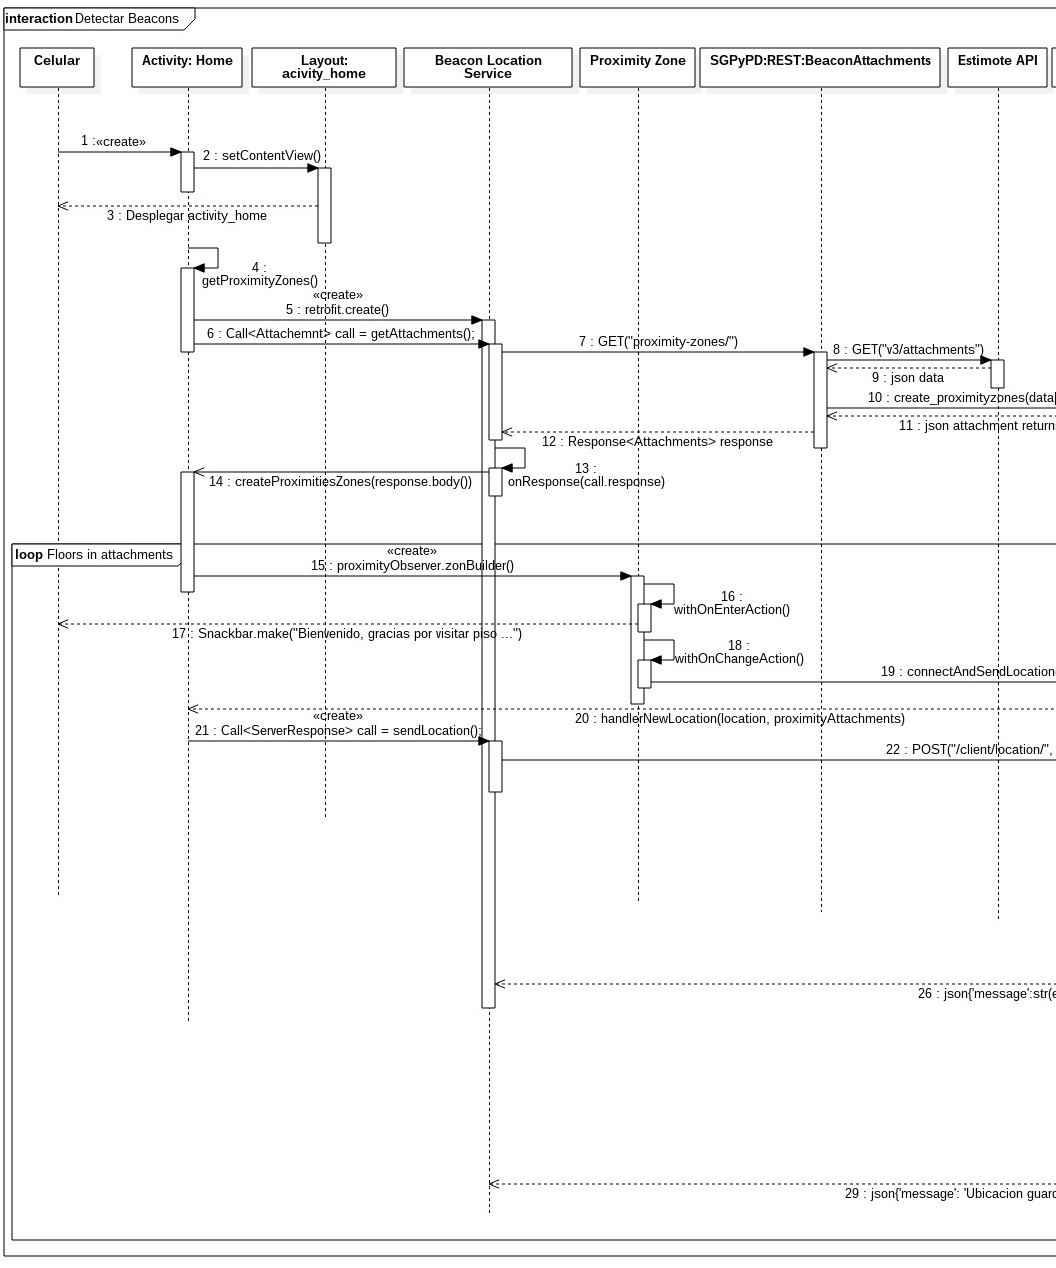
\includegraphics[width=1 \textwidth]{imagenes/Diagramas_UserApp/Nuevos_diagramas/detectarBeacons2P1}
		\caption{Diagrama de secuencia para detectar Beacons (Parte 1).}
		\label{image:detecta21}
\end{figure}
\FloatBarrier

\FloatBarrier
\begin{figure}[htbp!]
		\centering
			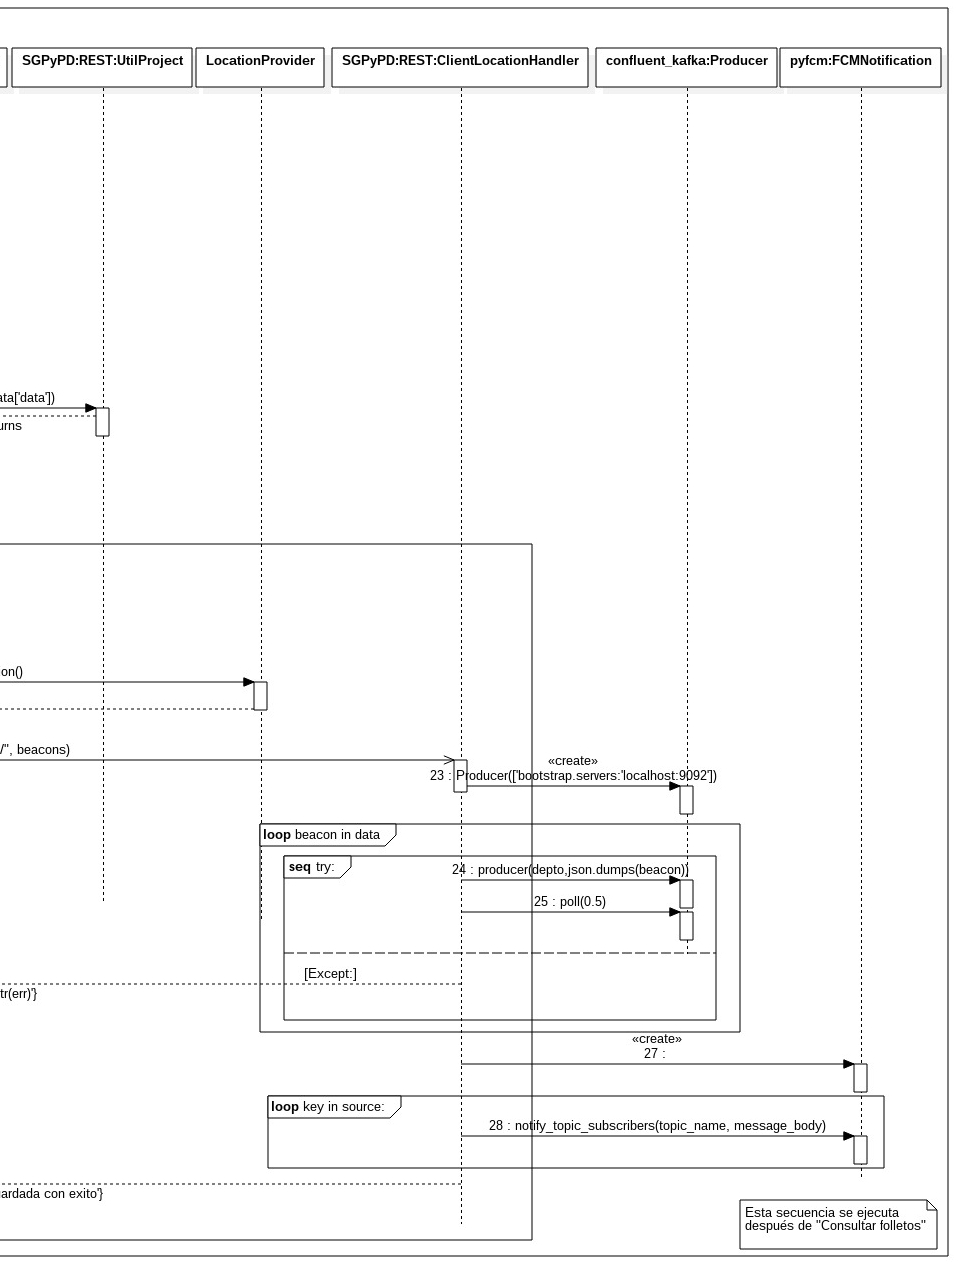
\includegraphics[width=.9 \textwidth]{imagenes/Diagramas_UserApp/Nuevos_diagramas/detectarBeacons2P2}
		\caption{Diagrama de secuencia para detectar Beacons (Parte 2).}
		\label{image:detecta22}
\end{figure}
\FloatBarrier

\subsection{Prototipo 3: Integración de módulos del sistema}
\subsubsection{Análisis}
\hypertarget{analisis}{}
Dentro de este prototipo se realiza la inclusión de todos los servicios propuestos en los requerimientos funcionales definidos previamente en el capítulo del ``Bosquejo general de la aplicación''  con el título de \hyperlink{RFAIDP}{``Requerimientos Funcionales de Aplicación Interactiva Difusora de Productos''}, sin embargo, se añadieron los requerimientos siguientes:\\
\begin{itemize}
\item Registrar cuenta nueva.
\item Recuperar contraseña. 
\item Eliminar producto de favoritos.
\item Mostrar información de productos.
\end{itemize}

\hypertarget{NRFAIDP}{}
\begin{FRequirements}
\FRitem{RFAIDP16}{Registrar cuenta nueva}{El cliente podrá crear una cuenta nueva a partir del ingreso de datos solicitados en el formulario como:
\begin{itemize}
\item Nombre,
\item Apellido paterno,
\item Apellido materno,
\item Correo electrónico,
\item Contraseña,
\item Estado civil,
\item Fecha de nacimiento.
\end{itemize}
}

\FRitem{RFAIDP17}{Recuperar contraseña}{En caso de olvidar su contraseña, el cliente podrá solicitar que le sea enviada al correo electrónico que introduzca.
}

\FRitem{RFAIDP18}{Eliminar producto de favoritos}{En caso de que el cliente haya añadido un producto a la sección de favoritos y no lo desee más, tendrá la opción de eliminar dicho producto de esta sección al presionar sobre algún producto en particular.
}

\FRitem{RFAIDP19}{Mostrar información de productos}{Si el cliente presiona sobre un artículo en particular se desplegará una nueva ventana con la información de dicho producto e imágenes de este.
}

\caption{Requerimientos añadidos a los Requerimientos Funcionales de la Aplicación Interactiva Difusora de Productos.}

\end{FRequirements}

La figura \ref{image:casosdeusoAIDP} muestra todos los casos de uso de la Aplicación Interactiva Difusora de Productos incluyendo los mencionados anteriormente.
\newpage
\title{\textbf{Casos de uso de AIDP}\\ \par}

\FloatBarrier
\begin{figure}[htbp!]
		\centering
			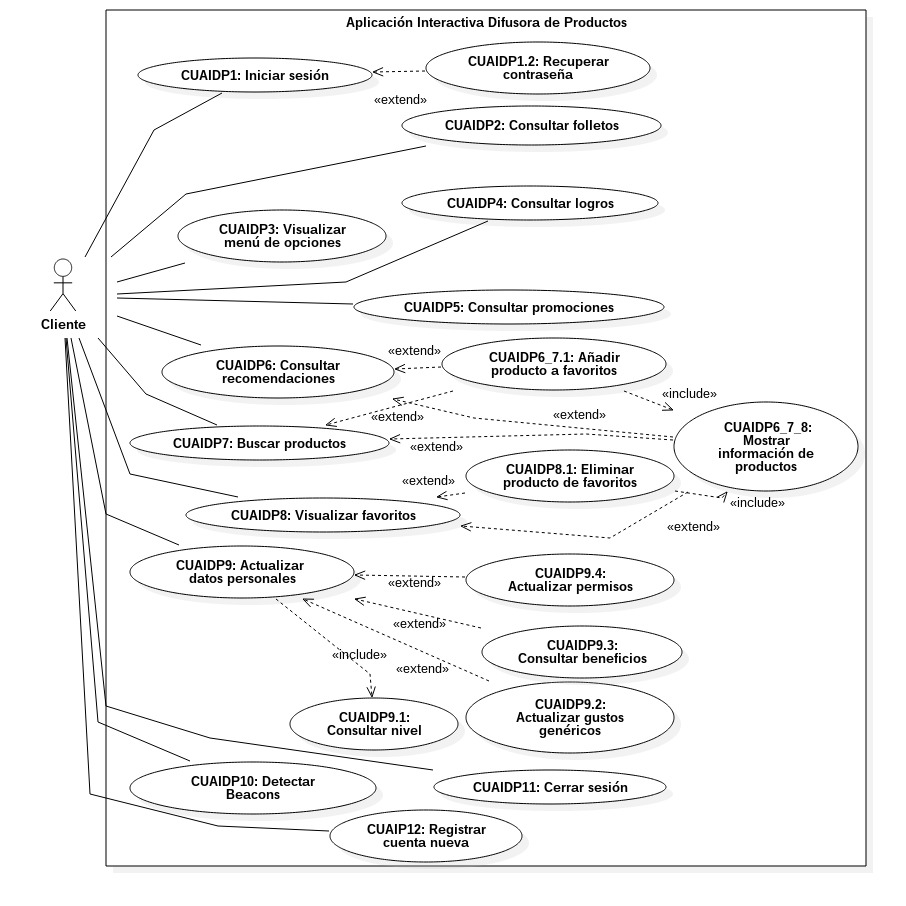
\includegraphics[width=1.1 \textwidth]{imagenes/Diagramas_UserApp/casosDeUso}
		\caption{Casos de uso de la Aplicación Interactiva Difusora de Productos.}
		\label{image:casosdeusoAIDP}
\end{figure}
\FloatBarrier

\title{\textbf{Diagrama  de clases}\\ \par}
En esta sección se muestran las clases utilizadas para este prototipo y de las cuales se hacen uso para el la implementación de los diagramas de secuencia.\\
Las primeras figuras mostradas a continuación, son las clases POJO (por sus siglas en inglés Plain Old Java Object), las cuales en los diagramas posteriores, se podrá visualizar la dependencia que estas tienen con respecto a otras clases, sin embargo debido al tamaño de los diagramas, se optó por mostrar por separado los atributos y métodos de estas clases para una mejor visualización.
\\ \par
\textit{Nota: Es importante mencionar que estas clases al ser POJO son únicamente utilizadas como medio para la obtención y transformación de los datos que son recibidos desde el sistema de gestión, procesamiento y proveedor de datos de Retail, a un formato nativo de Java.}
\FloatBarrier
\begin{figure}[htbp!]
		\centering
			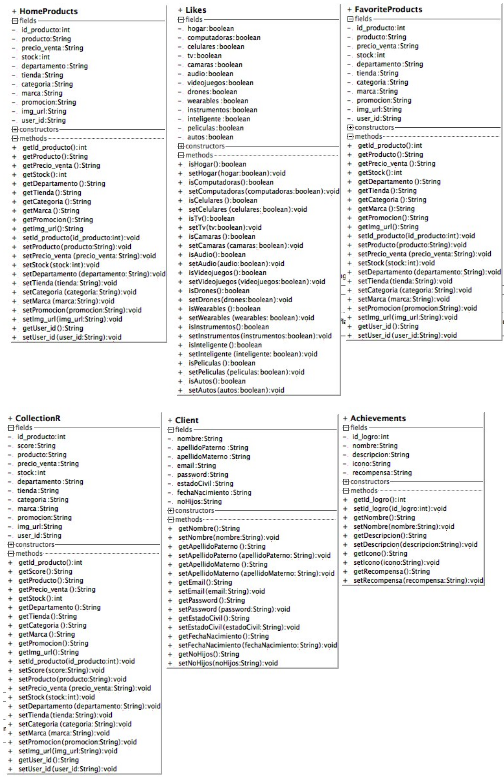
\includegraphics[width=.63 \textwidth]{imagenes/aidp_clases/pojo1n}
		\caption{Clases POJO (Parte 1).}
		\label{image:pojo1}
\end{figure}
\FloatBarrier
\FloatBarrier
\begin{figure}[htbp!]
		\centering
			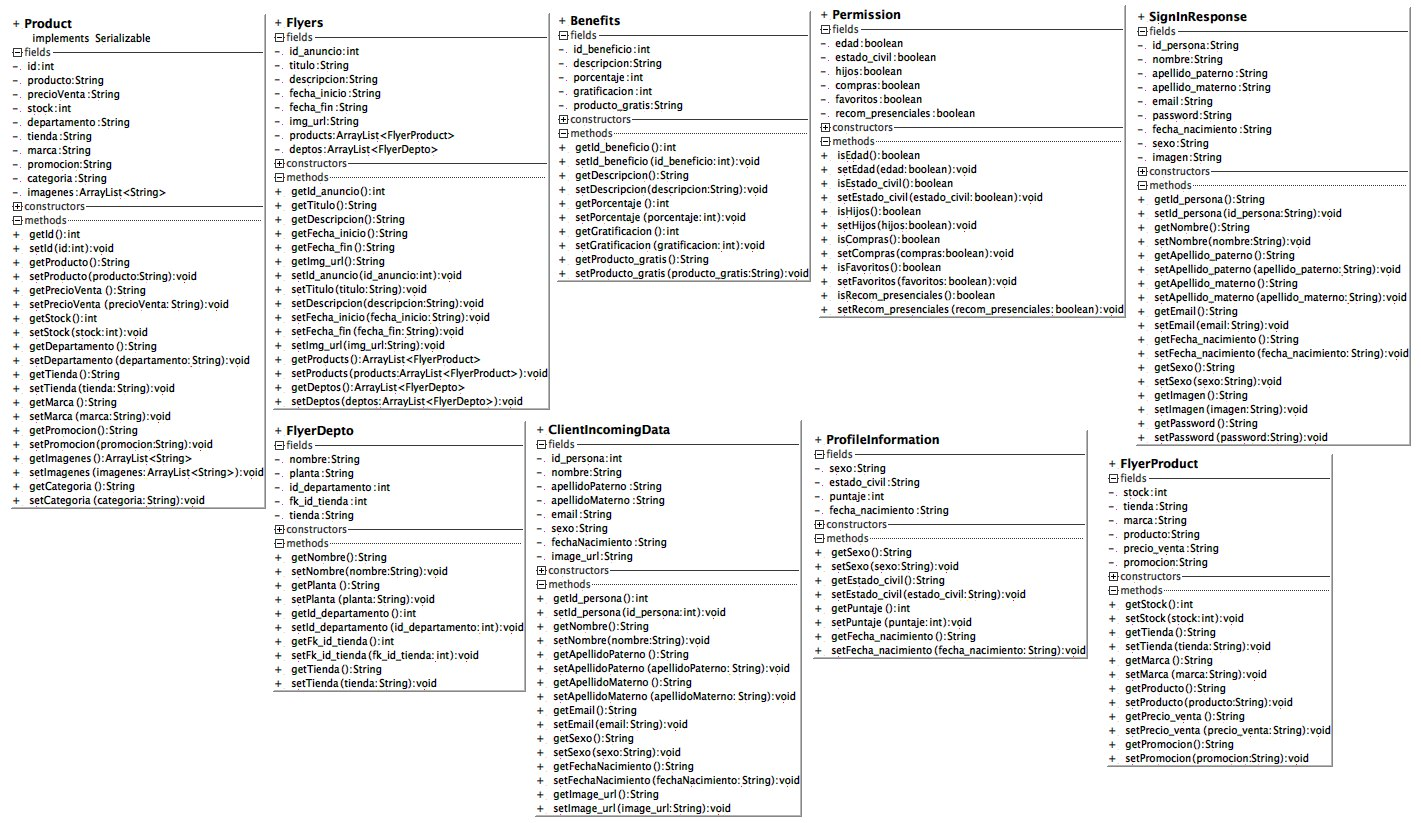
\includegraphics[width=1.1 \textwidth]{imagenes/aidp_clases/pojo2}
		\caption{Clases POJO (Parte 2).}
		\label{image:pojo2}
\end{figure}
\FloatBarrier
\FloatBarrier
\begin{figure}[htbp!]
		\centering
			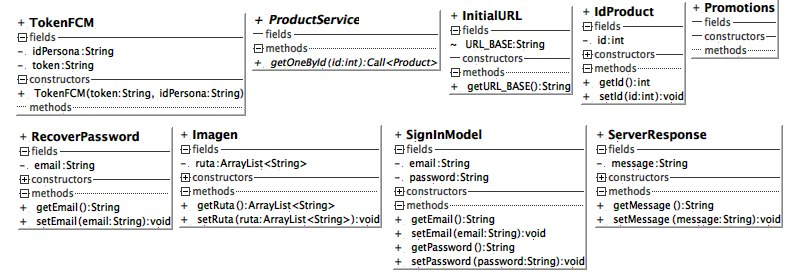
\includegraphics[width=1.1 \textwidth]{imagenes/aidp_clases/pojo3}
		\caption{Clases POJO (Parte 3).}
		\label{image:pojo3}
\end{figure}
\FloatBarrier
\FloatBarrier
\begin{figure}[htbp!]
		\centering
			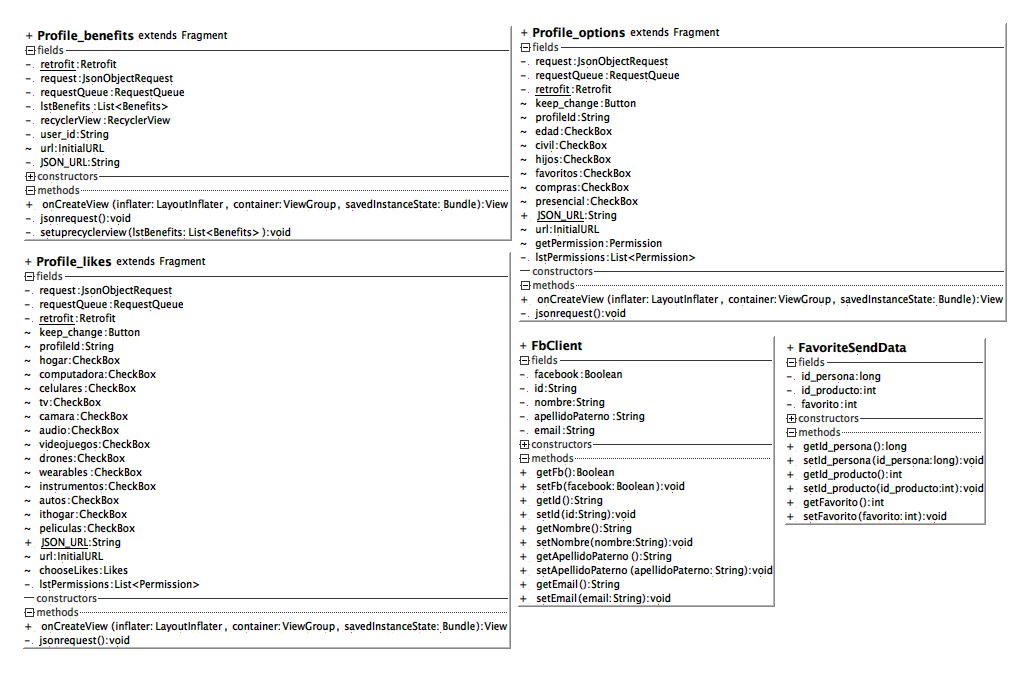
\includegraphics[width=1.1 \textwidth]{imagenes/aidp_clases/pojo4}
		\caption{Clases POJO (Parte 4).}
		\label{image:pojo4}
\end{figure}
\FloatBarrier
Los diagramas de la figura \ref{image:recycler2} y \ref{image:recycler3}, muestran las clases atributos y métodos de las clases que ya se han plasmado en el diagrama de la figura \ref{image:recycler1}, esto se realiza con el fin de una mejor visualización de las clases mencionadas.
\FloatBarrier
\begin{figure}[htbp!]
		\centering
			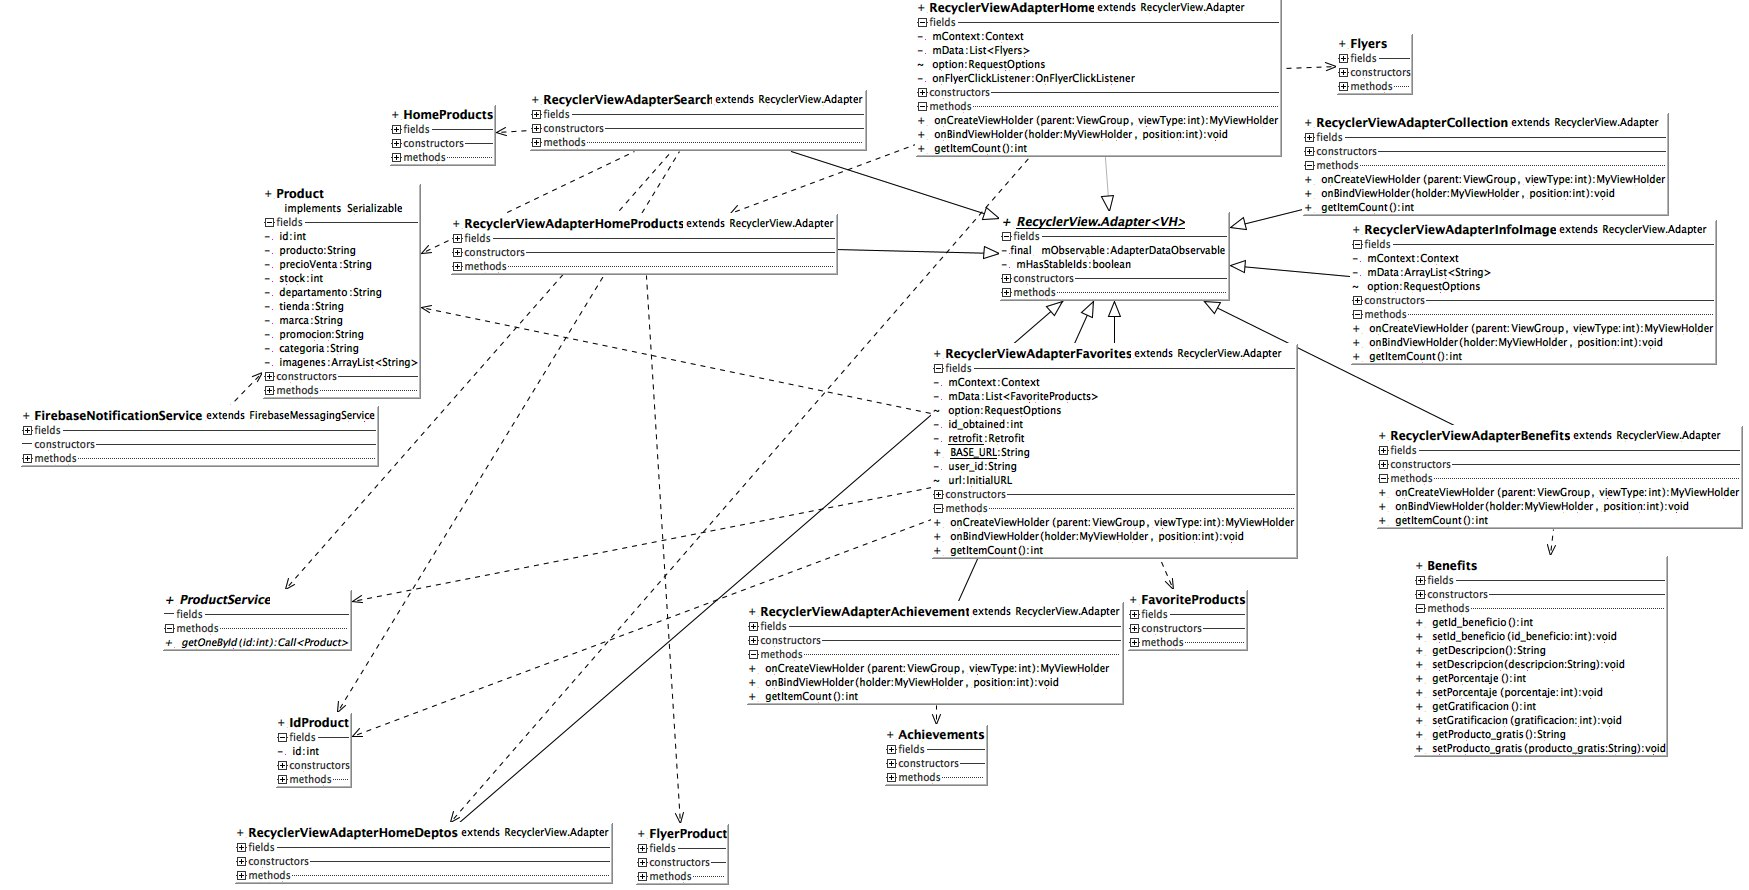
\includegraphics[width=1.1 \textwidth]{imagenes/aidp_clases/recycler1}
		\caption{Diagrama de clases del prototipo 2 de la AIDP (Visualización completa).}
		\label{image:recycler1}
\end{figure}
\FloatBarrier

\FloatBarrier
\begin{figure}[htbp!]
		\centering
			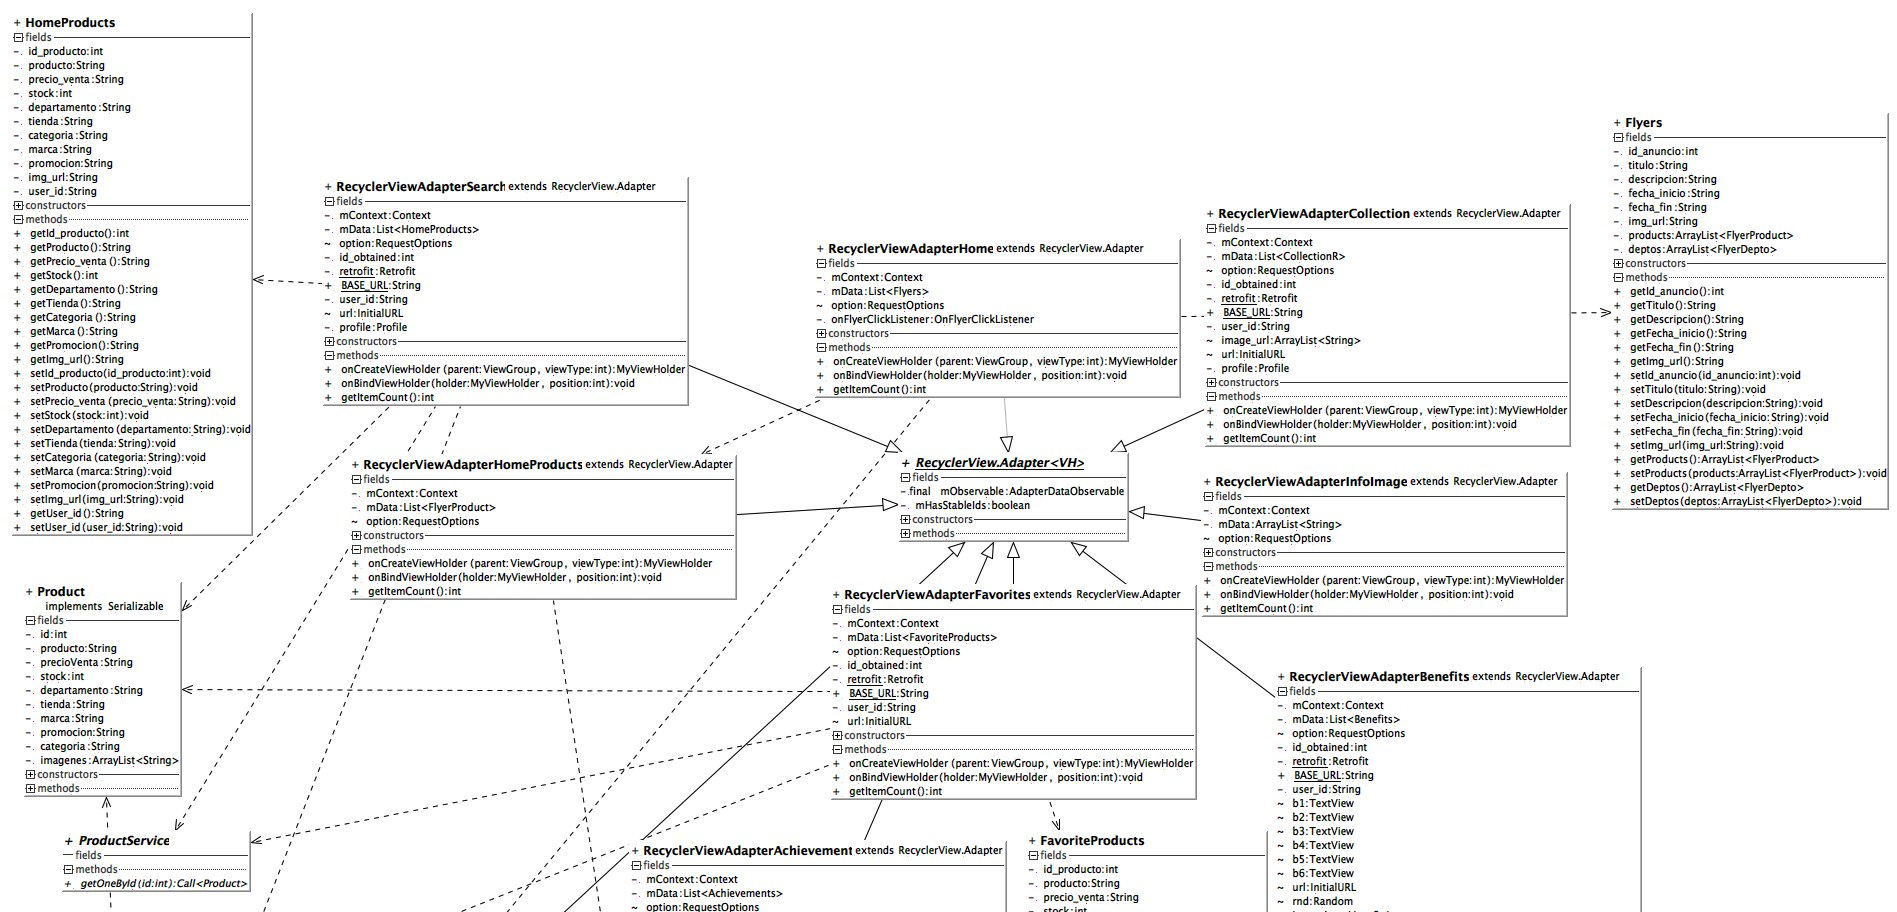
\includegraphics[width=1.1 \textwidth]{imagenes/aidp_clases/recycler2}
		\caption{Diagrama de clases del prototipo 2 de la AIDP (Parte 1).}
		\label{image:recycler2}
\end{figure}
\FloatBarrier

\FloatBarrier
\begin{figure}[htbp!]
		\centering
			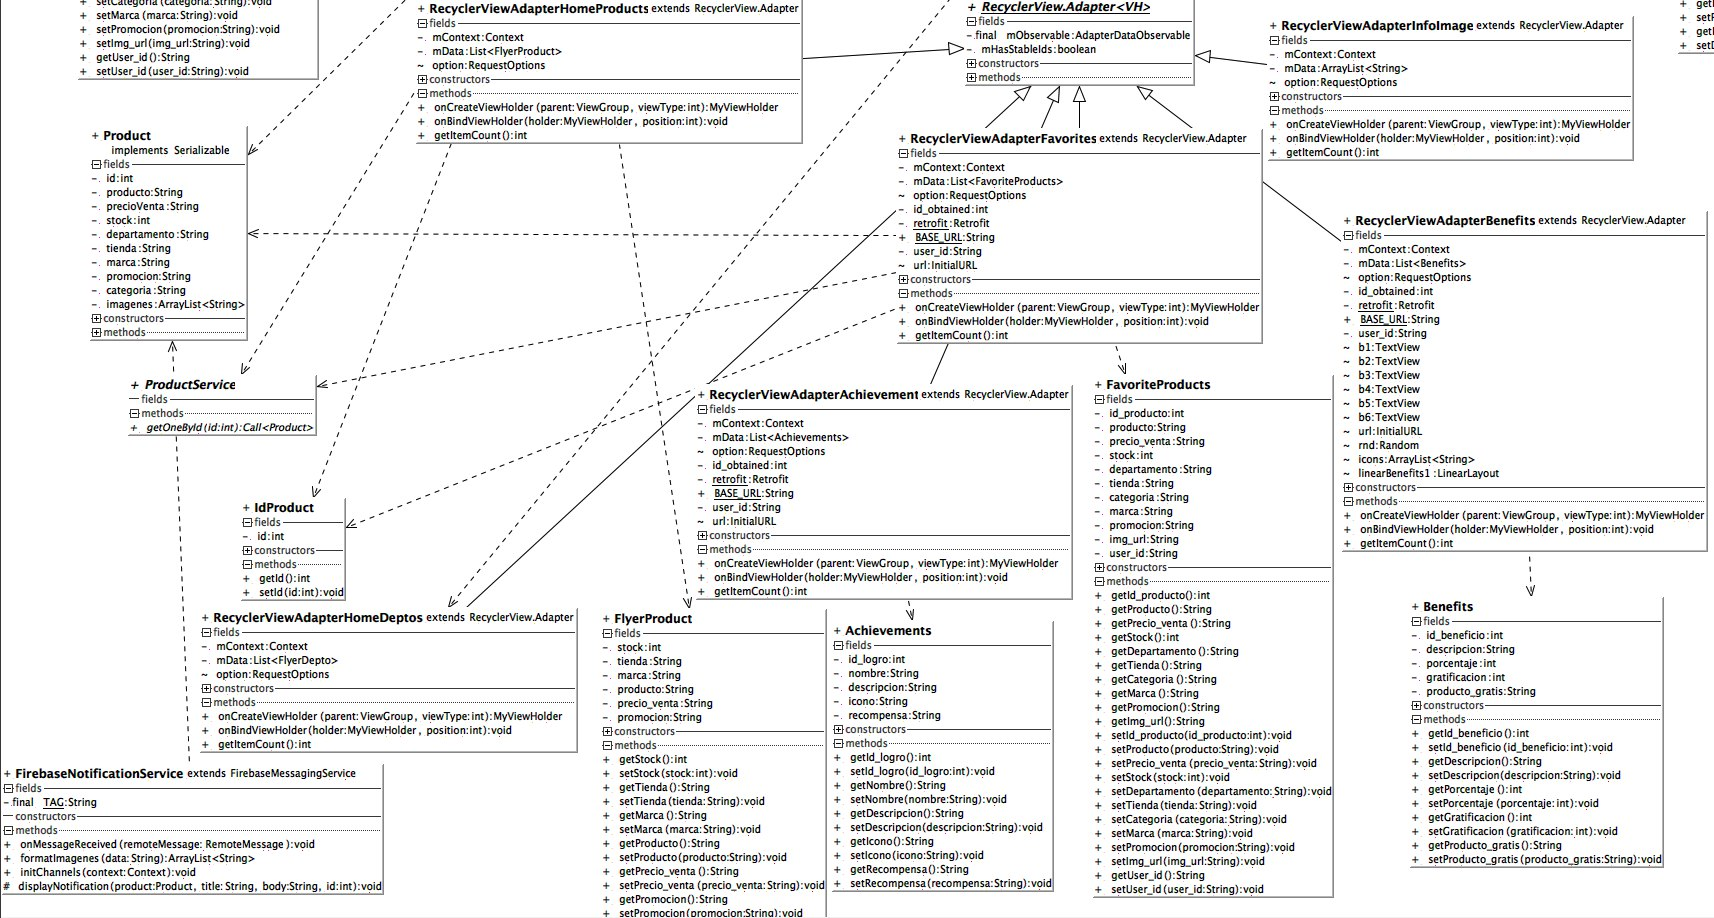
\includegraphics[width=1.1 \textwidth]{imagenes/aidp_clases/recycler3}
		\caption{Diagrama de clases del prototipo 2 de la AIDP (Parte 2)}
		\label{image:recycler3}
\end{figure}
\FloatBarrier
La descripción de los elementos de la parte 1 del diagrama de clases es la siguiente: 

\begin{itemize}
\item \textbf{RecyclerView.Adapter}: Clase encargada de transformar los modelos de datos a objetos que entienda el componente visual.
\\ \par 
Las clases enlistadas a continuación son como se muestra en el diagrama, una generalización de la clase RecyclerView.Adapter, por lo cual tienen comportamientos similares y son las encargadas de modelar los datos para su correcta visualización, dichos datos son tanto la información de un producto en particular, los productos con promociones, los departamentos con promociones o los logros y beneficios que un usuario puede tener.
\item \textbf{RecyclerViewAdapterSearch}: Datos de productos
\item \textbf{RecyclerViewAdapterHomeProducts}: Datos de productos con promociones.
\item \textbf{RecyclerViewAdapterHomeDeptos}: Datos de departamentos con promociones.
\item \textbf{RecyclerViewAdapterAchievement}: Datos de logros.
\item \textbf{RecyclerViewAdapterAdapterHome}: Datos de promociones en general.
\item \textbf{RecyclerViewAdapterCollection}: Datos de productos recomendados.
\item \textbf{RecyclerViewAdapterInfoImage}: Imágenes de productos.
\item \textbf{RecyclerViewAdapterBenefits}: Datos de beneficios.
\item \textbf{RecyclerViewAdapterFavorites}: Datos de productos almacenados como favoritos.
\end{itemize}
\newpage
El diagrama de la figura \ref{image:clases22} muestra la parte 2 del diagrama de clases.

\FloatBarrier
\begin{figure}[htbp!]
		\centering
			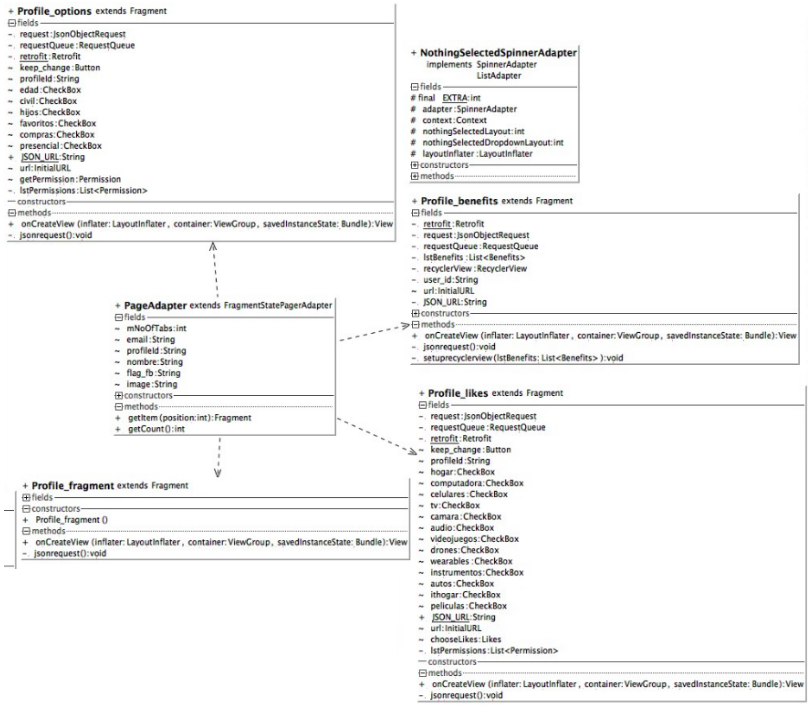
\includegraphics[width=1.1 \textwidth]{imagenes/aidp_clases/pageA}
		\caption{Diagrama de clases del prototipo 2 de la AIDP (Visualización completa).}
		\label{image:clases22}
\end{figure}
\FloatBarrier

La descripción de los elementos de la parte 2 del diagrama de clases es la siguiente: 
\begin{itemize}
\item \textbf{PageAdapter}: Clase que nos permite mostrar distintas pantallas desplazando la página actual.
\item \textbf{Profile\_options}: Clase encargada de recibir desde el sistema de gestión, procesamiento y proveedor de datos de Retail, los permisos que el usuario ha seleccionado y guardado para posteriormente desplegarlos.
\item \textbf{Profile\_benefits}: Clase encargada de recibir los beneficios que el usuario obtiene con respecto al nivel en el que se encuentre desde el sistema de gestión, procesamiento y proveedor de datos de Retail para posteriormente desplegarlos.
\item \textbf{Profile\_likes}: Clase encargada de recibir  desde el sistema de gestión, procesamiento y proveedor de datos de Retail, los gustos que el usuario ha seleccionado  y guardado para posteriormente desplegarlos.
\item \textbf{Profile\_fragment}: Clase encargada de recibir la información personal de cada usuario desde el sistema de gestión, procesamiento y proveedor de datos de Retail.
\end{itemize}

Los diagramas de las figuras \ref{image:clases33} y \ref{image:clases44} muestra la tercera y última parte del diagrama de clases.

\FloatBarrier
\begin{figure}[htbp!]
		\centering
			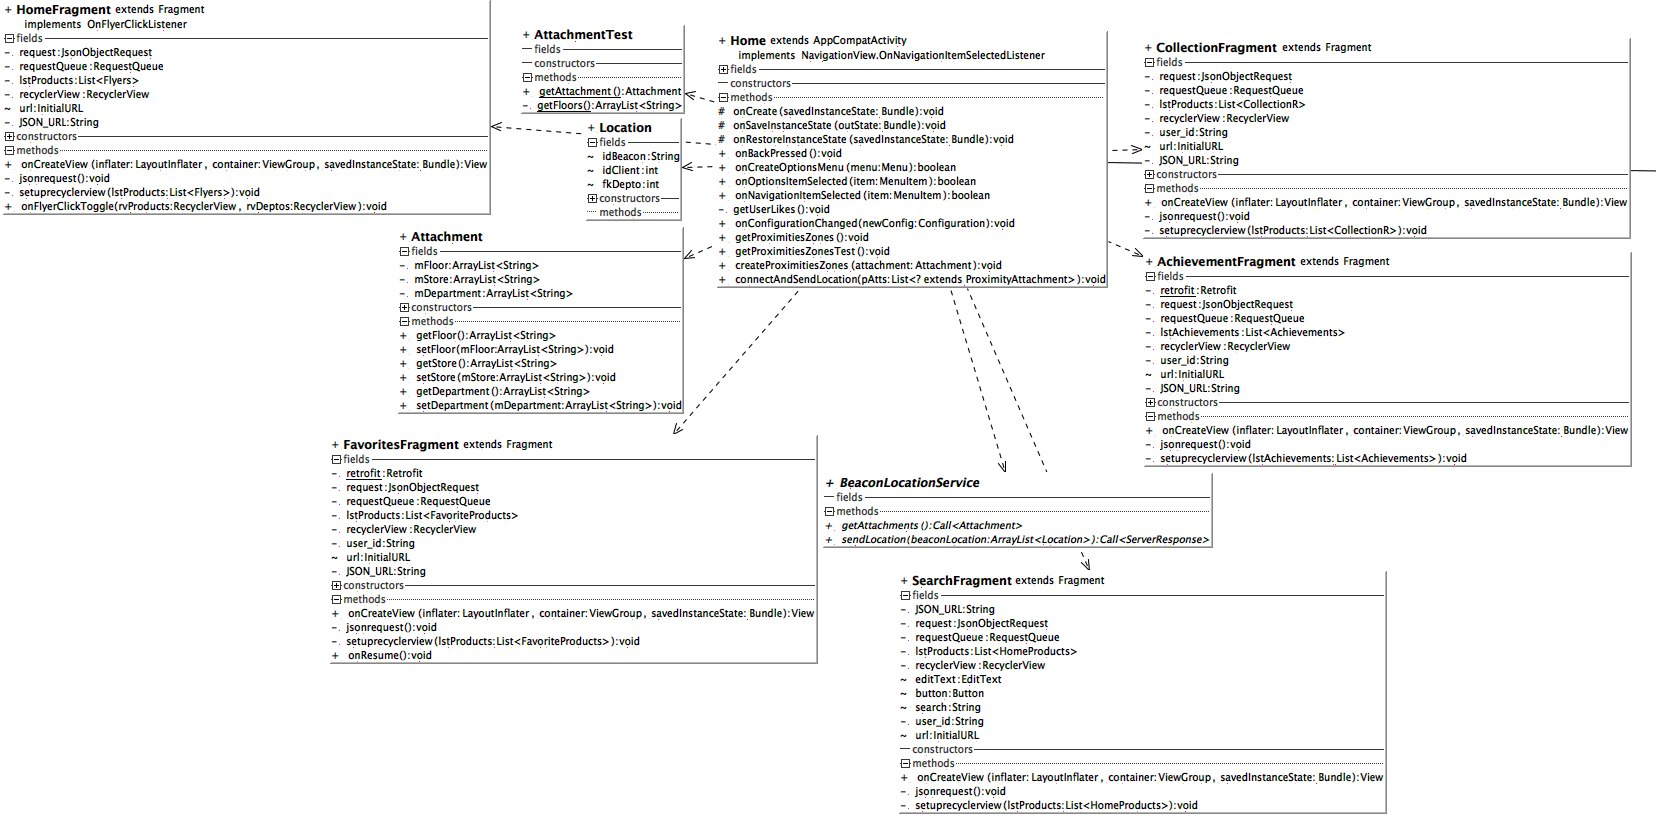
\includegraphics[width=1.1 \textwidth]{imagenes/aidp_clases/home}
		\caption{Diagrama de clases del prototipo 2 de la AIDP (Visualización completa).}
		\label{image:clases33}
\end{figure}
\FloatBarrier

La descripción de los elementos de la primera parte de la parte 3 del diagrama de clases es la siguiente: 
\begin{itemize}
\item \textbf{Home}: Clase que nos permite mostrar distintas pantallas desplazando la página actual.
\\ \par
Las clases enlistadas a continuación muestran una dependencia de la clase Home, debido a que en Home se realiza el funcionamiento del menú y este a su vez, proporciona la funcionalidad para llamar a las distintas opciones de dicho menú. Cada una de esas opciones son:
\item \textbf{HomeFragment}: Clase encargada de obtener desde el sistema de gestión, procesamiento y proveedor de datos de Retail, los folletos promocionales y productos o departamentos que igualmente cuentan con alguna promoción.
\item \textbf{CollectionFragment}: Clase encargada de obtener desde el sistema de gestión, procesamiento y proveedor de datos de Retail, los productos recomendados para cada uno de los usuarios.
\item \textbf{SearchFragment}: Clase encargada de obtener desde el sistema de gestión, procesamiento y proveedor de datos de Retail, los diferentes productos que pueden existir respecto a la búsqueda de un cliente. 
\item \textbf{FavoritesFragment}: Clase encargada de obtener desde el sistema de gestión, procesamiento y proveedor de datos de Retail, los productos que el cliente ha almacenado en su sección de favoritos.
\item \textbf{AchievementFragment}: Clase encargada de obtener desde el sistema de gestión, procesamiento y proveedor de datos de Retail, los logros que un cliente ha obtenido debido a las diferentes compras realizadas.
\\ \par 
\item \textbf{Attachment}: Clase que retrofit mapea, es la respuesta de una petición HTTP GET en formato JSON, contiene arreglos de String para generar zonas de proximidad por pisos, tiendas o departamentos.
\item \textbf{Location}: Clase que nos permite mostrar distintas pantallas desplazando la página actual.
\item \textbf{AttachmentTest}: Clase únicamente con fines de prueba para no obtener los attachments desde el servidor.
\item \textbf{BeaconLocationService}: Interfaz que define el método saveLocation para guardar la ubicación actual de Beacons y el método getAttachments que obtiene las claves - valor necesarias para generar las zonas de proximidad, esta interfaz utiliza retrofit que nos permite consumir la API REST en la aplicación.
\end{itemize}

Los diagramas de las figuras \ref{image:clases55} y \ref{image:clases66} muestran las desplegadas que previamente ya se muestran en la figura \ref{image:clases44}, esto con el fin de una mejor visualización de los atributos y métodos de cada una de ellas.

\FloatBarrier
\begin{figure}[htbp!]
		\centering
			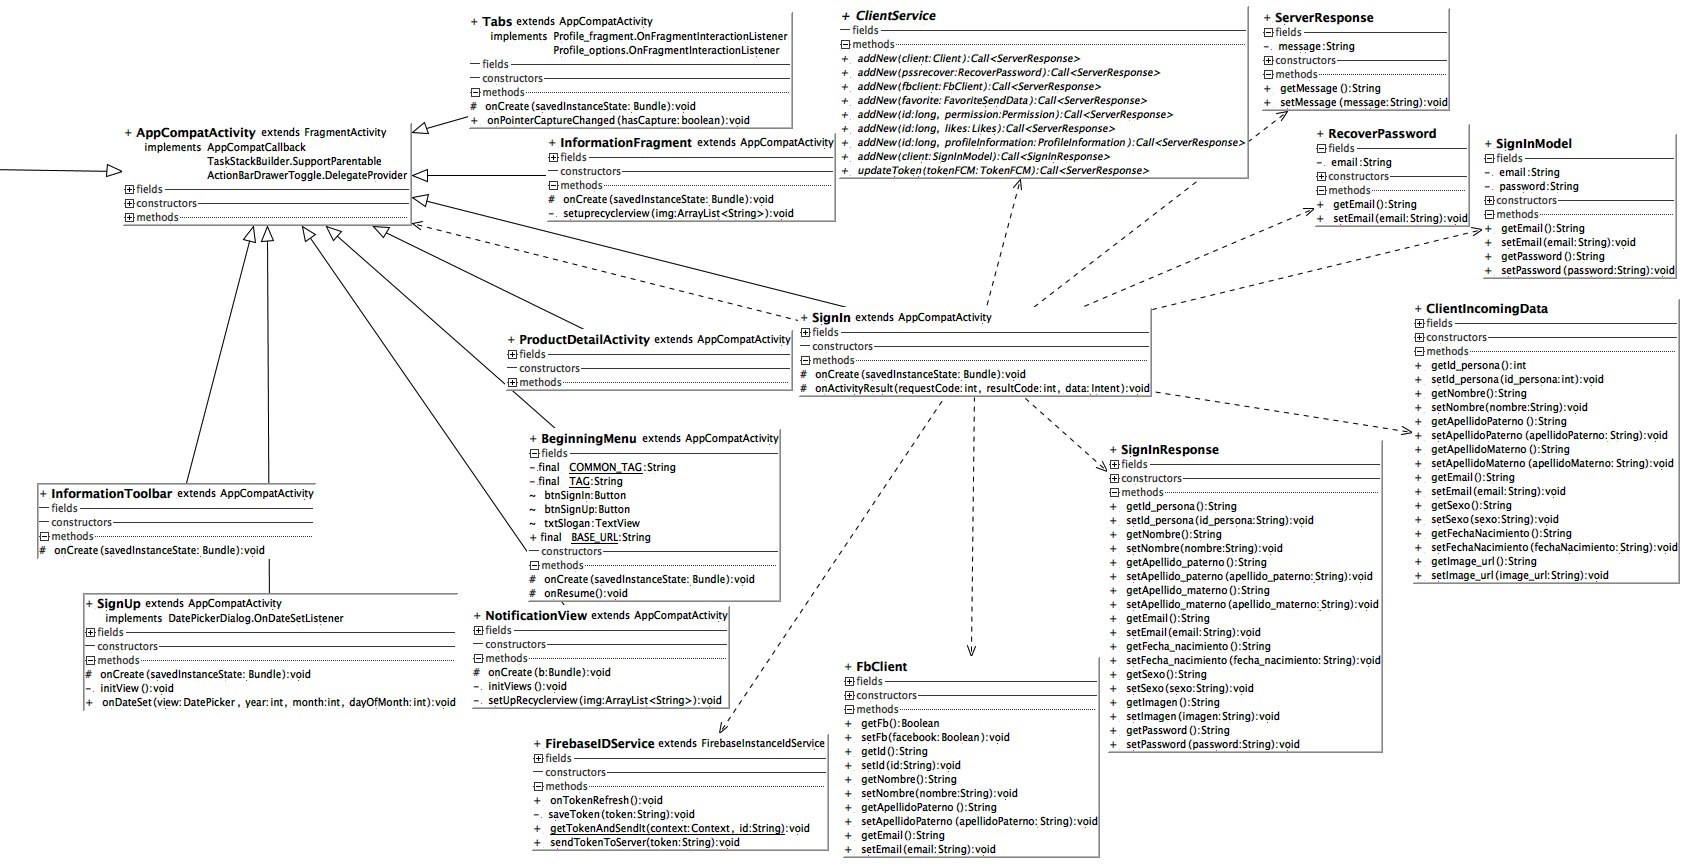
\includegraphics[width=1.1 \textwidth]{imagenes/aidp_clases/home2}
		\caption{Diagrama de clases del prototipo 2 de la AIDP (Visualización completa).}
		\label{image:clases44}
\end{figure}
\FloatBarrier

\FloatBarrier
\begin{figure}[htbp!]
		\centering
			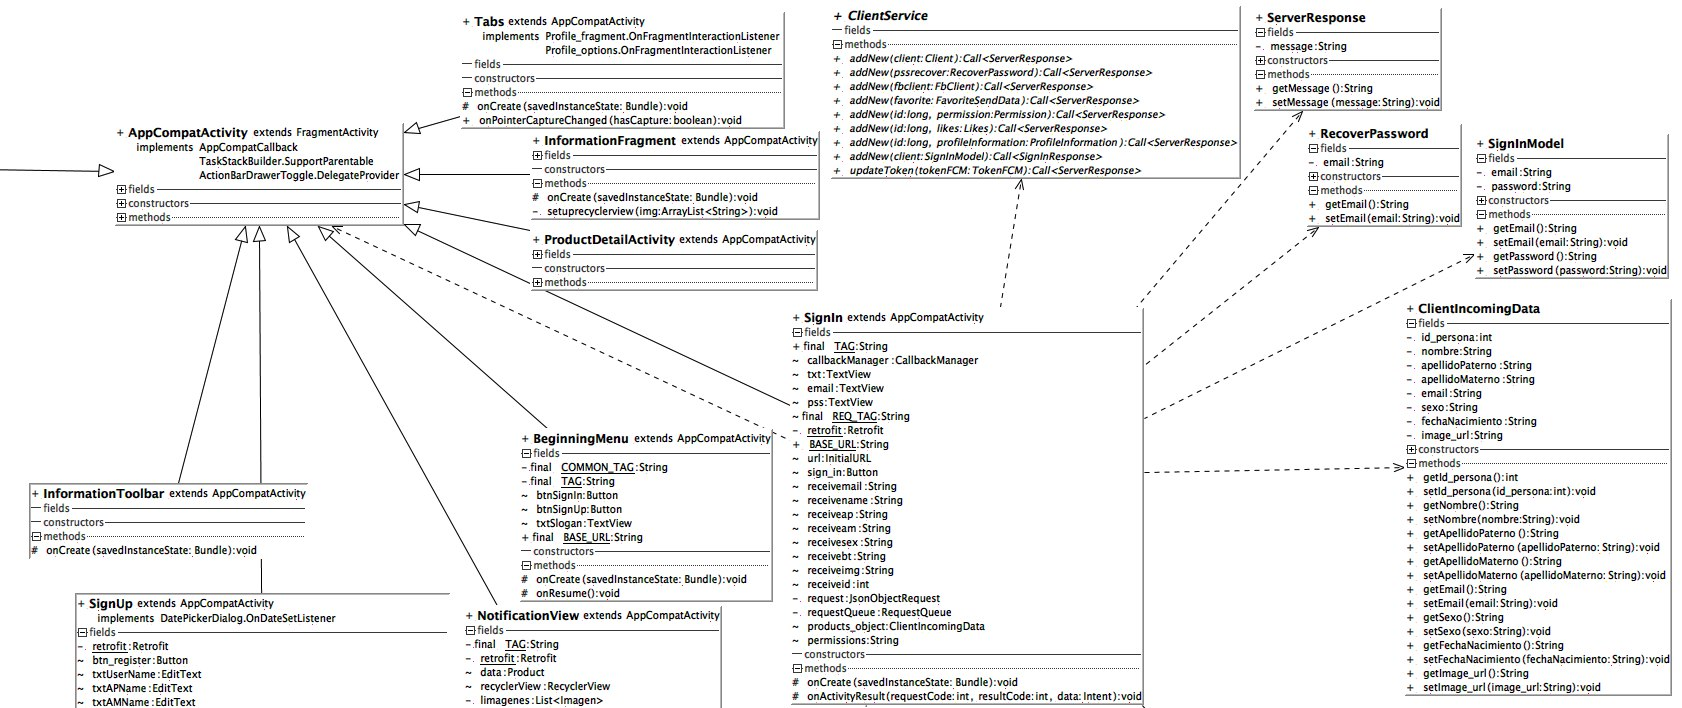
\includegraphics[width=1.1 \textwidth]{imagenes/aidp_clases/home3}
		\caption{Diagrama de clases del prototipo 2 de la AIDP (Parte 1).}
		\label{image:clases55}
\end{figure}
\FloatBarrier
\FloatBarrier
\begin{figure}[htbp!]
		\centering
			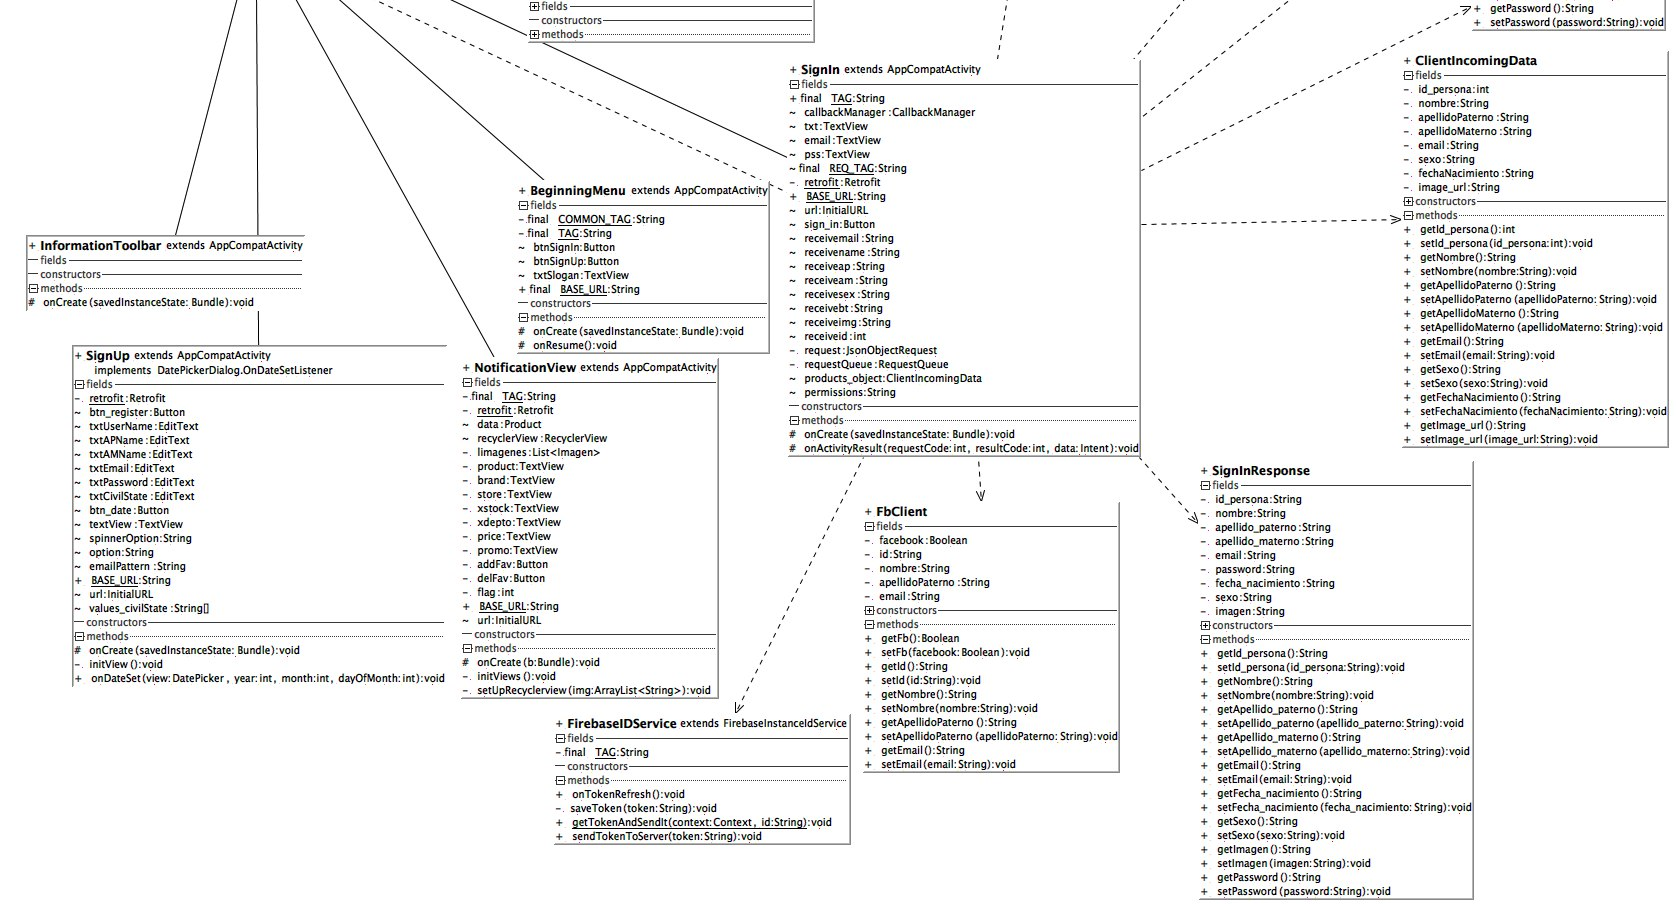
\includegraphics[width=1.1 \textwidth]{imagenes/aidp_clases/home4}
		\caption{Diagrama de clases del prototipo 2 de la AIDP (Parte 2).}
		\label{image:clases66}
\end{figure}
\FloatBarrier
La descripción de los elementos de la segunda parte de la parte 3 del diagrama de clases es la siguiente: 
\begin{itemize}
\item \textbf{AppCompatActivity}: Clase base para actividades que utilizan las características de la barra de acciones de la biblioteca de soporte de Android.
\item \textbf{SignUp}: Clase encargada de mostrar al usuario un pequeño formulario con el fin de que este registre una cuenta nueva en la aplicación.
\item \textbf{SignIn}: Clase encargada del inicio de sesión de un usuario, en dicha clase, tanto si el inicio de sesión es con una cuenta de la aplicación como si es con Facebook, se envían los datos al servidor mediante el uso de la interfaz ClientService.
\item \textbf{BegginingMenu}: Es la clase que muestra la pantalla inicial de la aplicación que únicamente es informativa.
\item \textbf{NotificationView}: Clase en donde se muestra la información de un producto que se ha recomendado y mismo que ha sido enviado al cliente mediante una notificación.
\item \textbf{ProductDetailActivity}: Clase encargada de mostrar la información de un producto en particular.
\item \textbf{Tabs}: Clase encargada de manejar las opciones que se muestran en un menú que hace uso de las clases explicadas en la parte 2 del diagrama de clases. 
\item \textbf{InformationFragment}: Clase encargada de recibir la información de un producto en particular incluyendo a su vez la obtención de un arreglo de imágenes respectivas a dicho producto.
\item \textbf{FirebaseIDService}: Clase que extiende de FirebaseInstanceIdService y funciona para obtener el token actual de Firebase Cloud Messaging para el dispositivo.
\item \textbf{ClientService}: Interfaz utilizada para hacer peticiones POST al servidor y comprobar que los datos sean correctos para un inició de sesión exitoso o para obtener la información de gustos, permisos e información de perfil de un usuario, entre otros.
\end{itemize}


\subsubsection{Diseño}
En esta sección se muestra el diseño de las pantallas de los requerimientos que fueron agregados para este prototipo mismos que se localizan en la parte superior en la sección de \hyperlink{analisis}{Análisis}. \newpage
\subparagraph{UIAIDP15 - Registrar cuenta nueva}~\\
\FloatBarrier
\IUDescripcion
[.35] % Width
{UI_userapp/cuentaNueva} % Imagen sin la ruta 'imagen/'
{UIAIDP15} % Identificador
{Registrar cuenta nueva.}  % Etiqueta/nombre de la imagen
{Registra una cuenta nueva para el caso en el que el usuario no desee ingresar con su cuenta de Facebook.} %Objetivo
{Esta pantalla (figura \ref{UIAIDP15}), nos muestra los datos requeridos para que el usuario pueda generar una cuenta nueva.} %Intro/Breve descripción de la pantalla
{Ninguna.} %Salidas
{Nombre, apellido paterno, apellido materno, correo electrónico, contraseña, estado civil y fecha de nacimiento.} %Entradas
\FloatBarrier

\subparagraph{UIAIDP16 - Recuperar contraseña} ~\\
\FloatBarrier
\IUDescripcion
[.3] % Width
{UI_userapp/recuperaContra} % Imagen sin la ruta 'imagen/'
{UIAIDP16} % Identificador
{Recuperar contraseña.}  % Etiqueta/nombre de la imagen
{En caso de que el usuario haya olvidado su contraseña, mediante un correo electrónico recupera esta.} %Objetivo
{Esta pantalla (figura \ref{UIAIDP16}), nos muestra una ventana emergente que se despliega con el fin de solicitar un correo electrónico al usuario y así enviarle esta.} %Intro/Breve descripción de la pantalla
{Ninguna.} %Salidas
{Correo electrónico.} %Entradas
\FloatBarrier

\subparagraph{UIAIDP17 - Muestra información de productos} ~\\
\FloatBarrier
\IUDescripcion
[.35] % Width
{UI_userapp/infoProdu} % Imagen sin la ruta 'imagen/'
{UIAIDP17} % Identificador
{Muestra información de productos.}  % Etiqueta/nombre de la imagen
{Proporciona la información del producto que el usuario ha seleccionado.} %Objetivo
{Esta pantalla (figura \ref{UIAIDP17}), despliega la información del producto que ha sido seleccionado por el usuario y en caso de que este contenga más imágenes aparte de la principal, las despliega. De igual manera muestra el botón para añadir un producto a la sección de Favoritos.} %Intro/Breve descripción de la pantalla
{Alerta de notificación de producto añadido a la sección de Favoritos.} %Salidas
{Ninguna.} %Entradas
\FloatBarrier

\subparagraph{UIAIDP18 - Eliminar producto de favoritos} ~\\
\FloatBarrier
\IUDescripcion
[.35] % Width
{UI_userapp/favs1} % Imagen sin la ruta 'imagen/'
{UIAIDP18} % Identificador
{Eliminar producto de favoritos.}  % Etiqueta/nombre de la imagen
{Despliega un botón que permite la eliminación de un producto de la sección de Favoritos.} %Objetivo
{Esta pantalla (figura \ref{UIAIDP18}), despliega la información del producto y de igual manera muestra un botón el cual al presionarlo elimina el producto seleccionado de la sección de Favoritos.} %Intro/Breve descripción de la pantalla
{Alerta de notificación de eliminación del producto de la sección de Favoritos.} %Salidas
{Ninguna.} %Entradas
\FloatBarrier





A continuación, se muestran los diagramas de secuencia que fueron elaborados a partir de cada uno de los módulos del sistema que fueron siendo añadidos a la AIDP. \\ \par
%SECUENCIA
\title{\textbf{Diagramas de secuencia}\\ \par}
\title{\textbf{Iniciar Sesión}}
\\ \par El diagrama de la figura \ref{image:DSIniciarsesion} se dividió en dos secciones para obtener una mejor visualización, dichas secciones corresponden a la figura \ref{image:DSIniciarsesion1} y \ref{image:DSIniciarsesion2}.
En la figura \ref{image:DSIniciarsesion} se muestra el diagrama de secuencia para iniciar sesión en la aplicación móvil, en el cual se observan las 3 diferentes alternativas mediante con las que el cliente puede iniciar sesión y acceder a la aplicación.


\FloatBarrier
\begin{figure}[htbp!]
		\centering
			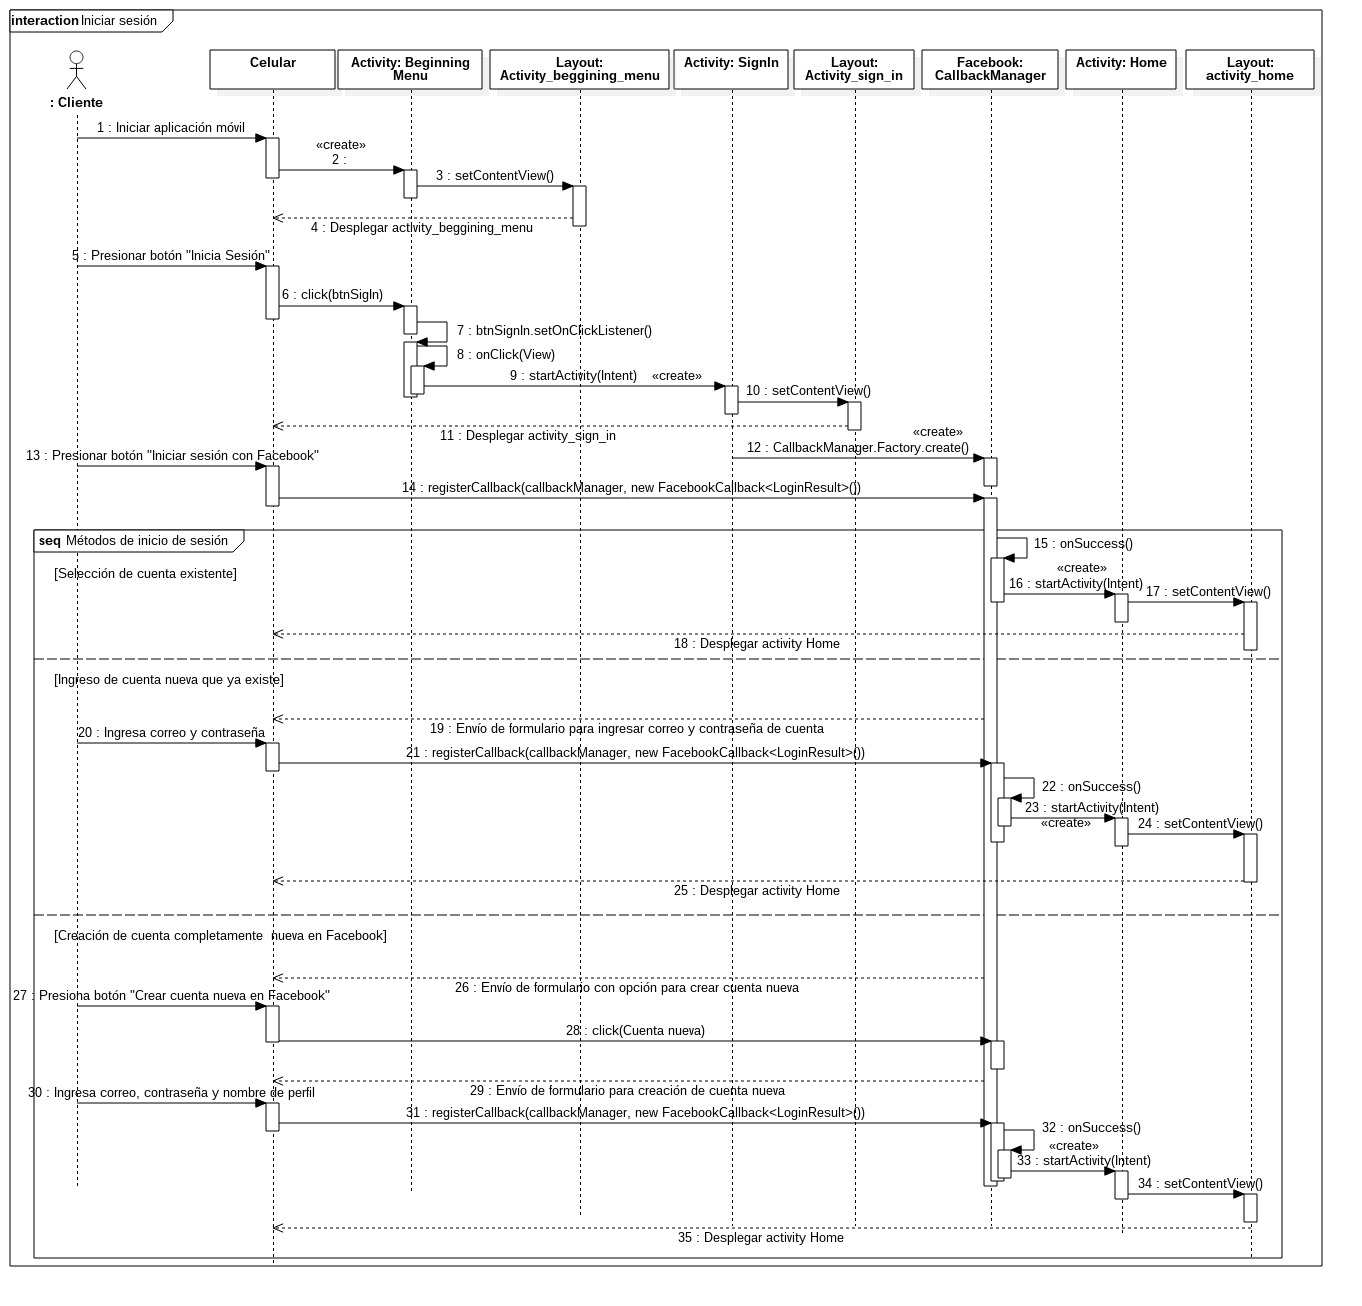
\includegraphics[width=0.9 \textwidth]{imagenes/Diagramas_UserApp/Nuevos_diagramas/IniciarSesion}
		\caption{Diagrama de secuencia para iniciar sesión (Visualización completa).}
		\label{image:DSIniciarsesion}
\end{figure}
\FloatBarrier

\FloatBarrier
\begin{figure}[htbp!]
		\centering
			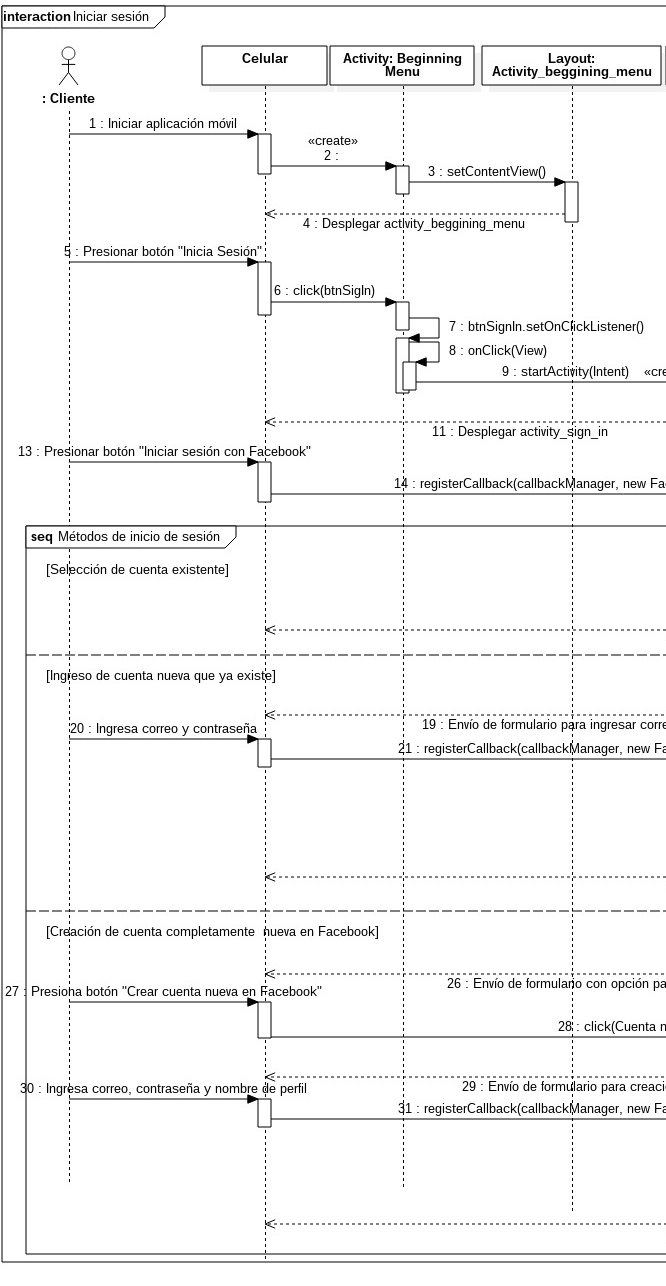
\includegraphics[width=.68 \textwidth]{imagenes/Diagramas_UserApp/Nuevos_diagramas/IniciarSesion_1}
		\caption{Diagrama de secuencia para iniciar sesión (Parte 1).}
		\label{image:DSIniciarsesion1}
\end{figure}
\FloatBarrier

\FloatBarrier
\begin{figure}[htbp!]
		\centering
			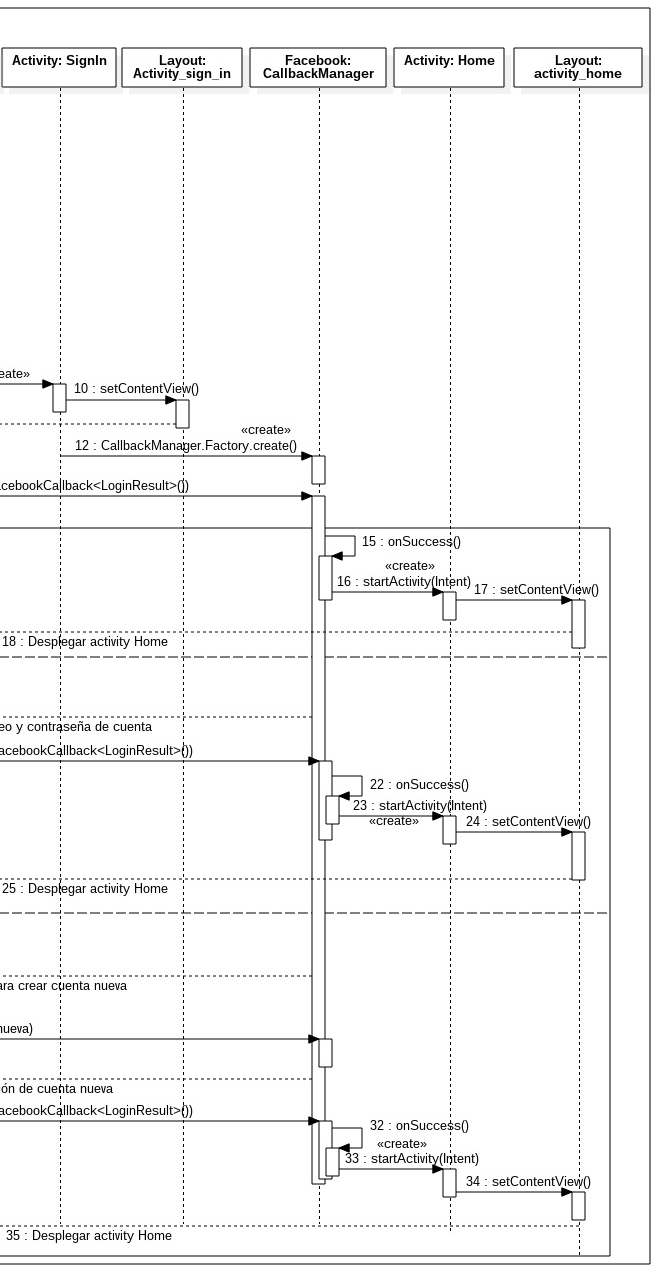
\includegraphics[width=.69 \textwidth]{imagenes/Diagramas_UserApp/Nuevos_diagramas/IniciarSesion_2}
		\caption{Diagrama de secuencia para iniciar sesión (Parte 2).}
		\label{image:DSIniciarsesion2}
\end{figure}
\FloatBarrier

\title{\textbf{Recuperar contraseña}}
\\ \par La figura \ref{image:DSRecuperaContra} se dividió en dos secciones para obtener una mejor visualización, dichas secciones corresponden a la figura \ref{image:DSIniciarsesion1} y \ref{image:DSIniciarsesion2}.
En la figura \ref{image:DSRecuperaContra} se muestra el diagrama de secuencia para recuperar la contraseña de un usuario en caso de que este no se haya registrado con Facebook en la aplicación móvil.


\FloatBarrier
\begin{figure}[htbp!]
		\centering
			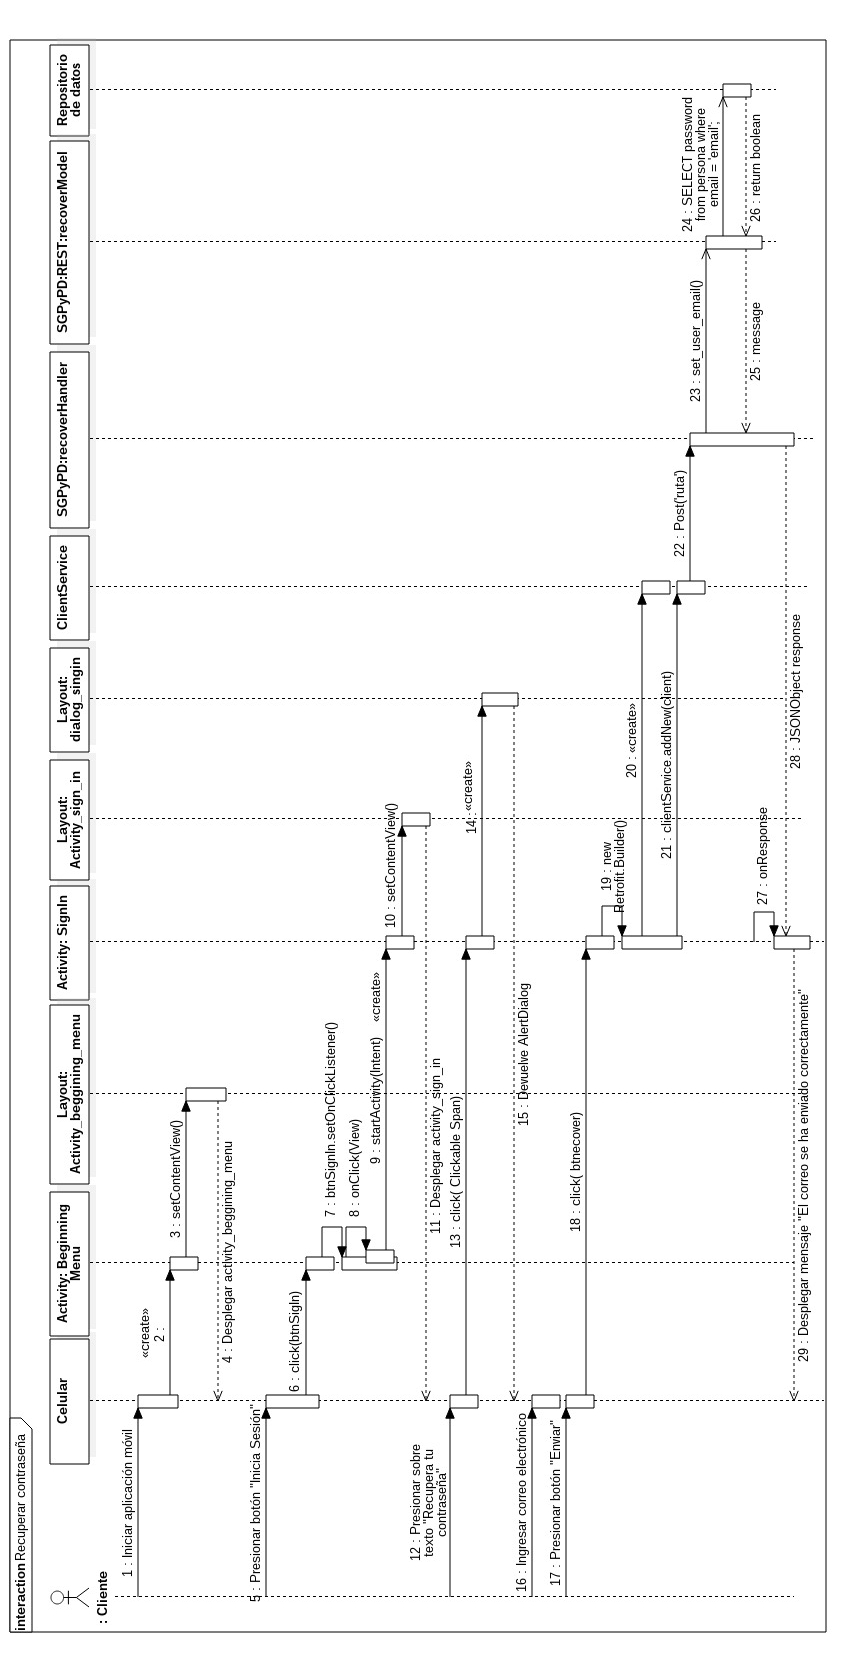
\includegraphics[width=0.57 \textwidth]{imagenes/Diagramas_UserApp/Nuevos_diagramas/Horizontal/recuperarContra}
		\caption{Diagrama de secuencia para recuperar contraseña (Visualización completa).}
		\label{image:DSRecuperaContra}
\end{figure}
\FloatBarrier

\FloatBarrier
\begin{figure}[htbp!]
		\centering
			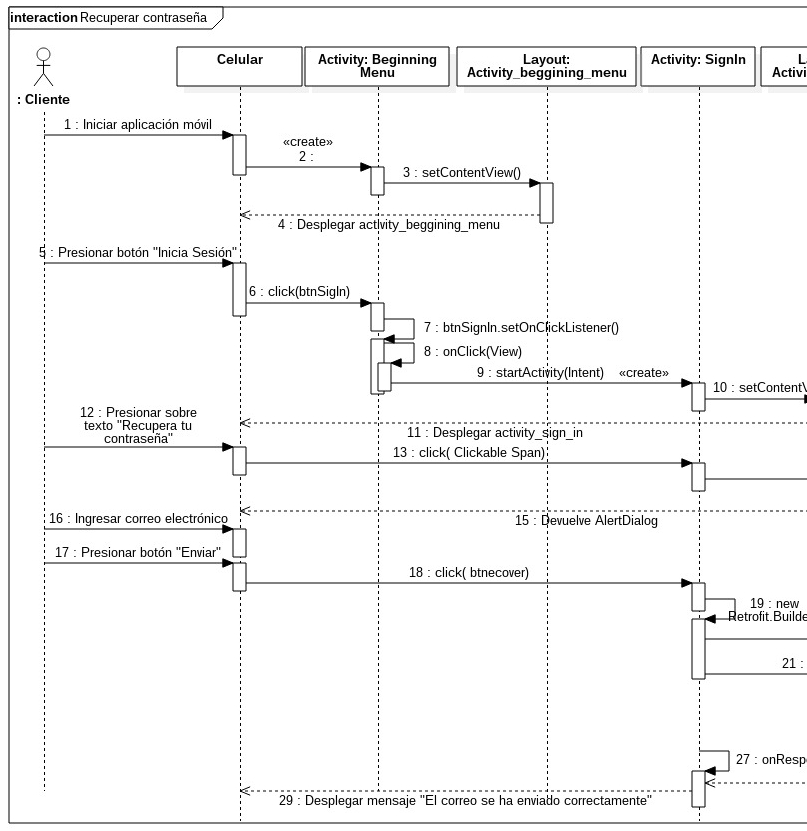
\includegraphics[width=0.9 \textwidth]{imagenes/Diagramas_UserApp/Nuevos_diagramas/recuperarContra_1}
		\caption{Diagrama de secuencia para recuperar contraseña (Parte 1).}
		\label{image:DSRecuperaContra1}
\end{figure}
\FloatBarrier

\FloatBarrier
\begin{figure}[htbp!]
		\centering
			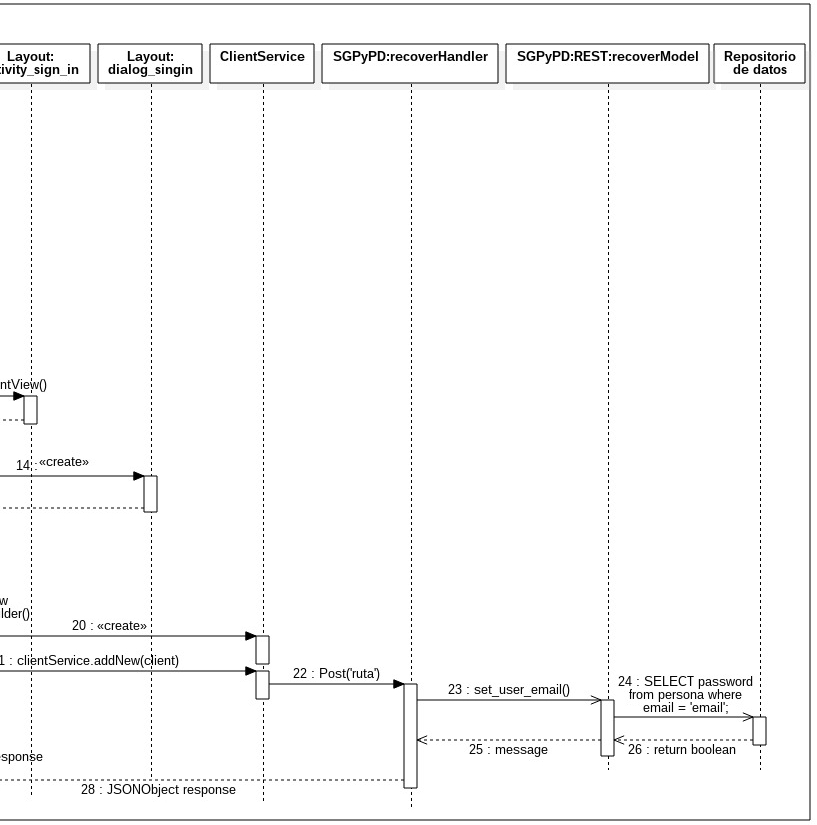
\includegraphics[width=.9 \textwidth]{imagenes/Diagramas_UserApp/Nuevos_diagramas/recuperarContra_2}
		\caption{Diagrama de secuencia para recuperar contraseña (Parte 2).}
		\label{image:DSRecuperaContra1}
\end{figure}
\FloatBarrier

\title{\textbf{Registrar cuenta nueva}}
\\ \par
El diagrama de la figura \ref{image:RegistrarCuenta} se dividió en dos secciones para obtener una mejor visualización, dichas secciones corresponden a la figura \ref{image:RegistrarCuenta1} y \ref{image:RegistrarCuenta2}. Este diagrama corresponde a la secuencia ``Registrar cuenta nueva'' mediante la cual, el usuario puede crear una cuenta en caso de que no desee iniciar sesión con Facebook.
\FloatBarrier
\begin{figure}[htbp!]
		\centering
			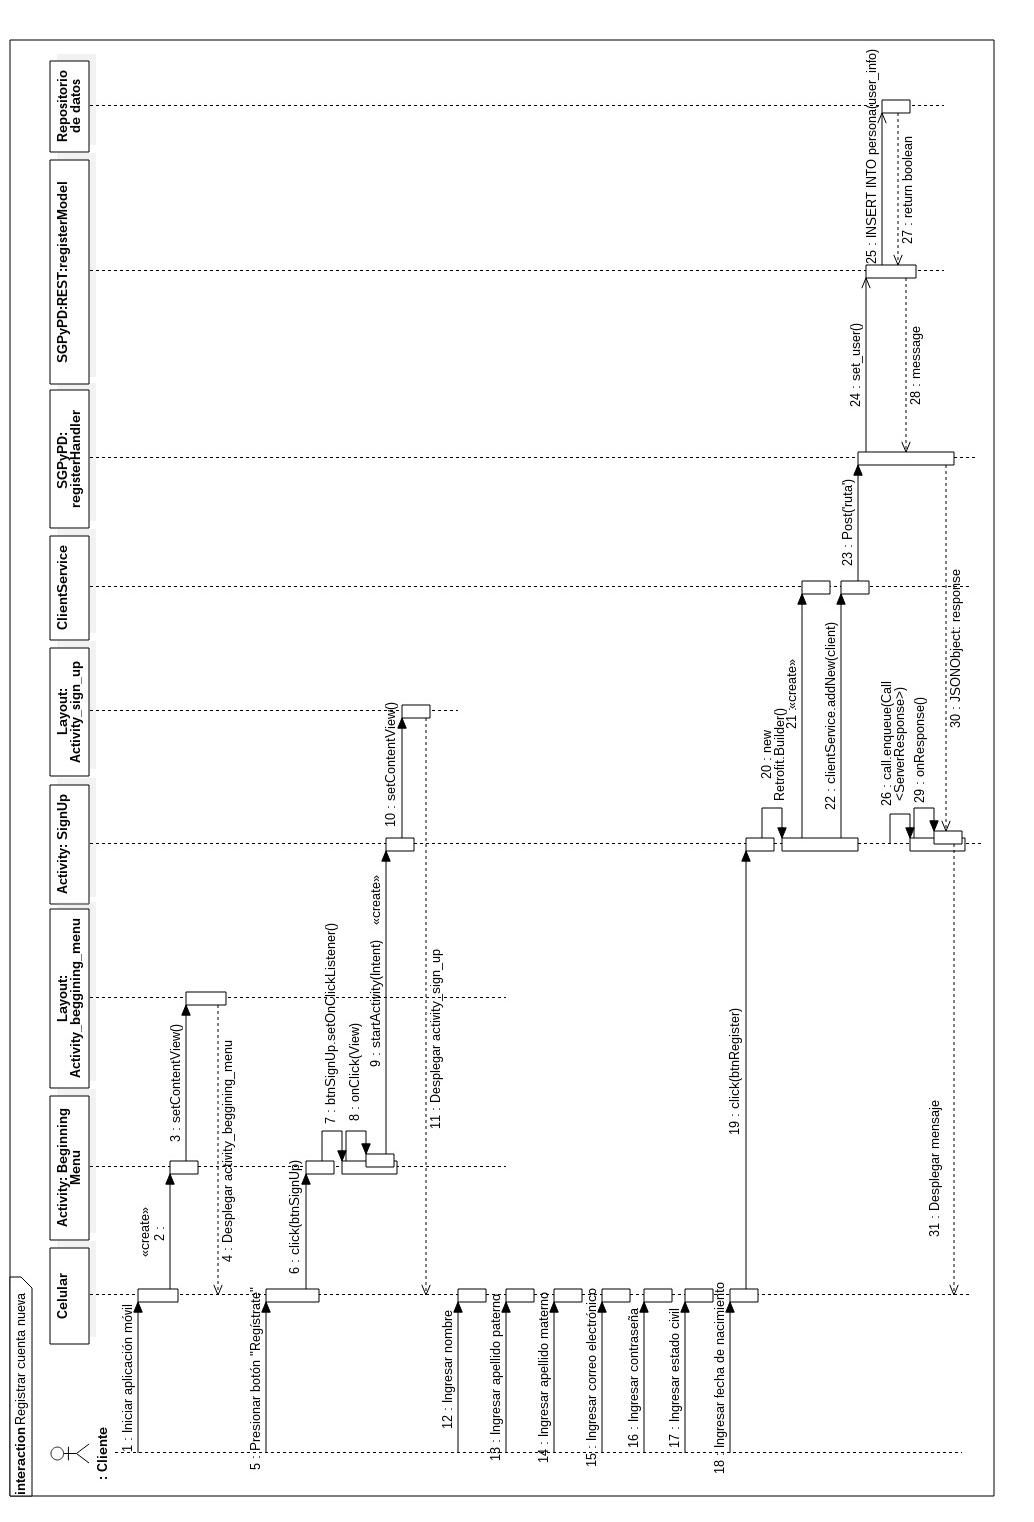
\includegraphics[width=0.9 \textwidth]{imagenes/Diagramas_UserApp/Nuevos_diagramas/Horizontal/cuentaNueva}
		\caption{Diagrama de secuencia para registrar cuenta nueva (Visualización completa).}
		\label{image:RegistrarCuenta}
\end{figure}
\FloatBarrier

\FloatBarrier
\begin{figure}[htbp!]
		\centering
			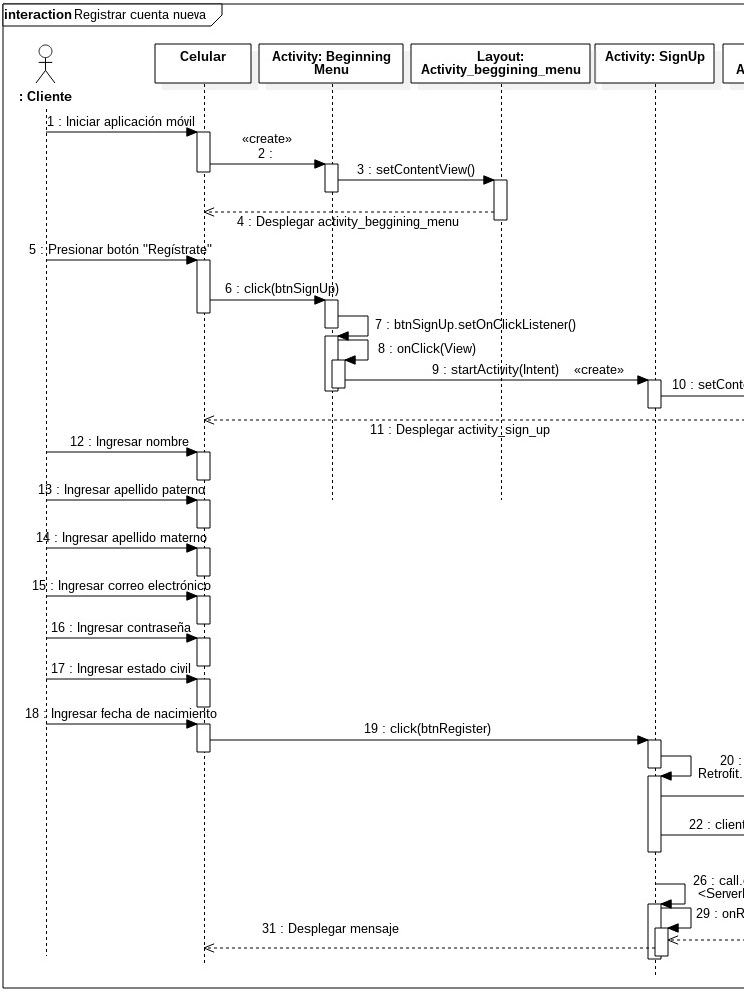
\includegraphics[width=0.9 \textwidth]{imagenes/Diagramas_UserApp/Nuevos_diagramas/CuentaNueva_1}
		\caption{Diagrama de secuencia para registrar cuenta nueva (Parte 1).}
		\label{image:RegistrarCuenta1}
\end{figure}
\FloatBarrier

\FloatBarrier
\begin{figure}[htbp!]
		\centering
			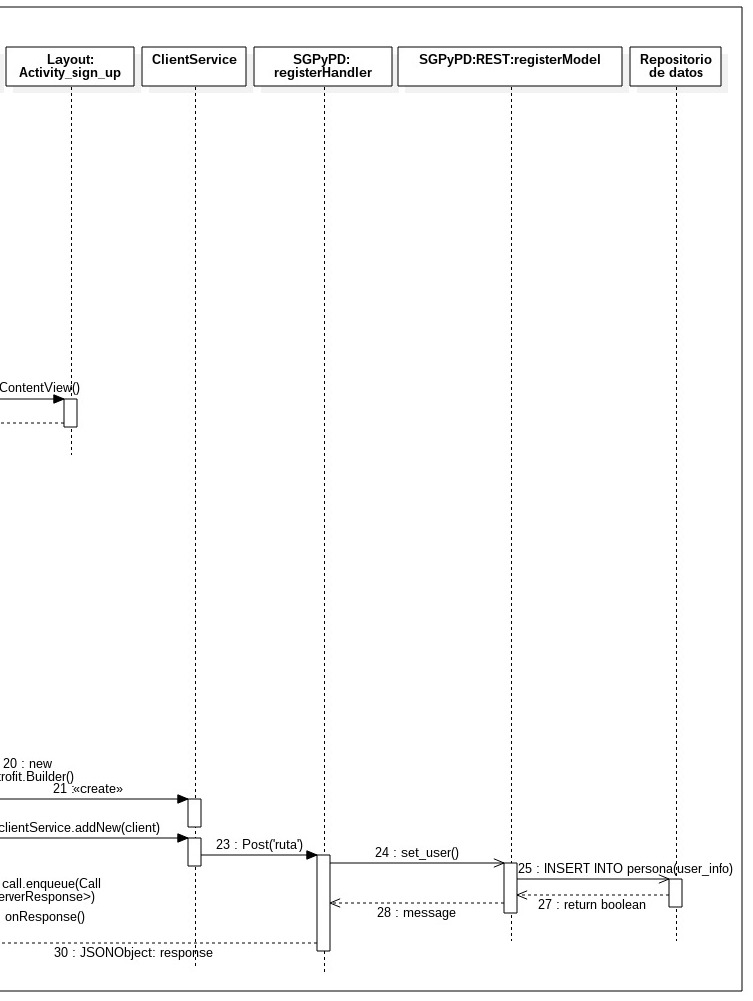
\includegraphics[width=0.9 \textwidth]{imagenes/Diagramas_UserApp/Nuevos_diagramas/CuentaNueva_2}
		\caption{Diagrama de secuencia para registrar cuenta nueva (Parte 2).}
		\label{image:RegistrarCuenta2}
\end{figure}
\FloatBarrier

\title{\textbf{Consultar folletos}}
\\ \par
El diagrama de la figura \ref{image:DSConsultarFolletos1} se dividió en dos secciones para obtener una mejor visualización, dichas secciones corresponden a la figura \ref{image:DSConsultarFolletos2} y \ref{image:DSConsultarFolletos3}. Este diagrama corresponde a la secuencia ``Consultar folletos'' mismo que es desplegado al iniciar sesión en la aplicación y dentro del cual se muestran las promociones y descuentos de tiendas y productos.
\FloatBarrier
\begin{figure}[htbp!]
		\centering
			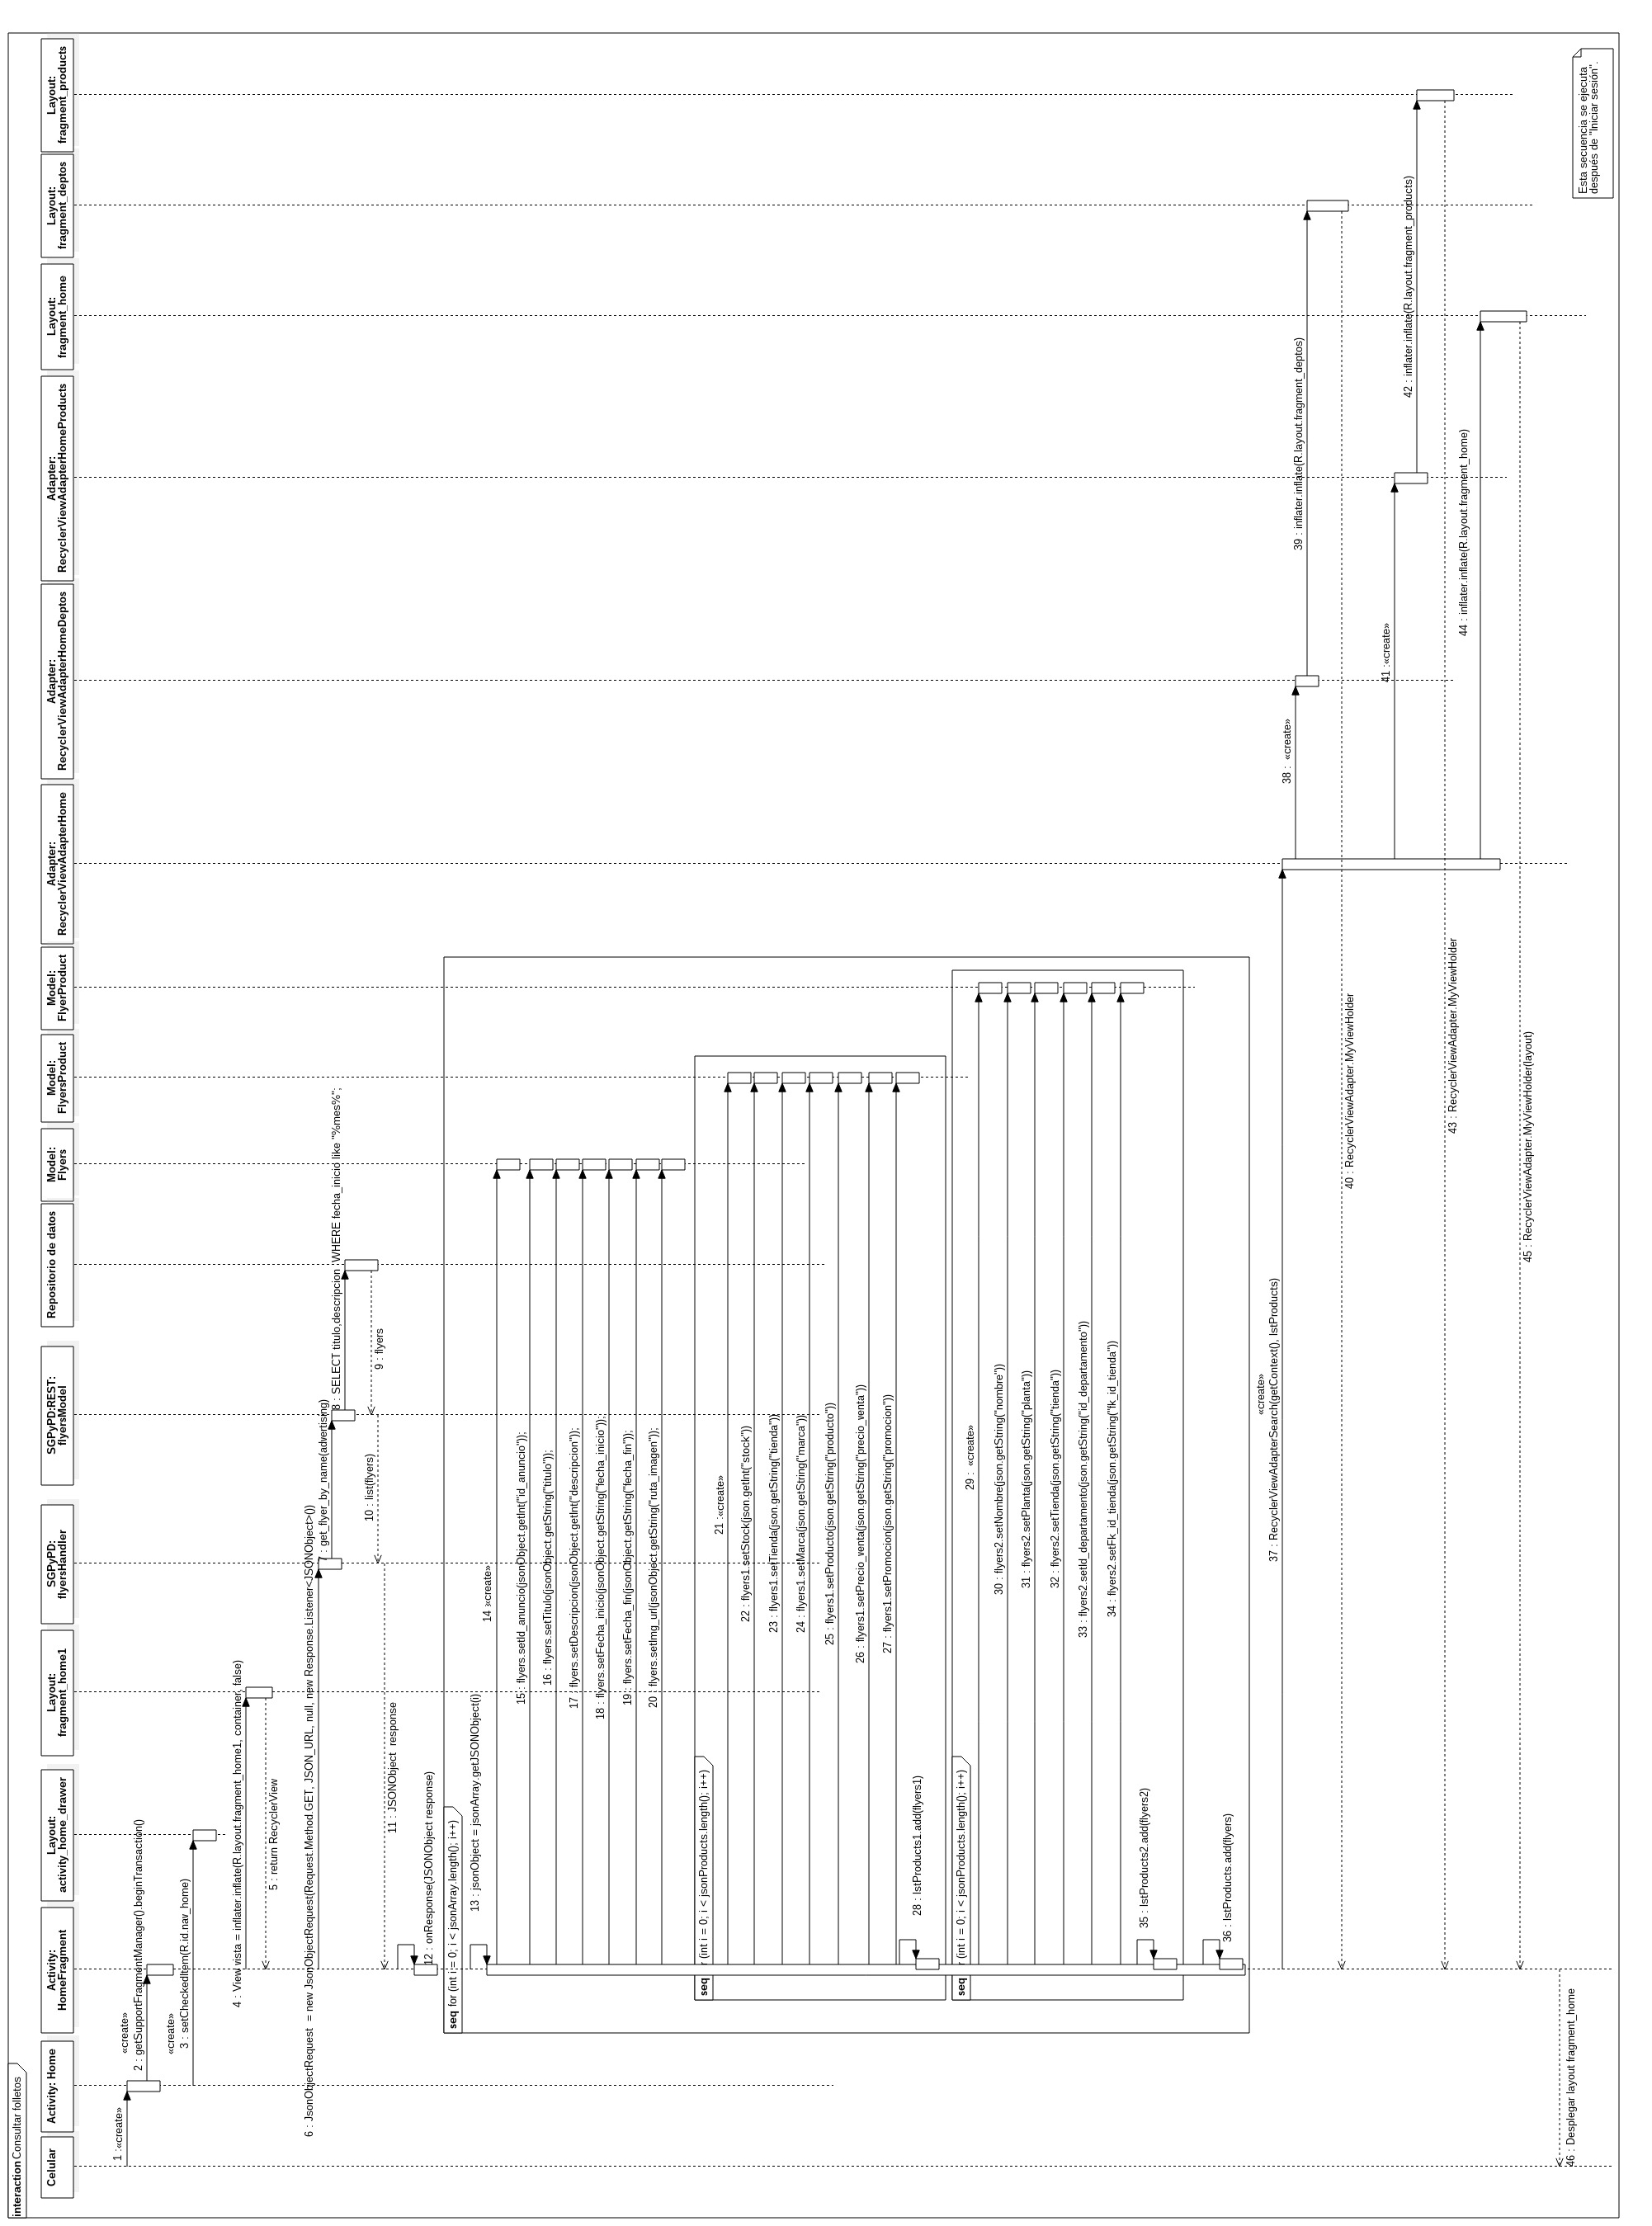
\includegraphics[width=.8 \textwidth]{imagenes/Diagramas_UserApp/Nuevos_diagramas/Horizontal/consultarFolletos}
		\caption{Diagrama de secuencia para consultar folletos (Visualización completa).}
		\label{image:DSConsultarFolletos1}
\end{figure}
\FloatBarrier

\FloatBarrier
\begin{figure}[htbp!]
		\centering
			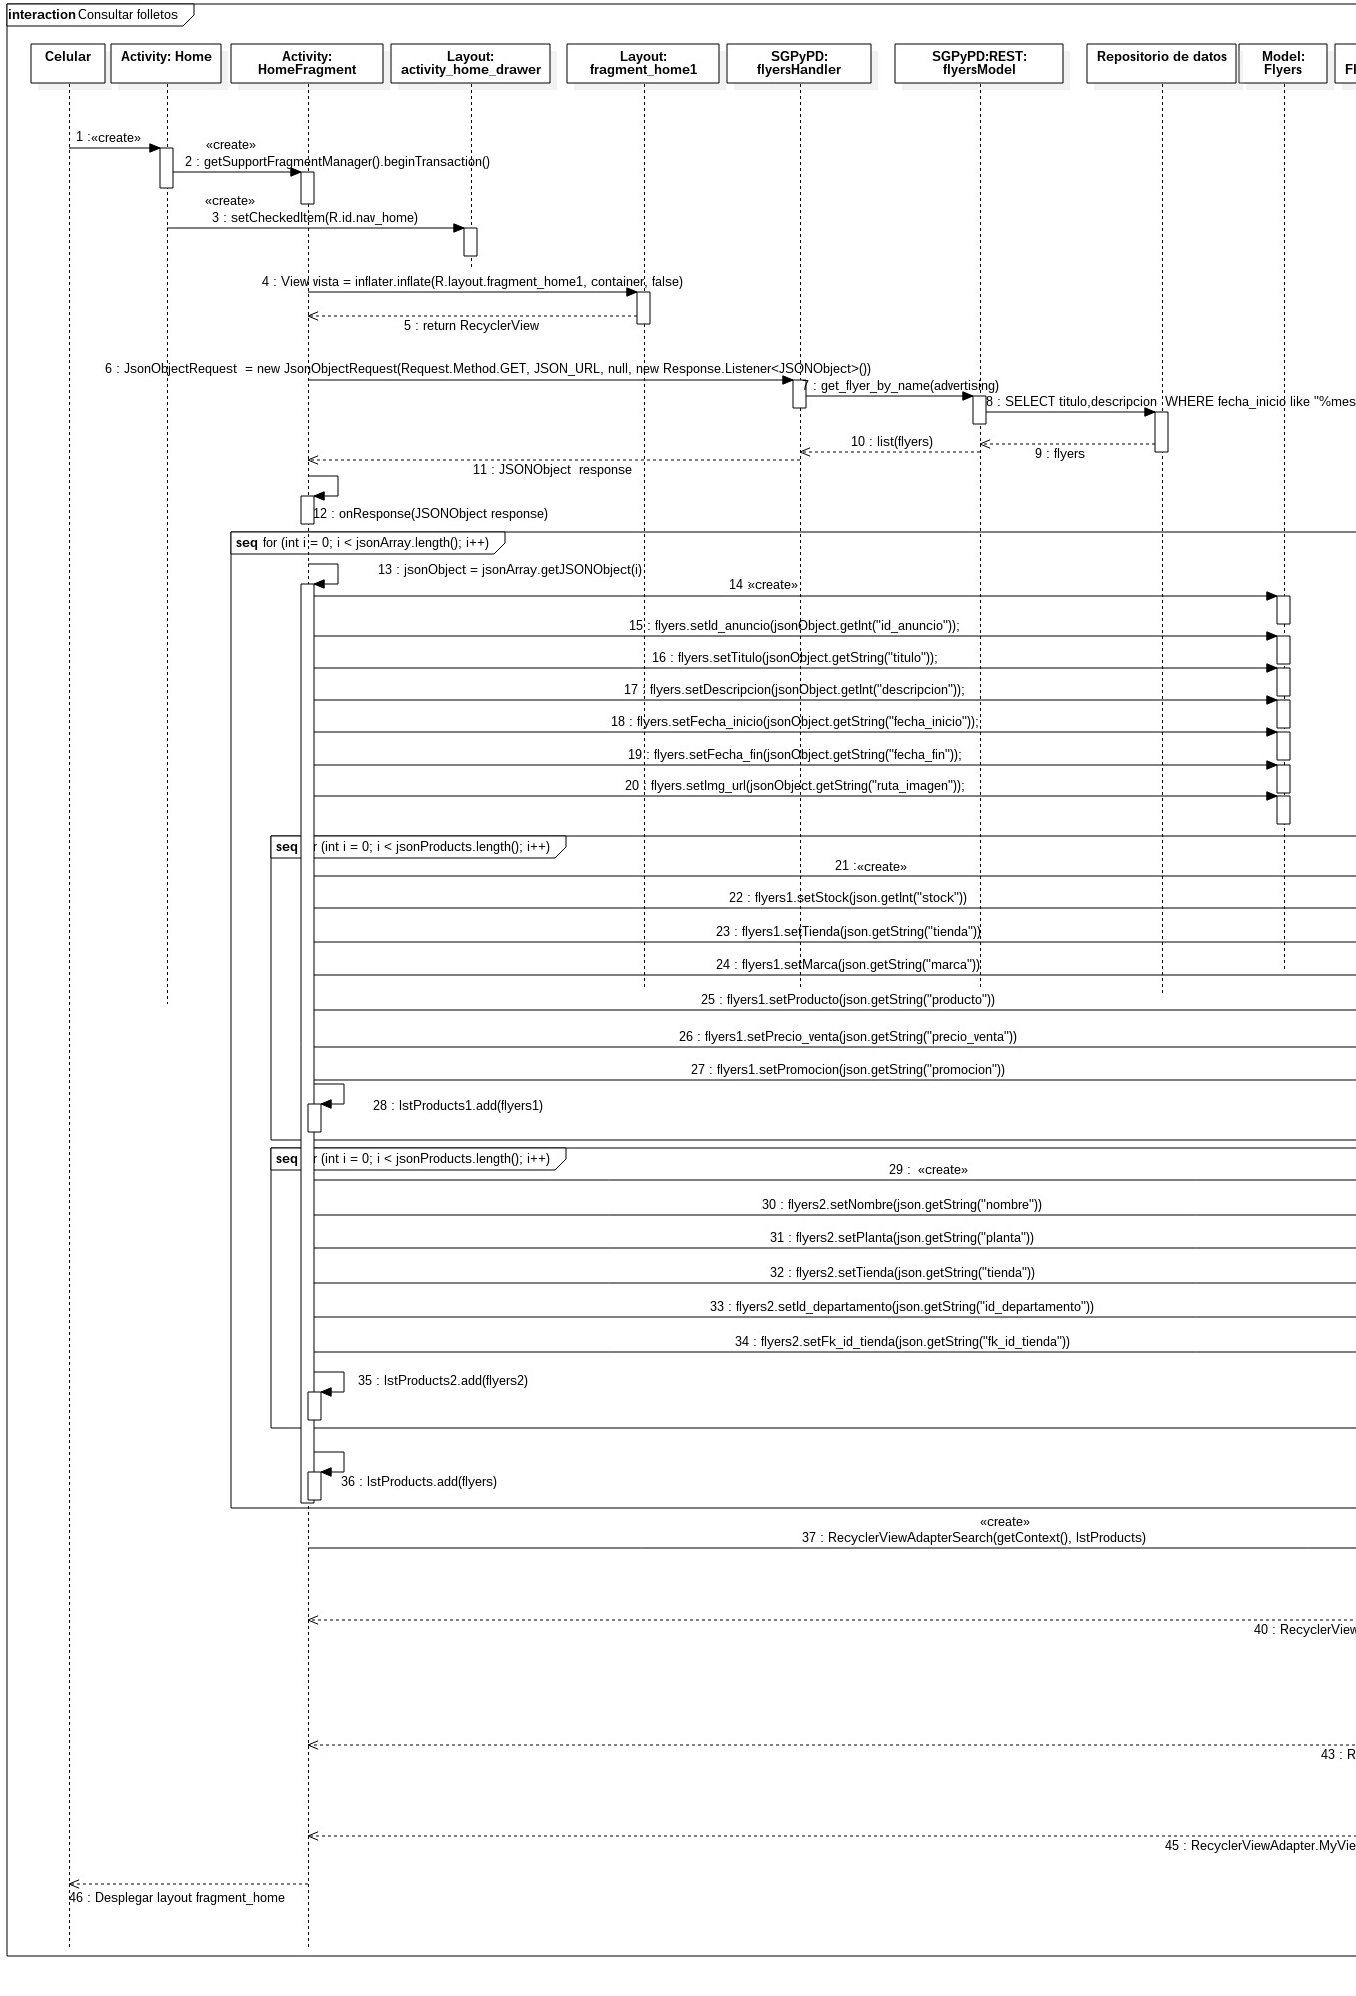
\includegraphics[width=.9 \textwidth]{imagenes/Diagramas_UserApp/Nuevos_diagramas/consultarFolletos1}
		\caption{Diagrama de secuencia para consultar folletos (Parte 1).}
		\label{image:DSConsultarFolletos2}
\end{figure}
\FloatBarrier

\FloatBarrier
\begin{figure}[htbp!]
		\centering
			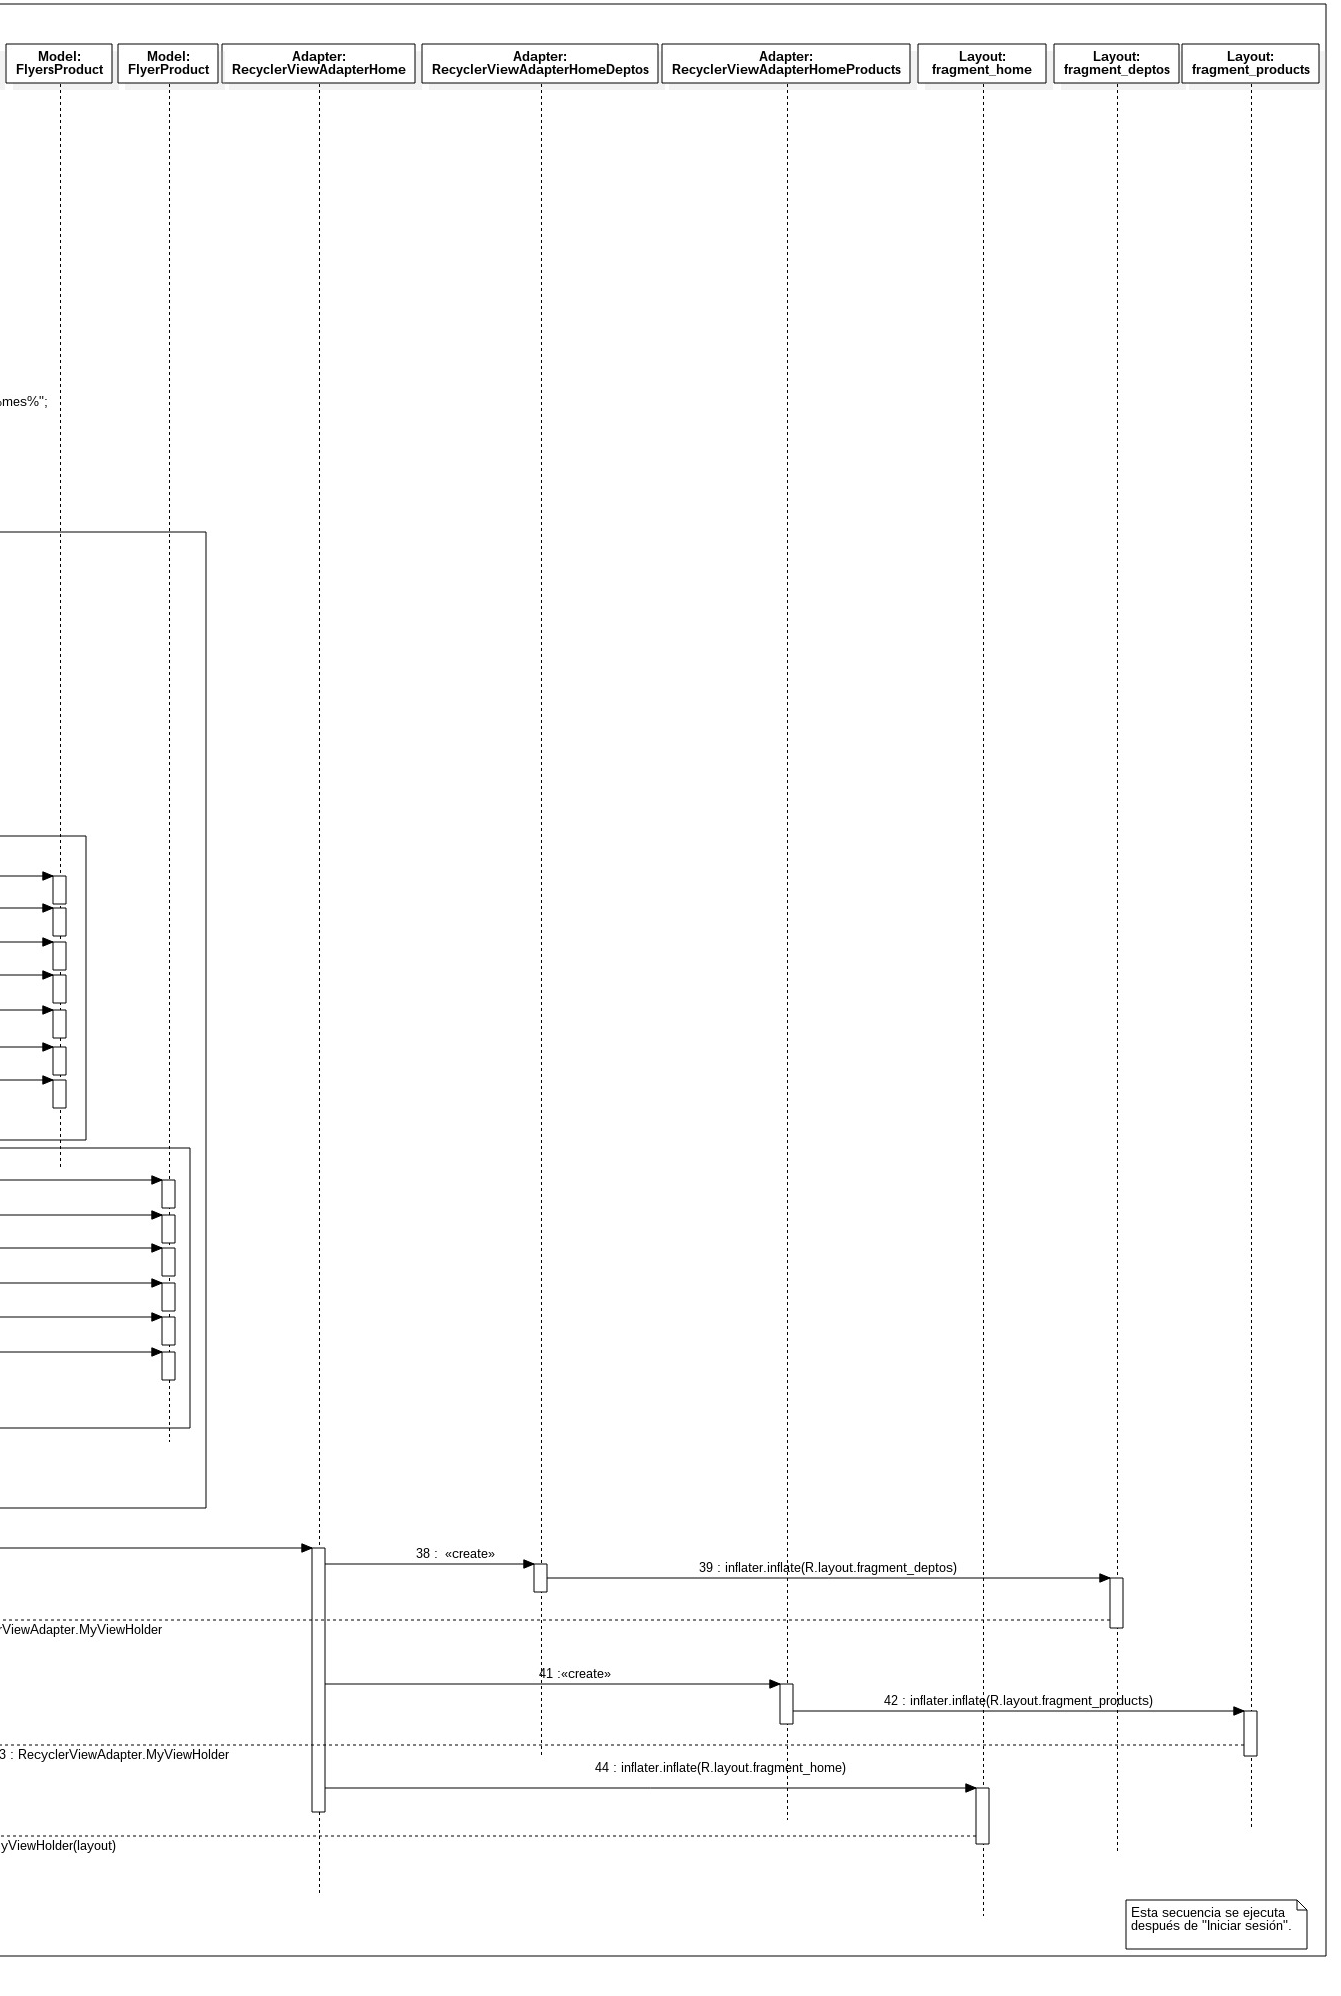
\includegraphics[width=.88 \textwidth]{imagenes/Diagramas_UserApp/Nuevos_diagramas/consultarFolletos2}
		\caption{Diagrama de secuencia para consultar folletos (Parte 2).}
		\label{image:DSConsultarFolletos3}
\end{figure}
\FloatBarrier

\title{\textbf{Visualizar menú de opciones}}
\\ \par
El diagrama de la figura \ref{image:DSvisualizarMenu1}, se dividió en dos secciones para una mejor visualización, estas corresponden a la figura \ref{image:DSVisualizarMenu2} y \ref{image:DSVisualizarMenu3}. Este diagrama pertenece a la secuencia ``Visualizar menú de opciones'', en el cual como su nombre lo dice, se ejecuta el proceso en el que el usuario puede observar las opciones que el menú le proporciona dentro del sistema.
\FloatBarrier
\begin{figure}[htbp!]
		\centering
			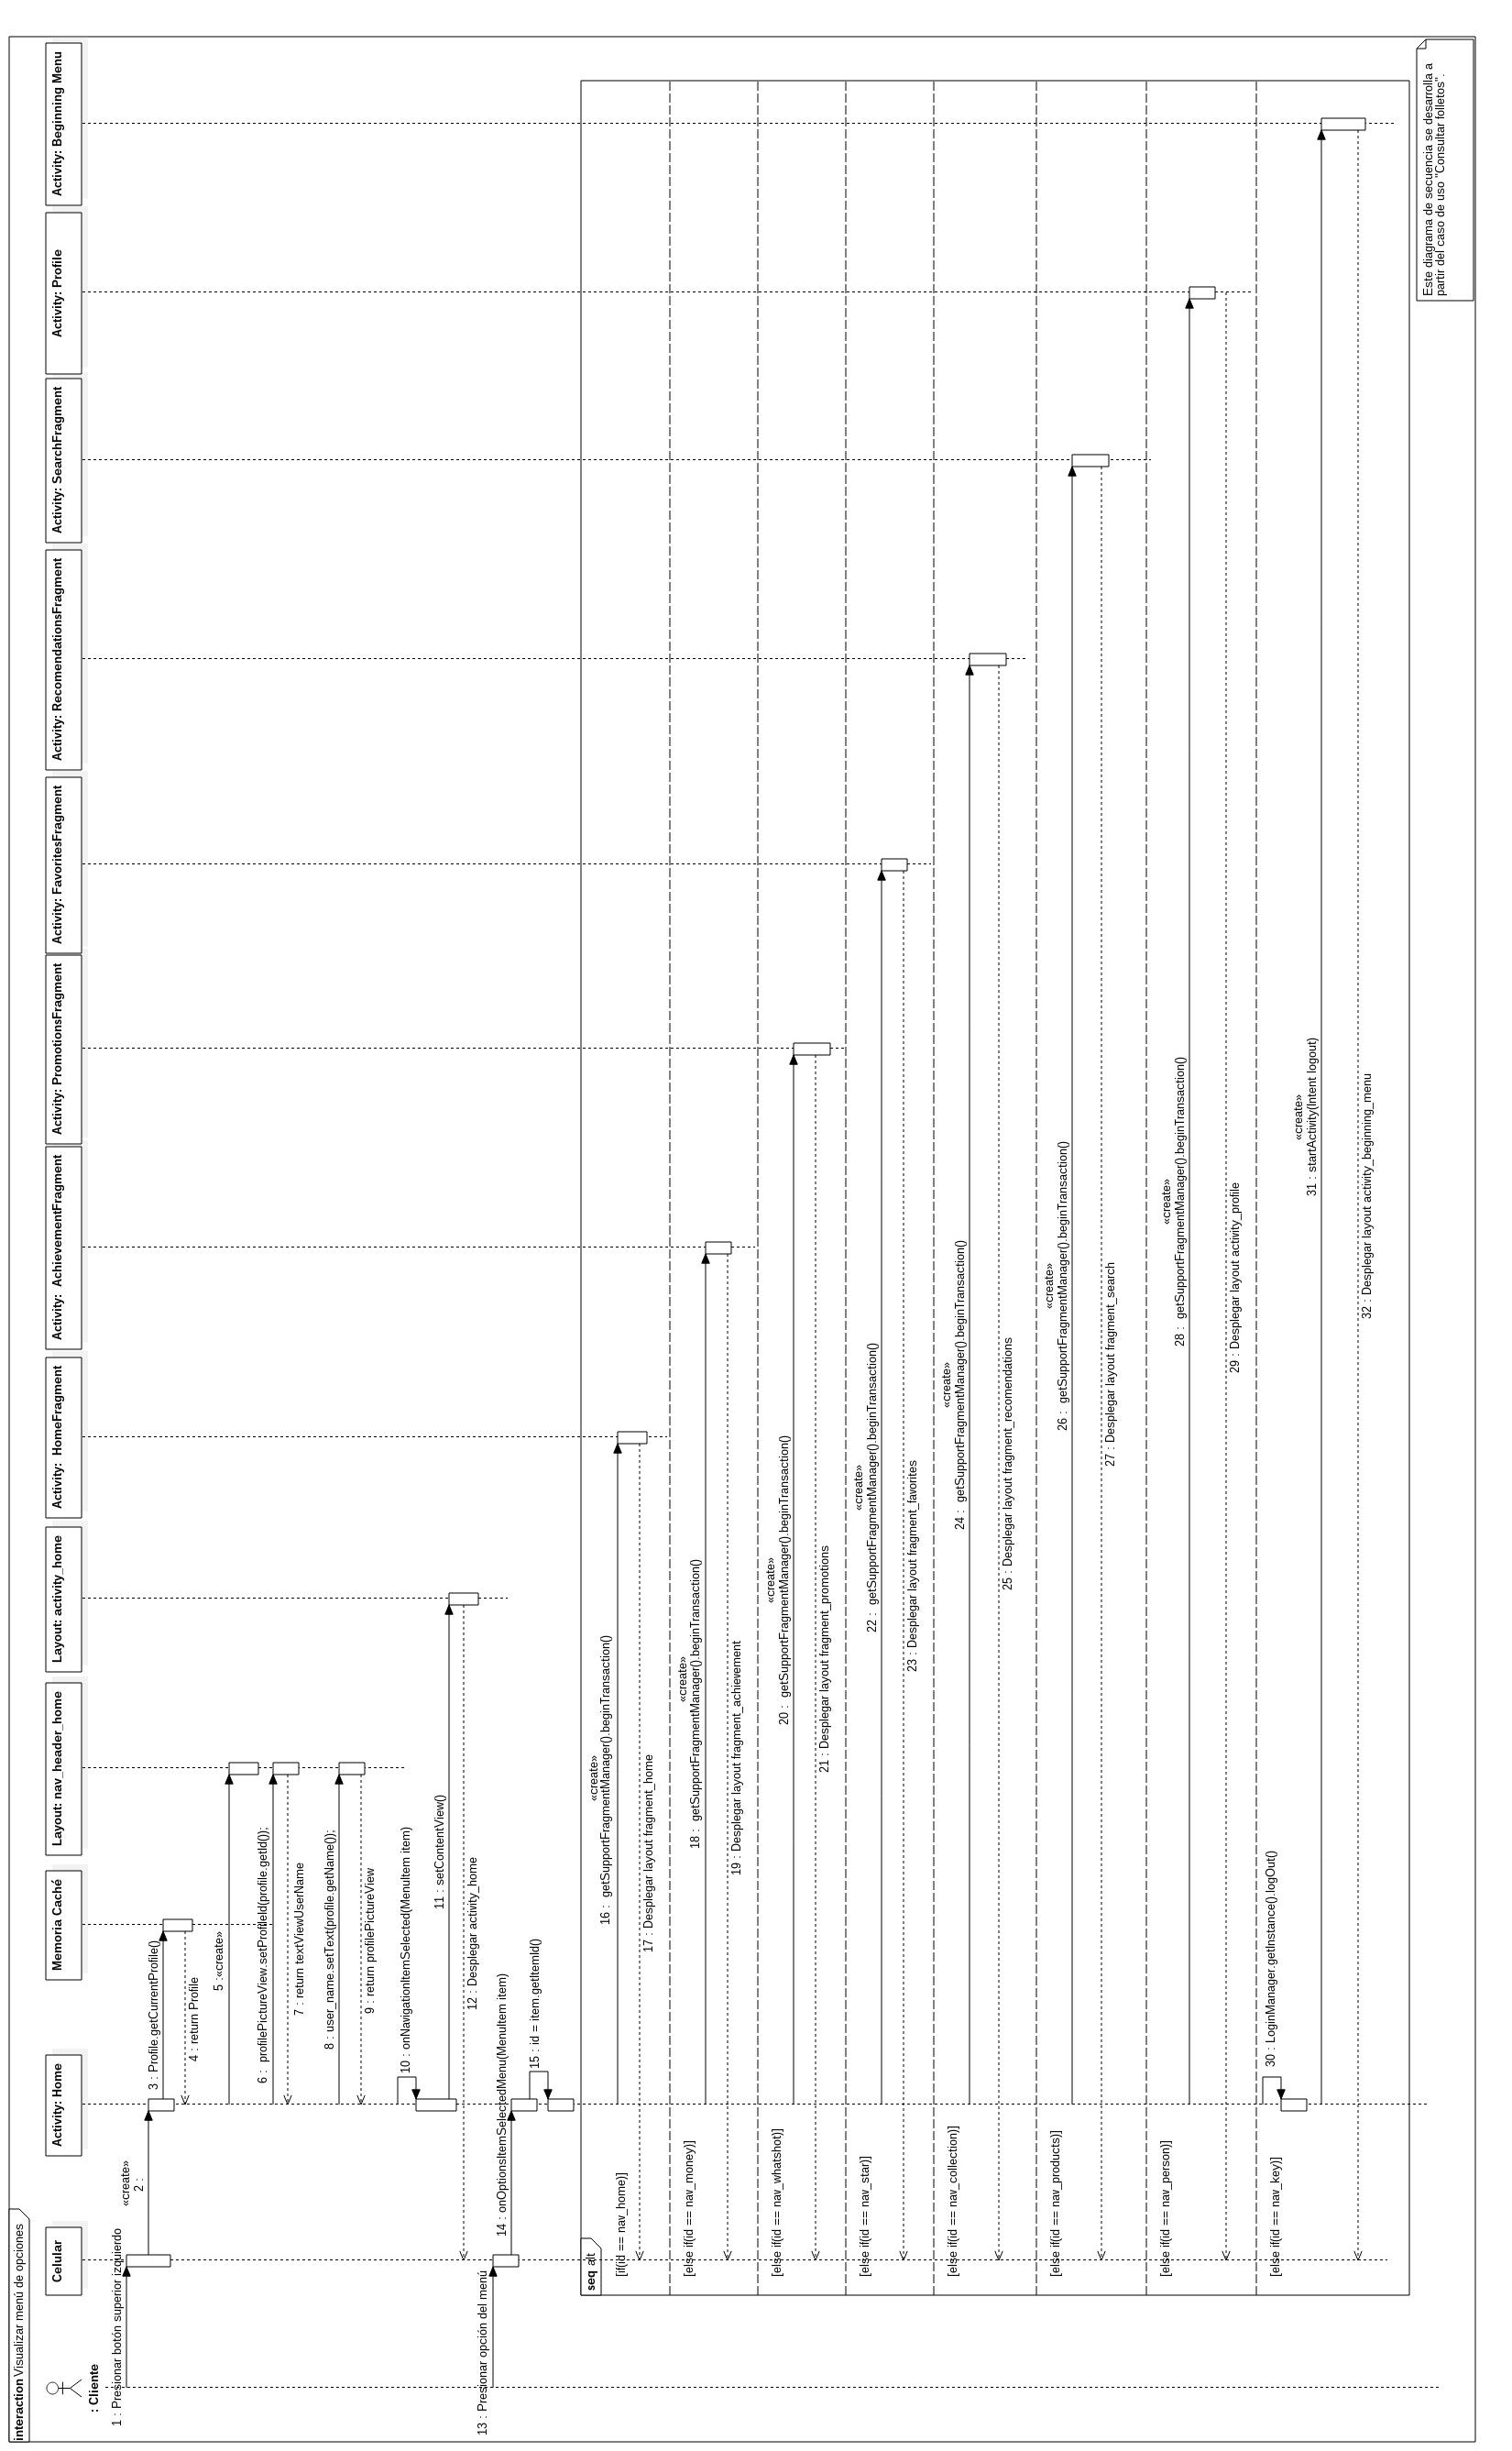
\includegraphics[width=.68 \textwidth]{imagenes/Diagramas_UserApp/Nuevos_diagramas/Horizontal/visualizarMenu}
		\caption{Diagrama de secuencia para visualizar menú de opciones (Visualización completa).}
		\label{image:DSvisualizarMenu1}
\end{figure}
\FloatBarrier

\FloatBarrier
\begin{figure}[htbp!]
		\centering
			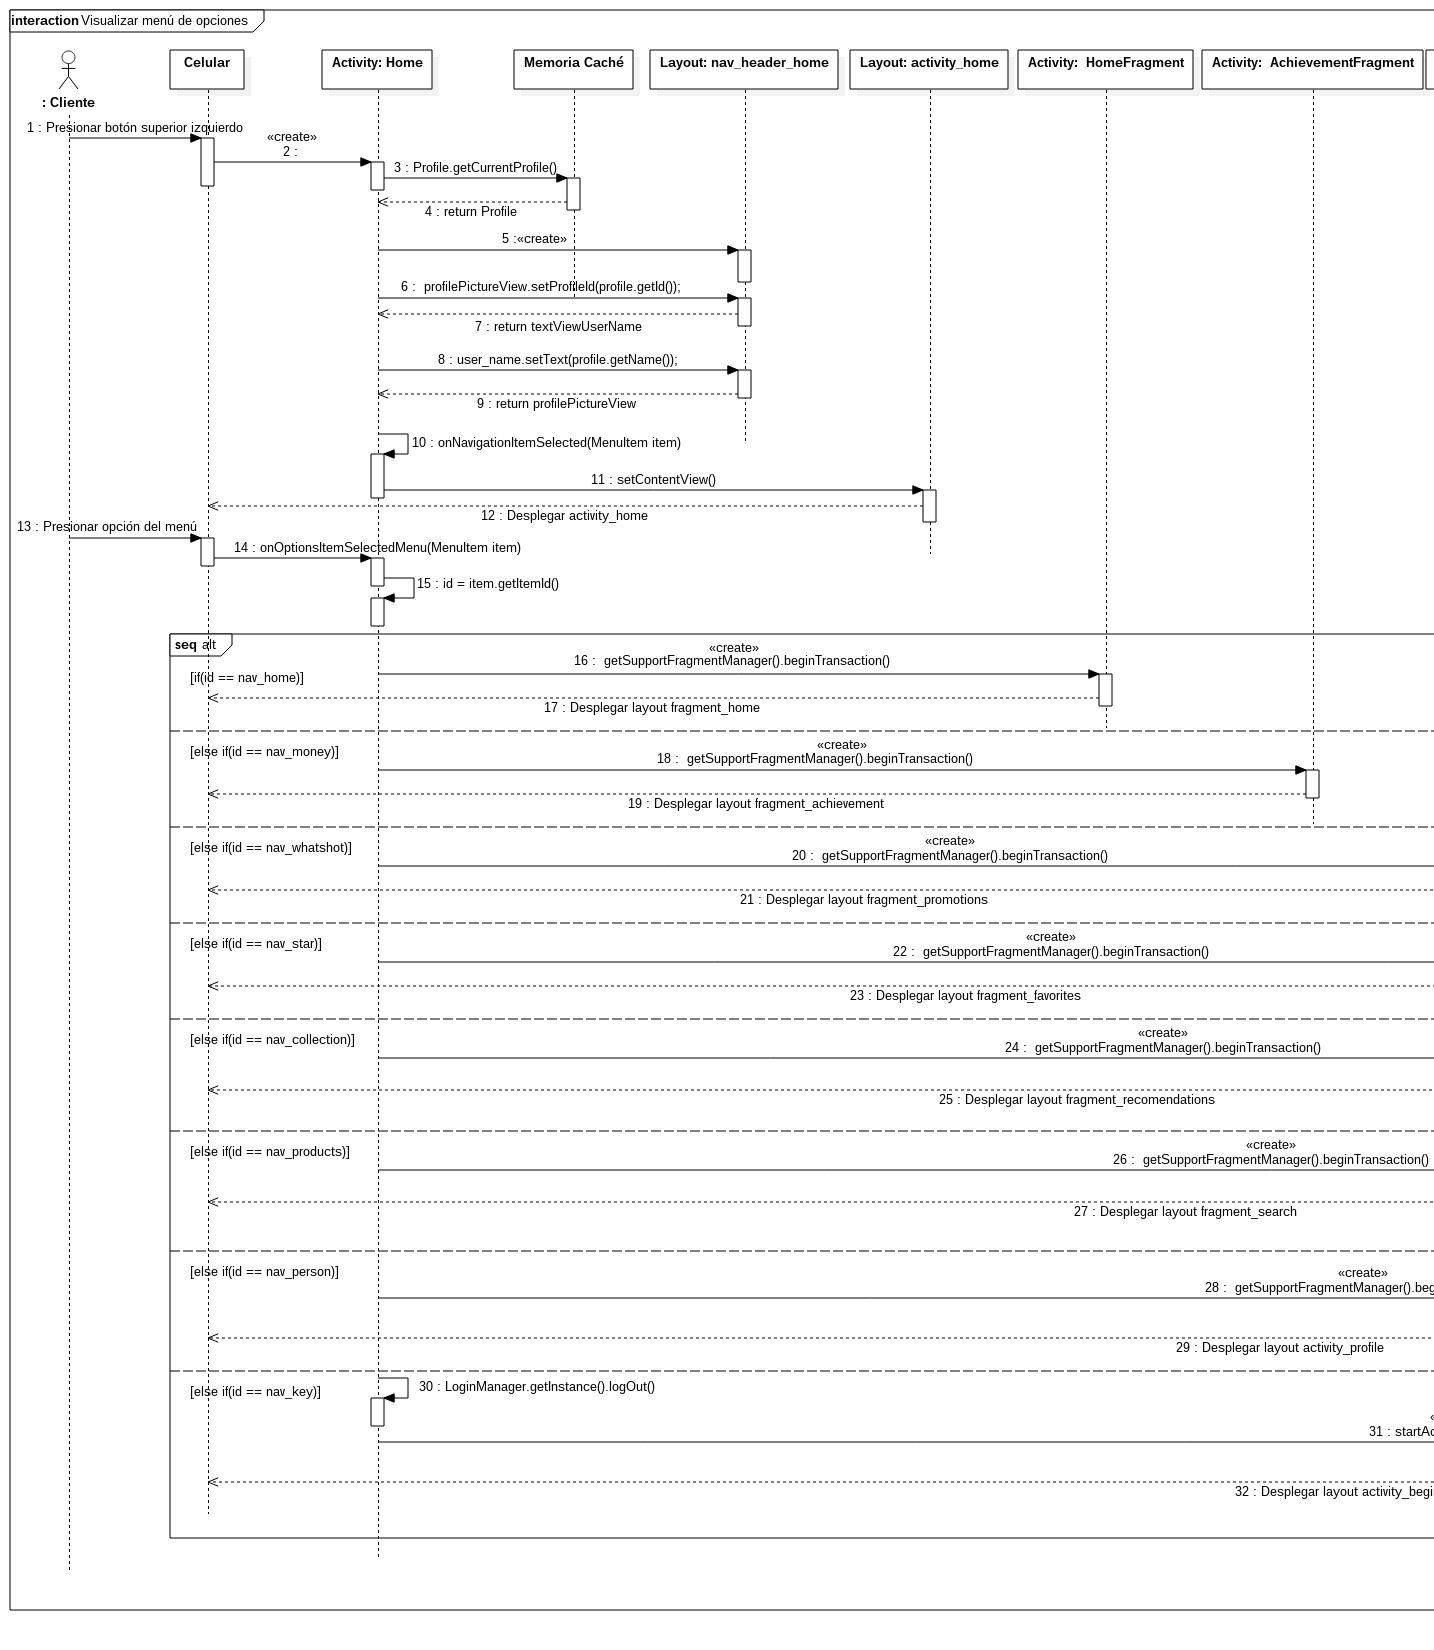
\includegraphics[width=1 \textwidth]{imagenes/Diagramas_UserApp/Nuevos_diagramas/visualizarMenu1}
		\caption{Diagrama de secuencia para visualizar menú de opciones (Parte 1).}
		\label{image:DSVisualizarMenu2}
\end{figure}
\FloatBarrier

\FloatBarrier
\begin{figure}[htbp!]
		\centering
			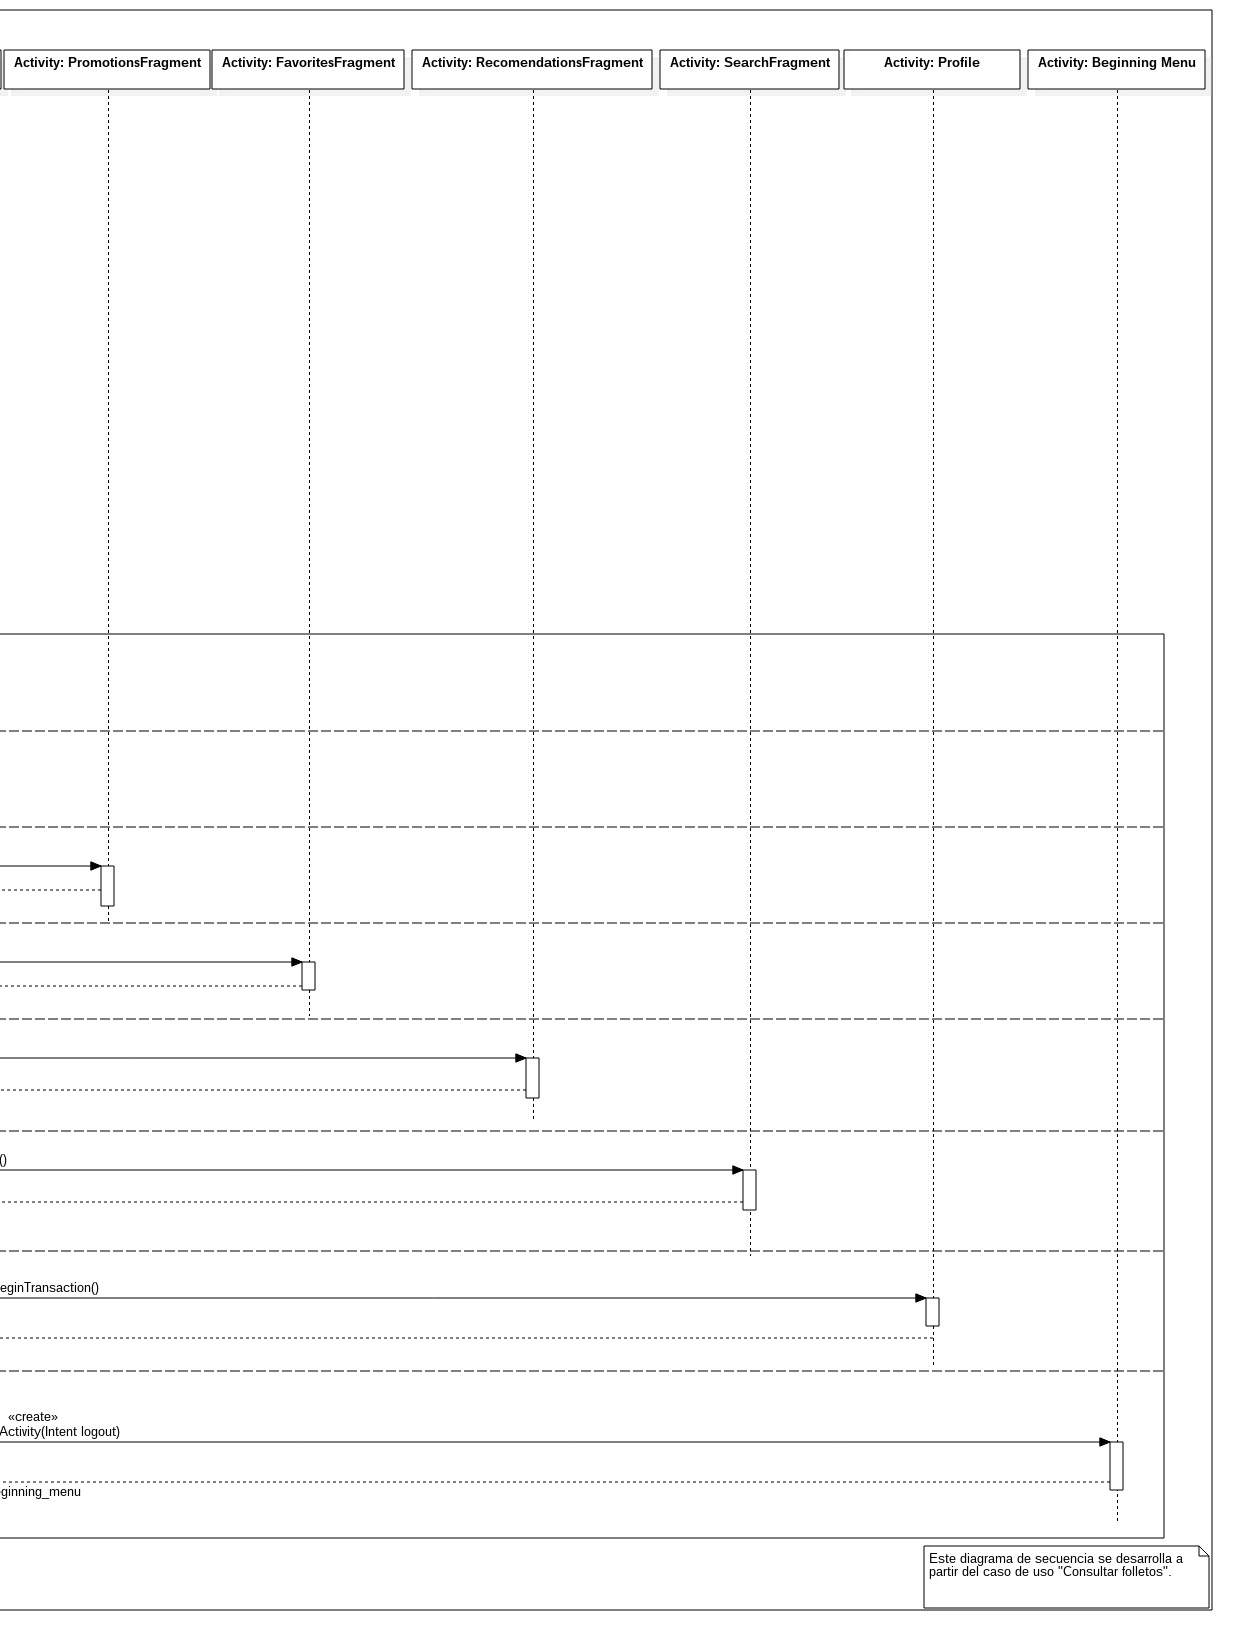
\includegraphics[width=1 \textwidth]{imagenes/Diagramas_UserApp/Nuevos_diagramas/visualizarMenu2}
		\caption{Diagrama de secuencia para visualizar menú de opciones (Parte 2).}
		\label{image:DSVisualizarMenu3}
\end{figure}
\FloatBarrier

\title{\textbf{Consultar logros}}
\\ \par
El diagrama de la figura \ref{image:DSConsultarLogros1} corresponde a la secuencia ``Consultar logros''
, dicha opción se localiza dentro del menú de opciones y despliega la lista de beneficios que obtiene el usuario al obtener un logro en la aplicación. \\ \par
Este se dividió en dos secciones para una mejor visualización, estas corresponden a la figura \ref{image:DSConsultarLogros2} y \ref{image:DSConsultarLogros3}. 
\FloatBarrier
\begin{figure}[htbp!]
		\centering
			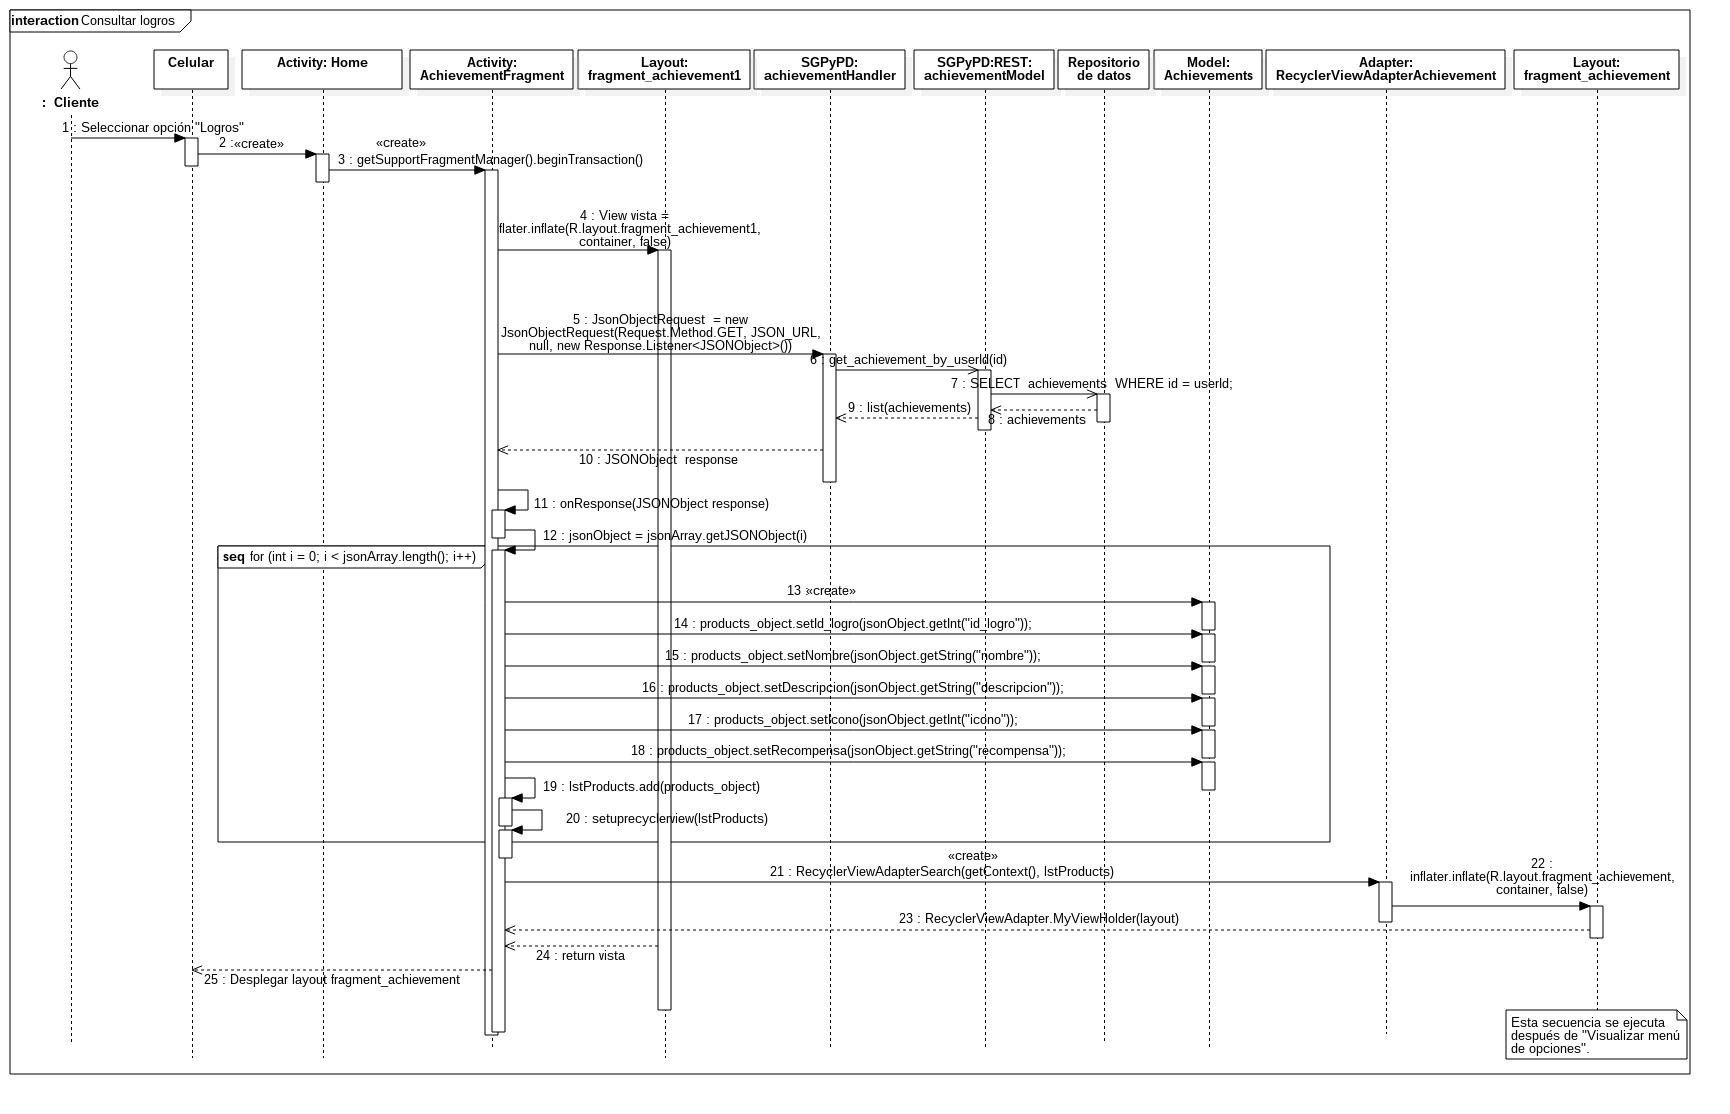
\includegraphics[width=1.1 \textwidth]{imagenes/Diagramas_UserApp/Nuevos_diagramas/Logros}
		\caption{Diagrama de secuencia para consultar logros (Visualización completa).}
		\label{image:DSConsultarLogros1}
\end{figure}
\FloatBarrier

\FloatBarrier
\begin{figure}[htbp!]
		\centering
			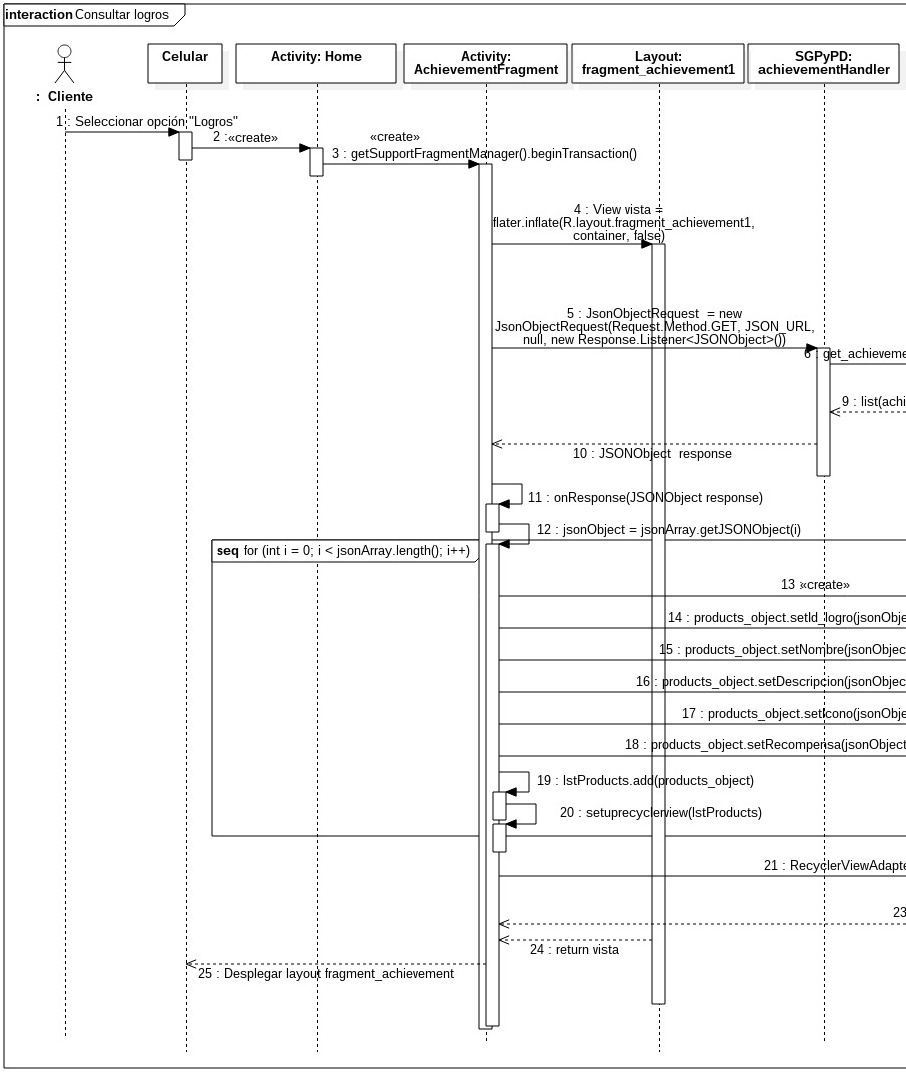
\includegraphics[width=.9 \textwidth]{imagenes/Diagramas_UserApp/Nuevos_diagramas/Logros1}
		\caption{Diagrama de secuencia para consultar logros (Parte 1).}
		\label{image:DSConsultarLogros2}
\end{figure}
\FloatBarrier

\FloatBarrier
\begin{figure}[htbp!]
		\centering
			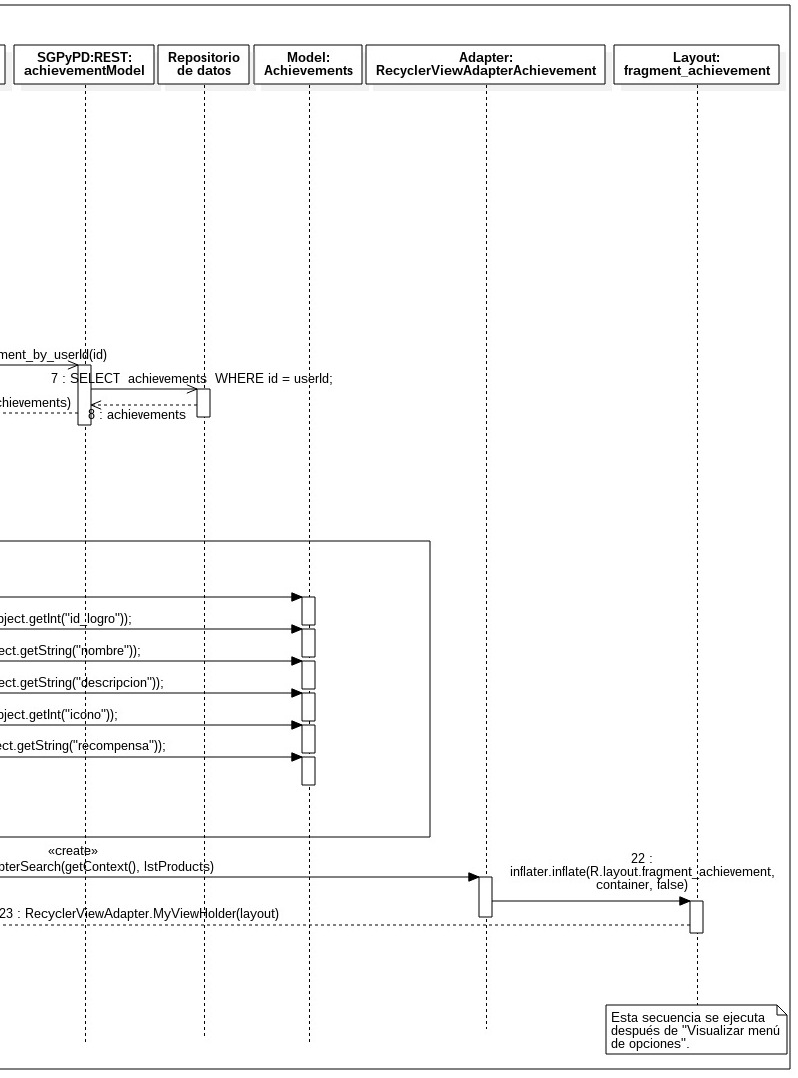
\includegraphics[width=.9 \textwidth]{imagenes/Diagramas_UserApp/Nuevos_diagramas/Logros2}
		\caption{Diagrama de secuencia para consultar logros (Parte 2).}
		\label{image:DSConsultarLogros3}
\end{figure}
\FloatBarrier
\newpage
\title{\textbf{Consultar promociones}}
\\ \par
El diagrama de la figura \ref{image:DSConsultarPromociones1} corresponde a la secuencia ``Consultar promociones'', dicha opción se localiza dentro del menú de opciones y despliega la lista de promociones que hay en las diferentes tiendas debido a una fecha en especial como Navidad o el día de las madres.
\FloatBarrier
\begin{figure}[htbp!]
		\centering
			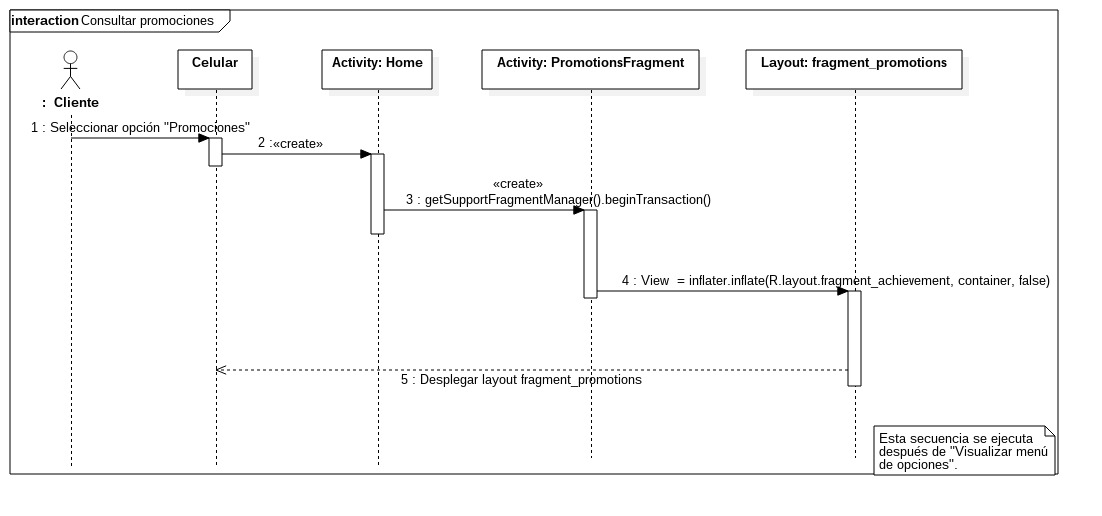
\includegraphics[width=1.1 \textwidth]{imagenes/Diagramas_UserApp/Nuevos_diagramas/Promociones}
		\caption{Diagrama de secuencia para consultar promociones (Visualización completa).}
		\label{image:DSConsultarPromociones1}
\end{figure}
\FloatBarrier

\title{\textbf{Visualizar favoritos}}
\\ \par
El diagrama de la figura \ref{image:favs1}, se dividió en dos secciones para una mejor visualización, estas corresponden a la figura \ref{image:favs2} y \ref{image:favs3}. Este diagrama pertenece a la secuencia ``Visualizar favoritos'', en el cual como su nombre lo dice, permite al usuario observar los productos que ha seleccionado anteriormente como favorito.
\FloatBarrier
\begin{figure}[htbp!]
		\centering
			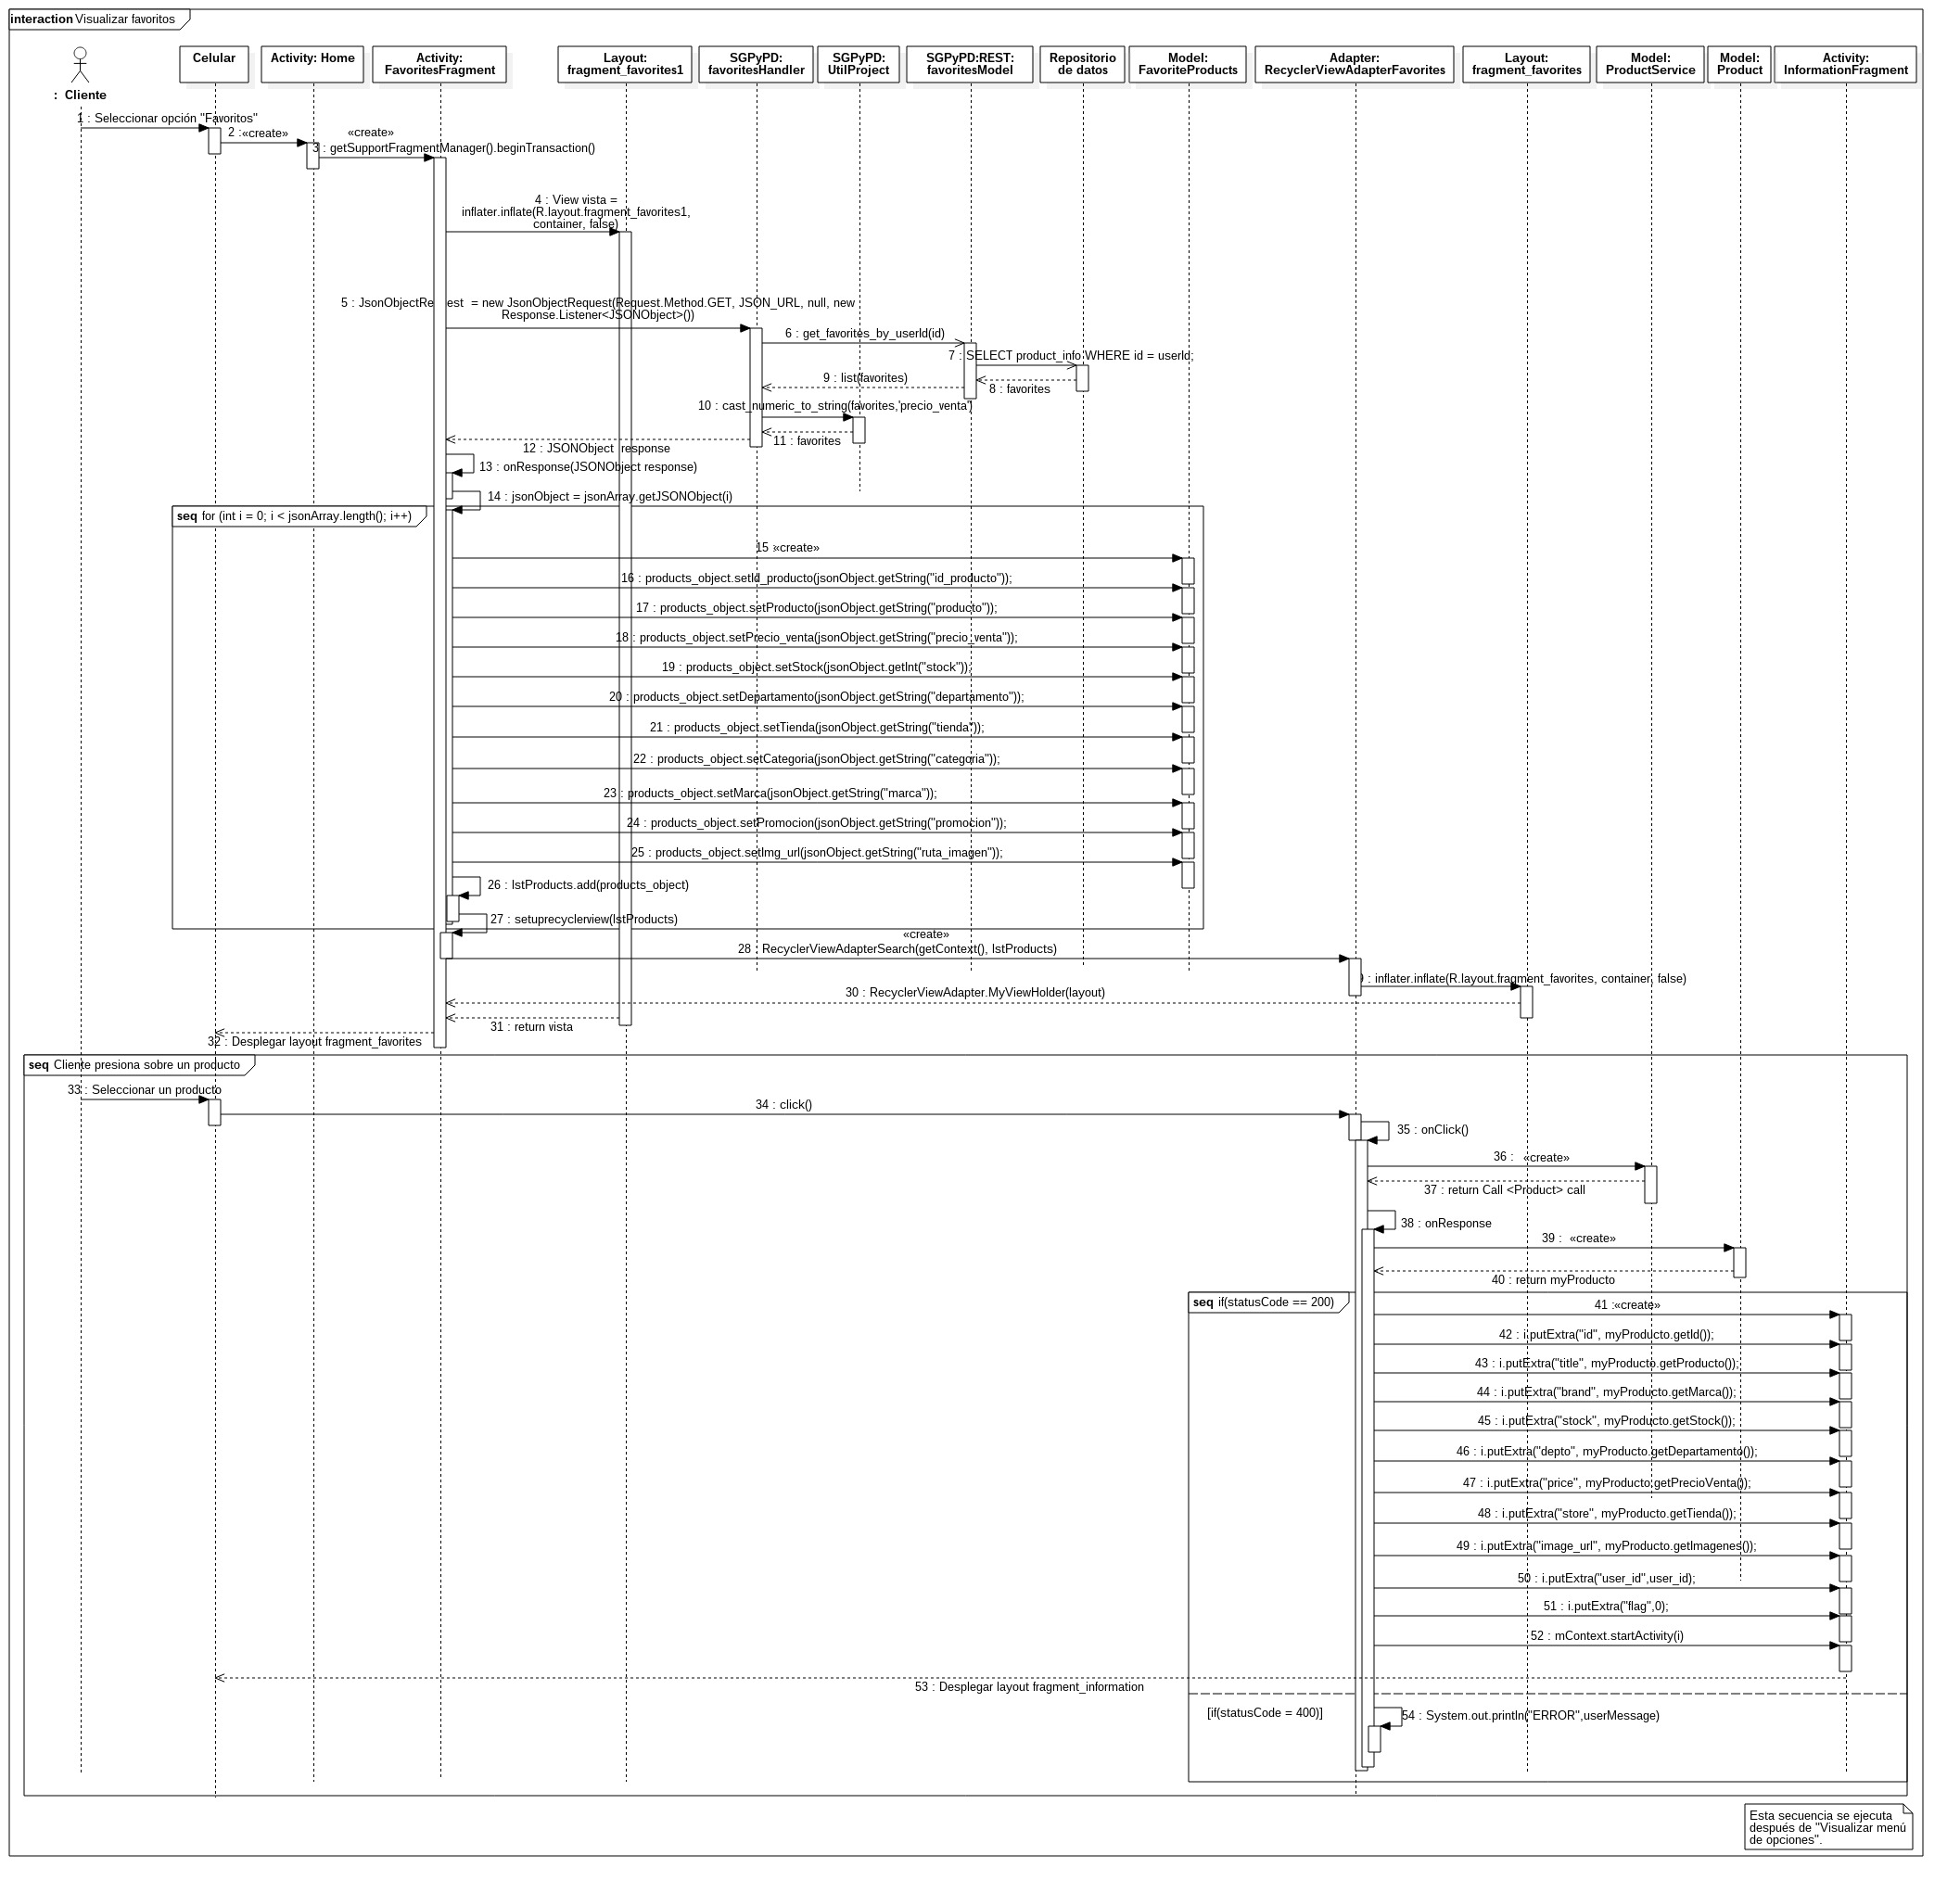
\includegraphics[width=1.1 \textwidth]{imagenes/Diagramas_UserApp/Nuevos_diagramas/Favoritos}
		\caption{Diagrama de secuencia para visualizar favoritos (Visualización completa).}
		\label{image:favs1}
\end{figure}
\FloatBarrier

\FloatBarrier
\begin{figure}[htbp!]
		\centering
			\includegraphics[width=.72 \textwidth]{imagenes/Diagramas_UserApp/Nuevos_diagramas/Favoritos1}
		\caption{Diagrama de secuencia para visualizar favoritos (Parte 1).}
		\label{image:favs2}
\end{figure}
\FloatBarrier

\FloatBarrier
\begin{figure}[htbp!]
		\centering
			\includegraphics[width=.65 \textwidth]{imagenes/Diagramas_UserApp/Nuevos_diagramas/Favoritos2}
		\caption{Diagrama de secuencia para visualizar favoritos (Parte 2).}
		\label{image:favs3}
\end{figure}
\FloatBarrier

\title{\textbf{Añadir/Eliminar producto de favoritos}}
\\ \par
El diagrama de la figura \ref{image:addDelFav} se muestran las secuencias ``Añadir producto a favoritos'' y ``Eliminar producto de favoritos''. Es importante recalcar que se observan dichas secuencias juntas debido a que ambas hacen uso de una misma clase para realizar su funcionamiento, únicamente difiere en ellas la visibilidad de uno u otro botón, mismo que igual se plasma en dicho diagrama.
\FloatBarrier
\begin{figure}[htbp!]
		\centering
			\includegraphics[width=.96 \textwidth]{imagenes/Diagramas_UserApp/Nuevos_diagramas/anadir_eliminarFav}
		\caption{Diagrama de secuencia para añadir o eliminar productos a favoritos (Visualización completa).}
		\label{image:addDelFav}
\end{figure}
\FloatBarrier

\title{\textbf{Consultar recomendaciones}}
\\ \par
El diagrama de la figura \ref{image:rec1}, se dividió en dos secciones para una mejor visualización, estas corresponden a la figura \ref{image:rec2} y \ref{image:rec3}. Este diagrama pertenece a la secuencia ``Consultar recomendaciones''. En esta sección aún no se ha implementado la funcionalidad de recibir los productos recomendados particularmente para un cliente, sin embargo se observa la secuencia del como se desplegarían los productos obtenidos.
\FloatBarrier
\begin{figure}[htbp!]
		\centering
			\includegraphics[width=1.1 \textwidth]{imagenes/Diagramas_UserApp/Nuevos_diagramas/Recomendaciones}
		\caption{Diagrama de secuencia para consultar recomendaciones (Visualización completa).}
		\label{image:rec1}
\end{figure}
\FloatBarrier

\FloatBarrier
\begin{figure}[htbp!]
		\centering
			\includegraphics[width=.68 \textwidth]{imagenes/Diagramas_UserApp/Nuevos_diagramas/Recomendaciones1}
		\caption{Diagrama de secuencia para consultar recomendaciones (Parte 1).}
		\label{image:rec2}
\end{figure}
\FloatBarrier

\FloatBarrier
\begin{figure}[htbp!]
		\centering
			\includegraphics[width=.62 \textwidth]{imagenes/Diagramas_UserApp/Nuevos_diagramas/Recomendaciones2}
		\caption{Diagrama de secuencia para consultar recomendaciones (Parte 2).}
		\label{image:rec3}
\end{figure}
\FloatBarrier

\title{\textbf{Buscar productos}}
\\ \par
El diagrama de la figura \ref{image:busca1}, se dividió en dos secciones para una mejor visualización, estas corresponden a la figura \ref{image:busca2} y \ref{image:busca3}. Este diagrama pertenece a la secuencia ``Buscar productos ''. Esta sección permite al usuario buscar por nombre productos que resulten ser de su interés.

\FloatBarrier
\begin{figure}[htbp!]
		\centering
			\includegraphics[width=1.1 \textwidth]{imagenes/Diagramas_UserApp/Nuevos_diagramas/buscarPoductos}
		\caption{Diagrama de secuencia para buscar productos (Visualización completa).}
		\label{image:busca1}
\end{figure}
\FloatBarrier

\FloatBarrier
\begin{figure}[htbp!]
		\centering
			\includegraphics[width=.65 \textwidth]{imagenes/Diagramas_UserApp/Nuevos_diagramas/buscarPoductos1}
		\caption{Diagrama de secuencia para buscar productos (Parte 1).}
		\label{image:busca2}
\end{figure}
\FloatBarrier

\FloatBarrier
\begin{figure}[htbp!]
		\centering
			\includegraphics[width=.6 \textwidth]{imagenes/Diagramas_UserApp/Nuevos_diagramas/buscarPoductos2}
		\caption{Diagrama de secuencia para buscar productos (Parte 2).}
		\label{image:busca3}
\end{figure}
\FloatBarrier

\title{\textbf{Actualizar datos personales y consultar nivel}}
\\ \par
El diagrama de la figura \ref{image:consulta1}, se dividió en dos secciones para una mejor visualización, estas corresponden a la figura \ref{image:consulta2} y \ref{image:consulta3}. Este diagrama pertenece a la secuencia ``Consultar datos personales ''. 
\textit{Nota: Este diagrama contiene la secuencia para el caso de uso `` CUAIDP9: Actualizar datos personales'' y `` CUAIDP9.1: Consultar nivel'' debido a que al solicitar los datos de un usuario al servidor, igualmente se recibe el nivel en el que el cliente se encuentra en ese momento. Sin embargo, es importante mencionar que al utilizar una clase en común con otros casos de uso, se ven en este plasmado solamente la funcionalidad básica del `` CUAIDP9.2: Actualizar gustos genéricos'', `` CUAIDP9.3: Consultar beneficios'' y del `` CUAIDP9.4: Actualizar permisos''.}
\FloatBarrier
\begin{figure}[htbp!]
		\centering
			\includegraphics[width=.67 \textwidth]{imagenes/Diagramas_UserApp/Nuevos_diagramas/Horizontal/VerPerfil}
		\caption{Diagrama de secuencia para consultar datos personales (Visualización completa).}
		\label{image:consulta1}
\end{figure}
\FloatBarrier

\FloatBarrier
\begin{figure}[htbp!]
		\centering
			\includegraphics[width=1 \textwidth]{imagenes/Diagramas_UserApp/Nuevos_diagramas/VerPerfil_1}
		\caption{Diagrama de secuencia para consultar datos personales (Parte 1).}
		\label{image:consulta2}
\end{figure}
\FloatBarrier

\FloatBarrier
\begin{figure}[htbp!]
		\centering
			\includegraphics[width=.95 \textwidth]{imagenes/Diagramas_UserApp/Nuevos_diagramas/VerPerfil_2}
		\caption{Diagrama de secuencia para consultar datos personales (Parte 2).}
		\label{image:consulta3}
\end{figure}
\FloatBarrier

\title{\textbf{Actualizar gustos genéricos}}
\\ \par
El diagrama de la figura \ref{image:gustos}, se dividió en dos secciones para una mejor visualización, estas corresponden a la figura \ref{image:gustos2} y \ref{image:gustos3}. Este diagrama pertenece a la secuencia ``Actualizar gustos genéricos ''. Esta sección permite al usuario marcar las categorías que se asemejen más a sus gustos.\\
\textit{Nota: Este diagrama contiene la secuencia para el caso de uso `` CUAIDP9.2: Actualizar gustos genéricos'', sin embargo, al utilizar una clase en común con otros casos de uso, se ven en este plasmado solamente la funcionalidad básica del `` CUAIDP9: Actualizar datos personales'', `` CUAIDP9.3: Consultar beneficios'' y del `` CUAIDP9.4: Actualizar permisos''.}
\FloatBarrier
\begin{figure}[htbp!]
		\centering
			\includegraphics[width=1.1 \textwidth]{imagenes/Diagramas_UserApp/Nuevos_diagramas/gustosGenericos}
		\caption{Diagrama de secuencia para actualizar gustos genéricos (Visualización completa).}
		\label{image:gustos}
\end{figure}
\FloatBarrier

\FloatBarrier
\begin{figure}[htbp!]
		\centering
			\includegraphics[width=1 \textwidth]{imagenes/Diagramas_UserApp/Nuevos_diagramas/VerPerfil_1}
		\caption{Diagrama de secuencia para actualizar gustos genéricos (Parte 1).}
		\label{image:gustos2}
\end{figure}
\FloatBarrier

\FloatBarrier
\begin{figure}[htbp!]
		\centering
			\includegraphics[width=.95 \textwidth]{imagenes/Diagramas_UserApp/Nuevos_diagramas/VerPerfil_2}
		\caption{Diagrama de secuencia para actualizar gustos genéricos (Parte 2).}
		\label{image:gustos3}
\end{figure}
\FloatBarrier

\title{\textbf{Consultar beneficios}}
\\ \par
El diagrama de la figura \ref{image:beneficios}, se dividió en dos secciones para una mejor visualización, estas corresponden a la figura \ref{image:beneficios2} y \ref{image:beneficios3}. Este diagrama pertenece a la secuencia ``Consultar beneficios''. Esta sección permite al usuario consultar los beneficios que ha adquirido con respecto al nivel en el que se encuentra actualmente.\\
\textit{Nota: Este diagrama contiene la secuencia para el caso de uso `` CUAIDP9.3: Consultar beneficios'' , sin embargo, al utilizar una clase en común con otros casos de uso, se ven en este plasmado solamente la funcionalidad básica del `` CUAIDP9: Actualizar datos personales'',  `` CUAIDP9.2: Actualizar gustos genéricos'' y del `` CUAIDP9.4: Actualizar permisos''.}
\FloatBarrier
\begin{figure}[htbp!]
		\centering
			\includegraphics[width=.5 \textwidth]{imagenes/Diagramas_UserApp/Nuevos_diagramas/Horizontal/beneficios}
		\caption{Diagrama de secuencia para consultar beneficios (Visualización completa).}
		\label{image:beneficios}
\end{figure}
\FloatBarrier

\FloatBarrier
\begin{figure}[htbp!]
		\centering
			\includegraphics[width=1 \textwidth]{imagenes/Diagramas_UserApp/Nuevos_diagramas/beneficios1}
		\caption{Diagrama de secuencia para consultar beneficios (Parte 1).}
		\label{image:beneficios2}
\end{figure}
\FloatBarrier

\FloatBarrier
\begin{figure}[htbp!]
		\centering
			\includegraphics[width=.9 \textwidth]{imagenes/Diagramas_UserApp/Nuevos_diagramas/beneficios2}
		\caption{Diagrama de secuencia para consultar beneficios (Parte 2).}
		\label{image:beneficios3}
\end{figure}
\FloatBarrier

\title{\textbf{Actualizar permisos}}
\\ \par
El diagrama de la figura \ref{image:permisos}, se dividió en dos secciones para una mejor visualización, estas corresponden a la figura \ref{image:permisos2} y \ref{image:permisos3}. Este diagrama pertenece a la secuencia ``Actualizar permisos''. Esta sección permite al usuario marcar los permisos a los que dará acceso al vendedor para poder ofrecer productos más acorde con sus preferencias.\\
\textit{Nota: Este diagrama contiene la secuencia para el caso de uso `` CUAIDP9.4: Actualizar permisos'', sin embargo, al utilizar una clase en común con otros casos de uso, se ven en este plasmado solamente la funcionalidad básica del `` CUAIDP9: Actualizar datos personales'',  `` CUAIDP9.2: Actualizar gustos genéricos'' y del `` CUAIDP9.3: Consultar beneficios''.}
\FloatBarrier
\begin{figure}[htbp!]
		\centering
			\includegraphics[width=1.1 \textwidth]{imagenes/Diagramas_UserApp/Nuevos_diagramas/permisos}
		\caption{Diagrama de secuencia para actualizar permisos (Visualización completa).}
		\label{image:permisos}
\end{figure}
\FloatBarrier

\FloatBarrier
\begin{figure}[htbp!]
		\centering
			\includegraphics[width=1 \textwidth]{imagenes/Diagramas_UserApp/Nuevos_diagramas/permisos1}
		\caption{Diagrama de secuencia para actualizar permisos (Parte 1).}
		\label{image:permisos2}
\end{figure}
\FloatBarrier

\FloatBarrier
\begin{figure}[htbp!]
		\centering
			\includegraphics[width=.9 \textwidth]{imagenes/Diagramas_UserApp/Nuevos_diagramas/permisos2}
		\caption{Diagrama de secuencia para actualizar permisos (Parte 2).}
		\label{image:permisos3}
\end{figure}
\FloatBarrier

\title{\textbf{Cerrar sesión}}
\\ \par
El diagrama de la figura \ref{image:cerrar}, muestra la secuencia que se realiza para cerrar la sesión actual de Facebook.
\FloatBarrier
\begin{figure}[htbp!]
		\centering
			\includegraphics[width=1.1 \textwidth]{imagenes/Diagramas_UserApp/Nuevos_diagramas/cerrarSesion}
		\caption{Diagrama de secuencia para cerrar sesión (Visualización completa).}
		\label{image:cerrar}
\end{figure}
\FloatBarrier
%NAVEGACION

\subsection{Prototipo 4: Integración de módulos restantes del sistema}
\subsubsection{Análisis}
\hypertarget{analisis1}{}
Dentro de este prototipo se muestra la inclusión de los servicios restantes que fueron propuestos en los requerimientos funcionales definidos previamente en el capítulo del ``Bosquejo general de la aplicación''  con el título de \hyperlink{RFAIDP}{``Requerimientos Funcionales de Aplicación Interactiva Difusora de Productos''}, sin embargo, es importante mencionar la inclusión del requerimiento \textbf{Solicitar apoyo a vendedor} y la eliminación el requerimiento ''Consultar promociones" debido a que este era un requerimiento que ya estaba considerado como parte del requerimiento''Consultar folletos" pues dentro de dichos folletos, se muestran las promociones explicadas en el \hyperlink{RFAIDP3}{``RFAIDP3''}.\\

\hypertarget{NRFAIDP}{}
\begin{FRequirements}

\FRitem{RFAIDP20}{Solicitar apoyo a vendedor}{Si el cliente presiona sobre la opción ``Solicitar apoyo'' localizada en el menú de opciones, un vendedor podrá acercarse a él para proveer la ayuda que él requiera.
}

\caption{Requerimiento añadido a los Requerimientos Funcionales de la Aplicación Interactiva Difusora de Productos.}

\end{FRequirements}.
\newpage
\title{\textbf{Casos de uso de AIDP}\\ \par}

La figura \ref{image:casosdeusoAIDP1}, muestra la versión final de los casos de uso de nuestra AIDP.
\FloatBarrier
\begin{figure}[htbp!]
		\centering
			\includegraphics[width=1.1 \textwidth]{imagenes/Diagramas_UserApp/casosDeUsoFINALES}
		\caption{Casos de uso de la Aplicación Interactiva Difusora de Productos.}
		\label{image:casosdeusoAIDP1}
\end{figure}
\FloatBarrier

\subsubsection{Diseño}
\title{\textbf{Flujos de navegación de la AIDP}\\ \par}
En esta sección se visualiza en las figuras \ref{image:map1} y \ref{image:map4} el mapa de navegación con la interfaz finalizada de la Aplicación Interactiva Difusora de Productos. Así mismo, también se observa la descripción de la pantalla del requerimiento agregado y descrito en la sección de \hyperlink{analisis1}{Análisis.}\\ \par

\FloatBarrier
\begin{figure}[htbp!]
		\centering
			\includegraphics[width=.5 \textwidth]{imagenes/mapaNavNuevo}
		\caption{Flujo de navegación de la Aplicación Interactiva Difusora de Productos (Visualización completa).}
		\label{image:map1}
\end{figure}
\FloatBarrier
\FloatBarrier
\begin{figure}[htbp!]
		\centering
			\includegraphics[width=1 \textwidth]{imagenes/mapaNavNuevoP1}
		\caption{Flujo de navegación de la Aplicación Interactiva Difusora de Productos (Parte 1).}
		\label{image:map2}
\end{figure}
\FloatBarrier
\FloatBarrier
\begin{figure}[htbp!]
		\centering
			\includegraphics[width=1 \textwidth]{imagenes/mapaNavNuevoP2}
		\caption{Flujo de navegación de la Aplicación Interactiva Difusora de Productos (Parte 2).}
		\label{image:map3}
\end{figure}
\FloatBarrier
\FloatBarrier
\begin{figure}[htbp!]
		\centering
			\includegraphics[width=1 \textwidth]{imagenes/mapaNav2Nuevo}
		\caption{Flujo derivado de navegación de la Aplicación Interactiva Difusora de Productos (Visualización completa).}
		\label{image:map4}
\end{figure}
\FloatBarrier

\FloatBarrier
\begin{figure}[htbp!]
		\centering
			\includegraphics[width=.7 \textwidth]{imagenes/mapaNav2NuevoP1}
		\caption{Flujo derivado de navegación de la Aplicación Interactiva Difusora de Productos (Parte 1).}
		\label{image:map5}
\end{figure}
\FloatBarrier

\FloatBarrier
\begin{figure}[htbp!]
		\centering
			\includegraphics[width=.75 \textwidth]{imagenes/mapaNav2NuevoP2}
		\caption{Flujo derivado de navegación de la Aplicación Interactiva Difusora de Productos (Parte 2).}
		\label{image:map6}
\end{figure}
\FloatBarrier
 
\subparagraph{UIAIDP19 - Solicitar apoyo a vendedor} ~\\
\FloatBarrier
\IUDescripcion
[.3] % Width
{UI_userapp/solicita} % Imagen sin la ruta 'imagen/'
{UIAIDP19} % Identificador
{Solicitar apoyo a vendedor.}  % Etiqueta/nombre de la imagen
{Proporciona la funcionalidad de notificar a un vendedor que es requerido por parte de un cliente.} %Objetivo
{Esta pantalla (figura \ref{UIAIDP19}), muestra el menú de opciones en el cual ha sido agregada una nueva funcionalidad en la cual el cliente al presionar sobre ella, puede solicitar al vendedor que se encuentre más cercano a él apoyo para la realización de sus compras.} %Intro/Breve descripción de la pantalla
{Alerta de notificación para solicitar a un vendedor.} %Salidas
{Ninguna.} %Entradas
\FloatBarrier

\textit{Nota: Es importante mencionar que en este prototipo únicamente se muestra en la figura \ref{image:map1} y \ref{image:map4}, el mapa de navegación con las interfaces actualizadas, sin embargo, únicamente se realiza la descripción de la pantalla del requerimiento \textbf{Solicitar apoyo a vendedor}, ya que a pesar de que las nuevas interfaces mostradas en el mapa de navegación han cambiado, la funcionalidad de cada pantalla mostrada sigue manteniendose con respecto a lo planificado en los requerimientos. Cada pantalla se explica en el \hyperlink{Prototipo1}{``Prototipo 1: Diseño inicial de la aplicación''} en la \hyperlink{Pantallas}{descripción de pantallas}.} 
\\ \par 
Por otra parte, en el prototipo presente, se añaden los últimos servicios que corresponden al inicio de sesión con una cuenta registrada en Sapphire y a solicitar apoyo a un vendedor. \\ \par
\title{\textbf{Diagramas de secuencia}\\ \par}
El diagrama mostrado en la figura \ref{image:solicita}, se observa el procedimiento con el cual el cliente en caso de requerir ayuda por parte del personal de la tienda, puede notificar al vendedor más cercano a el con el fin de que este acuda a ayudarlo.

\FloatBarrier
\begin{figure}[htbp!]
		\centering
			\includegraphics[width=1.1 \textwidth]{imagenes/Diagramas_UserApp/Nuevos_diagramas/solicitarApoyo}
		\caption{Diagrama de secuencia de solicitar apoyo a vendedor (Visualización completa).}
		\label{image:solicita}
\end{figure}
\FloatBarrier
En este diagrama (figura \ref{image:inicioSap}), se observa la obtención de datos desde el servidor con el fin de desplegar una foto de perfil al usuario y su nombre. \\ \par
El diagrama de la figura \ref{image:inicioSap}, fue dividido en dos secciones visualizadas en las figuras \ref{image:inicioSap1} y \ref{image:inicioSap2} con el fin de obtener una mejor visualización.\\ \par
\FloatBarrier
\begin{figure}[htbp!]
		\centering
			\includegraphics[width=1.1 \textwidth]{imagenes/Diagramas_UserApp/Nuevos_diagramas/inicioSap}
		\caption{Diagrama de secuencia de inicio de sesión con cuenta de Sapphire (Visualización completa).}
		\label{image:inicioSap}
\end{figure}
\FloatBarrier

\FloatBarrier
\begin{figure}[htbp!]
		\centering
			\includegraphics[width=.7 \textwidth]{imagenes/Diagramas_UserApp/Nuevos_diagramas/inicioSap1}
		\caption{Diagrama de secuencia de inicio de sesión con cuenta de Sapphire (Parte 1).}
		\label{image:inicioSap1}
\end{figure}
\FloatBarrier

\FloatBarrier
\begin{figure}[htbp!]
		\centering
			\includegraphics[width=.6 \textwidth]{imagenes/Diagramas_UserApp/Nuevos_diagramas/inicioSap2}
		\caption{Diagrama de secuencia de inicio de sesión con cuenta de Sapphire (Parte 2).}
		\label{image:inicioSap2}
\end{figure}
\FloatBarrier

%\title{\textbf{Iniciar sesion con cuenta nueva}}



%--------------------------------------------------

